\documentclass[krantz2]{krantz}\usepackage{knitr}%,ChapterTOCs

%\usepackage[utf8]{inputenc}
\usepackage{color}

\usepackage{polyglossia}
\setdefaultlanguage[variant = british, ordinalmonthday = false]{english}

%\usepackage{gitinfo2} % remember to setup Git hooks

\usepackage{hologo}

\usepackage{csquotes}

\usepackage{graphicx}
\DeclareGraphicsExtensions{.jpg,.pdf,.png}

\usepackage{animate}

%\usepackage{microtype}
\usepackage[style=authoryear-comp,giveninits,sortcites,maxcitenames=2,%
    mincitenames=1,maxbibnames=10,minbibnames=10,backref,uniquename=mininit,%
    uniquelist=minyear,sortgiveninits=true,backend=biber]{biblatex}%,refsection=chapter

\newcommand{\href}[2]{\emph{#2} (\url{#1})}

%\usepackage[unicode,hyperindex,bookmarks,pdfview=FitB,%backref,
%            pdftitle={Learn R ...as you learnt your mother tongue},%
%            pdfkeywords={R, statistics, data analysis, plotting},%
%            pdfsubject={R},%
%            pdfauthor={Pedro J. Aphalo}%
%            ]{hyperref}

%\hypersetup{colorlinks,breaklinks,
%             urlcolor=blue,
%             linkcolor=blue,
%             citecolor=blue,
%             filecolor=blue,
%             menucolor=blue}

\usepackage{framed}

\usepackage{abbrev}
\usepackage{usingr}

\usepackage{imakeidx}

% this is to reduce spacing above and below verbatim, which is used by knitr
% to show returned values
\usepackage{etoolbox}
\makeatletter
\preto{\@verbatim}{\topsep=-5pt \partopsep=-4pt \itemsep=-2pt}
\makeatother

%%% Adjust graphic design

% New float "example" and corresponding "list of examples"
%\DeclareNewTOC[type=example,types=examples,float,counterwithin=chapter]{loe}
%\DeclareNewTOC[name=Box,listname=List of Text Boxes, type=example,types=examples,float,counterwithin=chapter,%
%]{lotxb}

% changing the style of float captions
%\addtokomafont{caption}{\sffamily\small}
%\setkomafont{captionlabel}{\sffamily\bfseries}
%\setcapindent{0em}

% finetuning tocs
%\makeatletter
%\renewcommand*\l@figure{\@dottedtocline{1}{0em}{2.6em}}
%\renewcommand*\l@table{\@dottedtocline{1}{0em}{2.6em}}
%\renewcommand*\l@example{\@dottedtocline{1}{0em}{2.3em}}
%\renewcommand{\@pnumwidth}{2.66em}
%\makeatother
%
%% add pdf bookmarks to tocs
%\makeatletter
%\BeforeTOCHead{%
%  \cleardoublepage
%    \edef\@tempa{%
%      \noexpand\pdfbookmark[0]{\list@fname}{\@currext}%
%    }\@tempa
%}

\setcounter{topnumber}{3}
\setcounter{bottomnumber}{3}
\setcounter{totalnumber}{4}
\renewcommand{\topfraction}{0.90}
\renewcommand{\bottomfraction}{0.90}
\renewcommand{\textfraction}{0.10}
\renewcommand{\floatpagefraction}{0.70}
\renewcommand{\dbltopfraction}{0.90}
\renewcommand{\dblfloatpagefraction}{0.70}

\addbibresource{rbooks.bib}
\addbibresource{references.bib}

\makeindex[title=General index]
\makeindex[name=rindex,title=Alphabetic index of \Rlang names]
\makeindex[name=rcatsidx,title=Index of \Rlang names by category]
\IfFileExists{upquote.sty}{\usepackage{upquote}}{}
\begin{document}

% customize chapter format:
%\KOMAoption{headings}{twolinechapter}
%\renewcommand*\chapterformat{\thechapter\autodot\hspace{1em}}

% customize dictum format:
%\setkomafont{dictumtext}{\itshape\small}
%\setkomafont{dictumauthor}{\normalfont}
%\renewcommand*\dictumwidth{0.7\linewidth}
%\renewcommand*\dictumauthorformat[1]{--- #1}
%\renewcommand*\dictumrule{}

%\extratitle{\vspace*{2\baselineskip}%
%             {\Huge\textsf{\textbf{Learn R}\\ \textsl{\huge\ldots as you learnt your mother tongue}}}}

\title{\Huge{\fontseries{ub}\sffamily Learn R\\{\Large\ldots as you learnt your mother tongue}}}

%\subtitle{Git hash: \gitAbbrevHash; Git date: \gitAuthorIsoDate}

\author{Pedro J. Aphalo}

\date{Helsinki, \today}

%\publishers{Draft, 95\% done\\Available through \href{https://leanpub.com/learnr}{Leanpub}}

%\uppertitleback{\copyright\ 2001--2017 by Pedro J. Aphalo\\
%Licensed under one of the \href{http://creativecommons.org/licenses/}{Creative Commons licenses} as indicated, or when not explicitly indicated, under the \href{http://creativecommons.org/licenses/by-sa/4.0/}{CC BY-SA 4.0 license}.}
%
%\lowertitleback{Typeset with \href{http://www.latex-project.org/}{\hologo{XeLaTeX}}\ in Lucida Bright and \textsf{Lucida Sans} using the KOMA-Script book class.\\
%The manuscript was written using \href{http://www.r-project.org/}{R} with package knitr. The manuscript was edited in \href{http://www.winedt.com/}{WinEdt} and \href{http://www.rstudio.com/}{RStudio}.
%The source files for the whole book are available at \url{https://bitbucket.org/aphalo/using-r}.}

%\frontmatter

% knitr setup

















% \thispagestyle{empty}
% \titleLL
% \clearpage

\frontmatter

\maketitle

%\begin{titlingpage}
%  \maketitle
%\titleLL
%\end{titlingpage}

\setcounter{page}{7} %previous pages will be reserved for frontmatter to be added in later.
\tableofcontents
%\chapter*{Foreword}
I am delighted to introduce the first book on Multimedia Data Mining.  When I came to know about this book project undertaken by two of the most active young researchers in the field, I was pleased that this book is coming in early stage of a field that will need it more than most fields do.  In most emerging research fields, a book can play a significant role in bringing some maturity to the field.  Research fields advance through research papers.  In research papers, however, only a limited perspective could be provided about the field, its application potential, and the techniques required and already developed in the field.  A book gives such a chance.  I liked the idea that there will be a book that will try to unify the field by bringing in disparate topics already available in several papers that are not easy to find and understand.  I was supportive of this book project even before I had seen any material on it.  The project was a brilliant and a bold idea by two active researchers.  Now that I have it on my screen, it appears to be even a better idea.  

Multimedia started gaining recognition in 1990s as a field.  Processing, storage, communication, and capture and display technologies had advanced enough that researchers and technologists started building approaches to combine information in multiple types of signals such as audio, images, video, and  text.  Multimedia computing and communication techniques recognize correlated information in multiple sources as well as insufficiency of information in any individual source.    By properly selecting sources to provide complementary information, such systems aspire, much like human perception system, to create a holistic picture of a situation using only partial information from separate sources.

Data mining is a direct outgrowth of progress in data storage and processing speeds.  When it became possible to store large volume of data and run different statistical computations to explore all possible and even unlikely correlations among data, the field of data mining was born.  Data mining allowed people to hypothesize relationships among data entities and explore support for those.  This field has been put to applications in many diverse domains and keeps getting more applications.  In fact many new fields are direct outgrowth of data mining and it is likely to become a powerful computational tool.\vadjust{\vfill\pagebreak}



\chapter*{Preface}

\begin{VF}
``Suppose that you want to teach the `cat' concept to a very young child. Do you explain that a cat is a relatively small, primarily carnivorous mammal with retractible claws, a distinctive sonic output, etc.? I'll bet not. You probably show the kid a lot of different cats, saying `kitty' each time, until it gets the idea. To put it more generally, generalizations are best made by abstraction from experience.''

\VA{R. P. Boas}{Can we make mathematics intelligible?}
\end{VF}

%\dictum[R. P. Boas (1981) Can we make mathematics intelligible?, \emph{American Mathematical Monthly} \textbf{88:} 727-731.]{"Suppose that you want to teach the `cat' concept to a very young child. Do you explain that a cat is a relatively small, primarily carnivorous mammal with retractible claws, a distinctive sonic output, etc.? I'll bet not. You probably show the kid a lot of different cats, saying `kitty' each time, until it gets the idea. To put it more generally, generalizations are best made by abstraction from experience."}


% Such pauses are not a miss use of our time. To learn a natural language we need to interact with other speakers, we need feedback. In the case of R, we can get feedback both from the outcomes from our utterances to the computer, and from other \Rlang users.}
\noindent
This book covers different aspects of the use of the \Rlang language. Chapters \ref{chap:R:introduction} to \ref{chap:R:functions} describe the \Rlang language itself. Later chapters describe extensions to the \Rlang language available through contributed \emph{packages}, the \emph{grammar of data} and the \emph{grammar of graphics}. In this book, explanations are concise but contain pointers to additional sources of information, so as to encourage the development of a routine of independent exploration. This is not an arbitrary decision, this is the normal \emph{modus operandi} of most of us who use \Rlang regularly for a variety of different problems. Some have called approaches like the one used here, ``learning the hard way'', but I would call it ``learning to be independent''.

I do not discuss in this book statistics or data analysis methods, I describe \Rlang as a language for data manipulation and display. The idea is for you to learn the \Rlang language in a way comparable to how children learn a language: they work-out what the rules are, simply by listening to people speak and trying to utter what they want to tell their parents. Of course, small children receive some guidance, but are not taught a prescriptive set of rules like when learning a second language at school. Instead of listening, you will read code and instead of speaking you will try to execute \Rlang  code statements on a computer---i.e. you will try your hand at using \Rlang to tell a computer what you want it to compute. I do provide explanations and guidance, but the idea of this book is for you to use the numerous examples to find-out by yourself the overall patterns and coding philosophy behind the \Rlang language. Instead of parents being the sound board for your first utterances in \Rlang, the computer will play this role. You will \emph{play} by modifying the examples, see how the computer responds, does \Rlang understand you or not? Using actively a language is the most efficient way of learning it. By using it, I mean actually reading, writing and running scripts or programs (copying and pasting, or typing ready-made examples from books or the internet does not qualify as using a language).

What is a language? A language is a system of communication. \Rlang as a language allows us to communicate with other members of the \Rlang community, and with computers. As most languages in active use, \Rlang evolves. New ``words'' and new ``constructs'' are incorporated into the language, and some earlier frequently used ones are relegated to the fringes of the corpus. I describe current usage and ``modisms'' of the \Rlang language in a way accessible to a readership unfamiliar with computer science but with some background in data analysis as used in Biology, Engineering, or Humanities.

When teaching I tend to lean towards challenging students rather than telling an over-simplified story. There are two reasons for this. First, I prefer as a student, and I learn best myself if the going is not too easy. Second, if I would hide the tricky bits of the \Rlang language, it would make readers' life much more difficult later on. You, will not remember all the details, nobody could. However, you most likely will remember in which situations you need to be careful or should check the details. So, I will expose you not only the usual cases, but also to several exceptions and counterintuitive features of the language. Reading this book will be about exploring a new world, this book aims to be a travel guide, but neither a traveler's account, nor a cookbook of \Rlang recipes.

Keep in mind that it is impossible to remember everything about \Rlang! The \Rlang language in a broad sense is vast because its capabilities can be expanded with independently developed packages. Learning to use \Rlang consists in learning the basics plus developing the skill of finding your way in \Rlang and its documentation.  In 2017 the number packages available in the Comprehensive \Rlang Archive Network (CRAN) broke the 10\,000 barrier. CRAN is the most important, but not only, public repository for \Rlang packages. How good a command of the \Rlang language and packages a user needs depends on the type activities to be carried out. This book attempts to train you in the use of the \Rlang language itself and of popular \Rlang language extensions for data manipulation and graphical display. Given the availability of numerous books on statistical analysis with \Rlang, in the present book I will cover only the bare minimum of this subject. The same is true for package development in \Rlang. This book seats in-between, aiming at teaching programming in-the-small: the use of \Rlang to automate the drudgery of data manipulation from raw data, through data exploration to the production of publication quality illustrations.

As with all ``rich'' languages there are many different ways of doing things in \Rlang, and there is in almost all cases no one-size-fits-all solution to a problem. There is always a compromise involved, usually between time spent by the user and processing time required in the computer. Many of the packages that are most popular nowadays did not exist when I started using \Rlang, and many of these packages make new approaches available. One could write many different \Rlang books with a given aim using substantially different ways of achieving the same results. In this book, I limit myself to packages that are currently popular and/or that I consider elegantly designed. I have in particular tried to limit myself to packages with similar design philosophies, especially in relation to their interfaces. What is elegant design, and in particular what is a friendly user interface depends strongly on each user's preferences and previous experience. Consequently, the contents of the book are strongly biased by my own preferences. I have tried to write examples in ways that execute fast without compromising readability. I encourage readers to take this book as a starting point for exploring the very many packages, styles and approaches which I have not described.

I will appreciate suggestions for further examples, notification of errors and unclear sections. Many of the examples here have been collected from diverse sources over many years and because of this not all sources are acknowledged. If you recognize any example as yours or someone else's please let me know so that I can add a proper acknowledgement. I warmly thank the students that over the years have asked the questions and posed the problems that have helped me write this text and correct the mistakes and voids of previous versions. I have also received help on on-line forums and in person from numerous people, learnt from archived e-mail list messages, blog posts, books, articles, tutorials, webinars, and by struggling to solve some new problems on my own. In many ways this text owes much more to people who are not authors than to myself. However, as I am the one who has written this version and decided what to include and exclude, as author, I take full responsibility for any errors and inaccuracies.

I have been using \Rlang since around 1998 or 1999, but I am still constantly learning new things about \Rlang itself and \Rlang packages. With time it has replaced in my work as a researcher and teacher several other pieces of software: \pgrmname{SPSS}, \pgrmname{Systat}, \pgrmname{Origin}, \pgrmname{Excel}, and it has become a central piece of the tool set I use for producing lecture slides, notes, books and even web pages. This is to say that it is the most useful piece of software and programming language I have ever learnt to use. Of course, in time it will be replaced by something better, but at the moment it is a key language to learn for anybody with a need to analyse and display data.

Why the title ``\emph{Learn R \ldots as you learnt your mother tongue}''? On one hand, because this book is based on exploration and practice. On the other hand, because you will be exposed to current usage and not spared the quirks of the language. When we use our mother tongue in everyday life we do not think about grammar rules or sentence structure, except for the trickier or unfamiliar situations. My aim is for this book to help you grow to use \Rlang in this same way.

\begin{framed}
\noindent\large%
\textbf{I encourage you to approach R, like a child approaches his or hers mother tongue when learning to speak:} Do not struggle, just play! If going gets difficult and frustrating, take a break! If you get a new insight, take a break to enjoy the victory!
\end{framed}

\newpage

\begin{framed}
\noindent
\textbf{Icons used to mark different content.} Throughout the book text boxes marked with icons present different types of information. First of all, we have \emph{playground} boxes indicated with \playicon\ which contain open-ended exercises---ideas and pieces of \Rlang code to play with at the \Rlang console. A few of these will require more time to grasp, and are indicated with \advplayicon. Boxes providing general information, usually not directly related to \Rlang as a language, are indicated with \infoicon. Some boxes highlighted with \ilAttention\ give important bits of information that must be remembered when using \Rlang---i.e.\ explain some unusual feature of the language. Finally, some boxes indicated by \ilAdvanced\ give in depth explanations, that may require you to spend time thinking, which en general can be skipped on first reading, but to which you should return at a later, and peaceful, time with a cup of coffee or tea.
\end{framed}
\newpage

%\newpage
%\begin{infobox}
%\noindent
%\textbf{Status as of 2016-11-23.} I have updated the manuscript to track package updates since the previous version uploaded six months ago, and added several examples of the new functionality added to packages \ggpmisc, \ggrepel, and \ggplot. I have written new sections on packages \viridis, \pkgname{gganimate}, \pkgname{ggstance}, \pkgname{ggbiplot}, \pkgname{ggforce}, \pkgname{ggtern} and \pkgname{ggalt}. Some of these sections are to be expanded, and additional sections are planned for other recently released packages.
%
%With respect to the chapter \textit{Storing and manipulating data with R} I have put it on hold, except for the introduction, until I can see a soon to be published book covering the same subject. Hadley Wickham has named the set of tools developed by him and his collaborators as \textit{tidyverse} to be described in the book titled \textit{R for Data Science} by Grolemund and Wickham (O'Reilly).
%
%An important update to \ggplot was released last week, and it includes changes to the behavior of some existing functions, specially faceting has become extensible through other packages. Several of the new facilities are described in the updated text and code included in this book and this pdf has been generated with up-to-date version of \ggplot and packages as available today from CRAN, except for \pkgname{ggtern} which was downloaded from Bitbucket minutes ago.
%
%The present update adds about 100 pages to the previous versions. I expect to upload a new update to this manuscript in one or two months time.
%
%\textbf{Status as of 2017-01-17.} Added ``playground'' exercises to the chapter describing \ggplot, and converted some of the examples earlier part of the main text into these playground items. Added icons to help readers quickly distinguish playground sections (\textcolor{blue}{\noticestd{"0055}}), information sections (\textcolor{blue}{\modpicts{"003D}}), warnings about things one needs to be specially aware of (\colorbox{yellow}{\typicons{"E136}}) and boxes with more advanced content that may require longer time/more effort to grasp (\typicons{"E04E}). Added to the sections \code{scales} and examples in the \ggplot chapter details about the use of colors in \Rlang and \ggplot2. Removed some redundant examples, and updated the section on \code{plotmath}. Added terms to the alphabetical index. Increased line-spacing to avoid uneven spacing with inline code bits.
%
%\textbf{Status as of 2017-02-09.} Wrote section on ggplot2 themes, and on using system- and Google fonts in ggpplots with the help of package \pkgname{showtext}. Expanded section on \ggplot's \code{annotation}, and revised some sections in the ``R scripts and Programming'' chapter. Started writing the data chapter. Wrote draft on writing and reading text files. Several other smaller edits to text and a few new examples.
%
%\textbf{Status as of 2017-02-14.} Wrote sections on reading and writing MS-Excel files, files from statistical programs such as SPSS, SyStat, etc., and NetCDF files. Also wrote sections on using URLs to directly read data, and on reading HTML and XML files directly, as well on using JSON to retrieve measured/logged data from IoT (internet of things) and similar intelligent physical sensors, micro-controller boards and sensor hubs with network access.
%
%\textbf{Status as of 2017-03-25.} Revised and expanded the chapter on plotting maps, adding a section on the manipulation and plotting of image data. Revised and expanded the chapter on extensions to \pkgname{ggplot2}, so that there are no longer empty sections. Wrote short chapter ``If and when \Rlang needs help''. Revised and expanded the ``Introduction'' chapter. Added index entries, and additional citations to literature.
%
%\textbf{Status as of 2017-04-04.} Revised and expanded the chapter on using \Rpgrm as a calculator. Revised and expanded the ``Scripts'' chapter. Minor edits to ``Functions'' chapter. Continued writing chapter on data, writing a section on \Rlang native apply functions and added preliminary text for a pipes and tees section. Write intro to `tidyverse' and grammar of data manipulation. Added index entries, and a few additional citations to the literature. Spell checking.
%
%\textbf{Status as of 2017-04-08.} Completed writing first draft of chapter on data, writing all the previously missing sections on the ``grammar of data manipulation''. Wrote two extended examples in the same chapter. Add table listing several extensions to \pkgname{ggplot2} not described in the book.
%
%\textbf{Status as of 2017-04-13.} Revised all chapters correcting some spelling mistakes, adding some explanatory text and indexing all functions and operators used. Thoroughly revised the Introduction chapter and the Preface. Expanded section on bar plots (now bar and column plots). Revised section on tile plots. Expanded section on factors in chapter 2, adding examples of reordering of factor labels, and making clearer the difference between the labels of the levels and the levels themselves.
%
%\textbf{Status as of 2017-04-29.} Tested with R 3.4.0. Package \pkgname{gganimate} needs to be installed from Github as the updated version is not yet in CRAN. Function \code{gg\_animate()} has been renamed \code{gganimate().}
%
%\textbf{Status as of 2017-05-14.} Submitted package \pkgname{learnrbook} to CRAN. Revised code in the book
%to use this new package. Small fixes after more testing. Added examples of plotting and labeling based on fits with \code{method = "nls"}, including use of the new \code{ggpmisc::stat\_fit\_tidy()}.
%
%\textbf{Status as of 2017-06-11.} Added sections on R-code bench marking and profiling for performance optimization. Added also an example of explicit compilation of a function defined in the R language. Added section on functions \code{assign()}, \code{get()} and \code{mget()}.
%
%\textbf{Status as of 2017-08-12.} Various edits to all chapters. Expanded section on \pkgname{ggpmisc} to include the new functionality added in version 0.2.15.9002: \code{geom\_table} and \code{stat\_fit\_tb}. Added section on package \pkgname{ggbeeswarm}. Added sections on packages \pkgname{magick} and on using \pgrmname{ImageJ} from \Rpgrm. Improved indexing and cross references.
%
%\textbf{Status as of 2017-10-25.} Edited the chapter on using R as a calculator, adding examples on insertion and deletion of members of lists and vectors, and also of use of \code{gl()} and \code{reorder()}. Edited sections on scale limits and added new section on coordinate limits to explain more thoroughly their differences and uses in chapter on plotting with \pkgname{ggplot2}. Added a section on package \pkgname{ggsignif} to the chapter on extensions to \pkgname{ggplot2}. Expanded section on \pkgname{ggpmisc} in the same chapter describing new functionality added in version 0.2.16.
%\pkgname{ggplo2} $>=$ 2.2.1.9000 is required by the current development version of \pkgname{ggpmisc}.
%
%\textbf{Status as of 2017-10-30.}  Add section on using pipes with \code{ggplot()} and layers.
%\end{infobox} 
\listoffigures
\listoftables
%%%\twocolumn
\chapter*{Contributors}

\begin{multicols}{2}
\contributor{Michael Aftosmis}{NASA Ames Research Center}{Moffett Field, California}

\contributor{Pratul K. Agarwal}{Oak Ridge National Laboratory}{Oak Ridge, Tennessee}

\contributor{Sadaf R. Alam}{Oak Ridge National Laboratory}{Oak Ridge, Tennessee}

\contributor{Gabrielle Allen}{Louisiana State University}{Baton Rouge, Louisiana}

\contributor{Martin Sandve Aln{\ae}s}{Simula Research Laboratory and University of Oslo, Norway}{Norway}

\contributor{Steven F. Ashby} {Lawrence Livermore National Laboratory}{Livermore, California}

\contributor{David A. Bader} {Georgia Institute of Technology}{Atlanta, Georgia}

\contributor{Benjamin Bergen} {Los Alamos National Laboratory}{Los Alamos, New Mexico}

\contributor{Jonathan W. Berry} {Sandia National Laboratories}{Albuquerque, New Mexico}

\contributor{Martin Berzins}{University of Utah}{Salt Lake City, Utah}

\contributor{Abhinav Bhatele}{University of Illinois}{Urbana-Champaign, Illinois}

\contributor{Christian Bischof} {RWTH Aachen University}{Germany}

\contributor{Rupak Biswas} {NASA Ames Research Center}{Moffett Field, California}\vspace*{5pt}

\contributor{Eric Bohm} {University of Illinois}{Urbana-Champaign, Illinois}\vspace*{5pt}

\contributor{James Bordner} {University of California, San Diego}{San Diego, California}\vspace*{5pt}

\contributor{George Bosilca} {University of Tennessee}{Knoxville, Tennessee}\vspace*{5pt}

\contributor{Greg L. Bryan} {Columbia University}{New York, New York}\vspace*{5pt}

\contributor{Marian Bubak} {AGH University of Science and Technology}{
Krak{\'o}w, Poland}\vspace*{5pt}

\contributor{Andrew Canning}{Lawrence Berkeley National
Laboratory}{Berkeley, California}

\contributor{Jonathan Carter} {Lawrence Berkeley National
Laboratory}{Berkeley, California}

\contributor{Zizhong Chen} {Jacksonville State University}{Jacksonville,
Alabama}

\contributor{Joseph R. Crobak} {Rutgers, The State University of New
Jersey}{Piscataway, New Jersey}

\contributor{Roxana E. Diaconescu} {Yahoo! Inc.}{Burbank, California}

\contributor{Peter Diener}
{Louisiana State University}{Baton Rouge, Louisiana}

\contributor{Jack J. Dongarra} {University of Tennessee, Knoxville, 
Oak Ridge National Laboratory, and}{University of Manchester}

\contributor{John B. Drake} {Oak Ridge National Laboratory}{Oak Ridge,
Tennessee}

\contributor{Kelvin K. Droegemeier} {University of Oklahoma}{Norman,
Oklahoma}

\contributor{St{\'e}phane Ethier} {Princeton University}{Princeton, New
Jersey}

\contributor{Christoph Freundl}
{Friedrich--Alexander--Universit{\"a}t}{Erlangen, Germany}

\contributor{Karl F{\"u}rlinger} {University of Tennessee}{Knoxville,
Tennessee}

\contributor{Al Geist} {Oak Ridge National Laboratory}{Oak Ridge,
Tennessee}

\contributor{Michael Gerndt} {Technische Universit{\"a}t
M{\"u}nchen}{Munich, Germany}

\contributor{Tom Goodale}
{Louisiana State University}{Baton Rouge, Louisiana}

\contributor{Tobias Gradl}
{Friedrich--Alexander--Universit{\"a}t}{Erlangen, Germany}

\contributor{William D. Gropp} {Argonne National Laboratory}{Argonne,
Illinois}

\contributor{Robert Harkness} {University of California, San
Diego}{San Diego, California}

\contributor{Albert Hartono} {Ohio State University}{Columbus, Ohio}

\contributor{Thomas C. Henderson} {University of Utah}{Salt Lake City,
Utah}

\contributor{Bruce A. Hendrickson} {Sandia National
Laboratories}{Albuquerque, New Mexico}

\contributor{Alfons G. Hoekstra} {University of Amsterdam}{Amsterdam,
The Netherlands}

\contributor{Philip W. Jones} {Los Alamos National Laboratory}{Los
Alamos, New Mexico}

\contributor{Laxmikant Kal{\'e}} {University of
Illinois}{Urbana-Champaign, Illinois}

\contributor{Shoaib Kamil} {Lawrence Berkeley National
Laboratory}{Berkeley, California}

\contributor{Cetin Kiris} {NASA Ames Research Center}{Moffett Field,
California}

\contributor{Uwe K{\"u}ster} {University of Stuttgart}{Stuttgart,
Germany}

\contributor{Julien Langou} {University of Colorado}{Denver, Colorado}

\contributor{Hans Petter Langtangen}
{Simula Research Laboratory and}{University of Oslo, Norway}

\contributor{Michael Lijewski} {Lawrence Berkeley National
Laboratory}{Berkeley, California}

\contributor{Anders Logg}
{Simula Research Laboratory and}{University of Oslo, Norway}

\contributor{Justin Luitjens} {University of Utah}{Salt Lake City, Utah}

\contributor{Kamesh Madduri} {Georgia Institute of Technology}{Atlanta,
Georgia}

\contributor{Kent-Andre Mardal}
{Simula Research Laboratory and}{University of Oslo, Norway}

\contributor{Satoshi Matsuoka} {Tokyo Institute of Technology}{Tokyo,
Japan}

\contributor{John M. May} {Lawrence Livermore National
Laboratory}{Livermore, California}

\contributor{Celso L. Mendes} {University of Illinois}{Urbana-Champaign,
Illinois}

\contributor{Dieter an Mey} {RWTH Aachen University}{Germany}

\contributor{Tetsu Narumi} {Keio University}{Japan}

\contributor{Michael L. Norman} {University of California, San
Diego}{San Diego, California}

\contributor{Boyana Norris} {Argonne National Laboratory}{Argonne,
Illinois}

\contributor{Yousuke Ohno} {Institute of Physical and Chemical Research
(RIKEN)}{Kanagawa, Japan}

\contributor{Leonid Oliker} {Lawrence Berkeley National
Laboratory}{Berkeley, California}

\contributor{Brian O'Shea} {Los Alamos National Laboratory}{Los Alamos,
New Mexico}

\contributor{Christian D. Ott}
{University of Arizona}{Tucson, Arizona}

\contributor{James C. Phillips} {University of
Illinois}{Urbana-Champaign, Illinois}

\contributor{Simon Portegies Zwart} {University of
Amsterdam,}{Amsterdam, The Netherlands}

\contributor{Thomas Radke}
{Albert-Einstein-Institut}{Golm, Germany}

\contributor{Michael Resch} {University of Stuttgart}{Stuttgart,
Germany}

\contributor{Daniel Reynolds} {University of California, San Diego}{San
Diego, California}

\contributor{Ulrich R{\"u}de}
{Friedrich--Alexander--Universit{\"a}t}{Erlangen, Germany}

\contributor{Samuel Sarholz}
{RWTH Aachen University}{Germany}

\contributor{Erik Schnetter}
{Louisiana State University}{Baton Rouge, Louisiana}

\contributor{Klaus Schulten} {University of Illinois}{Urbana-Champaign,
Illinois}

\contributor{Edward Seidel}
{Louisiana State University}{Baton Rouge, Louisiana}

\contributor{John Shalf} {Lawrence Berkeley National
Laboratory}{Berkeley, California}

\contributor{Bo-Wen Shen} {NASA Goddard Space Flight Center}{Greenbelt,
Maryland}

\contributor{Ola Skavhaug}
{Simula Research Laboratory and}{University of Oslo, Norway}

\contributor{Peter M.A. Sloot} {University of Amsterdam}{Amsterdam, The
Netherlands}

\contributor{Erich Strohmaier} {Lawrence Berkeley National
Laboratory}{Berkeley, California}

\contributor{Makoto Taiji} {Institute of Physical and Chemical Research
(RIKEN)}{Kanagawa, Japan}

\contributor{Christian Terboven}
{RWTH Aachen University,}{Germany}

\contributor{Mariana Vertenstein} {National Center for Atmospheric
Research}{Boulder, Colorado}

\contributor{Rick Wagner} {University of California, San Diego}{San
Diego, California}

\contributor{Daniel Weber} {University of Oklahoma}{Norman, Oklahoma}

\contributor{James B. White, III} {Oak Ridge National Laboratory}{Oak
Ridge, Tennessee}

\contributor{Terry Wilmarth} {University of Illinois}{Urbana-Champaign,
Illinois}

\end{multicols}
%\chapter*{Symbols}
\begin{symbollist}{000000}
\symbolentry{$\alpha$}{To solve the generator maintenance scheduling, in the  past, several mathematical techniques have  been applied.}
\symbolentry{$\sigma^2$}{These include integer programming, integer linear programming, dynamic programming, branch and bound etc.}
\symbolentry{$\sum$}{Several heuristic search algorithms have also been developed. In recent years expert systems,}
\symbolentry{$abc$}{fuzzy approaches, simulated annealing and genetic algorithms have also been tested.}
\symbolentry{$\theta\sqrt{abc}$}{This paper presents a survey of the literature}
\symbolentry{$\zeta$}{ over the past fifteen years in the generator}
\symbolentry{$\partial$}{maintenance scheduling. The objective is to}
\symbolentry{sdf}{present a clear picture of the available recent literature}
\symbolentry{ewq}{of the problem, the constraints and the other aspects of}
\symbolentry{bvcn}{the generator maintenance schedule.}
\end{symbollist}

\mainmatter


%\part{The \Rlang Language}











%\part{The Grammar of Data}


% !Rnw root = appendix.main.Rnw



\chapter{New grammars of Data}\label{chap:R:data}

\begin{VF}
Essentially everything in S[R], for instance, a call to a function, is an S[R] object. One viewpoint is that S[R] has self-knowledge. This self-awareness makes a lot of things possible in S[R] that are not in other languages.

\VA{Patrick J. Burns}{S Poetry}
\end{VF}

%\dictum[Patrick J. Burns (1998) S Poetry. \url{http://www.burns-stat.com/documents/books/s-poetry/}]{Essentially everything in S[R], for instance, a call to a function, is an S[R] object. One viewpoint is that S[R] has self-knowledge. This self-awareness makes a lot of things possible in S[R] that are not in other languages.}



\section{Aims of this chapter}

Base \Rlang and the recommended packages (installed by default) include many functions for importing and/or manipulating data. This is a complete set, that supports all the usually needed operations. These functions have stable and well described behaviour, so they should be preferred unless some of their limitations justify the use of alternatives defined in contributed packages. In the present chapter we aim at describing the new syntaxes introduced by the most popular of these extensions aiming at improving in various ways how we can manipulate data in \Rlang.

\section{Introduction}

By reading previous chapters, you have already become familiar with base \Rlang classes, methods, functions and operators for storing and manipulating data. Most of these had been originally designed to perform optimally on rather small data sets \autocite[see][]{Matloff2011}. The \Rlang implementation has been over the years improved significantly in performance and random-access memory in computers has become cheaper, making constraints imposed by the original design of \Rlang less limiting, but on the other hand, the size of data sets has also increased. Some contributed packages have aimed at improving performance by relying on different compromises between usability, speed and reliability than used for base \Rlang. 

Package \pkgname{data.table} is the best example of an alternative implementation of data storage maximizing speed of processing for large data sets using a new semantics and requiring a new syntax. We could say that package \pkgname{data.table} is based on a ``grammar of data'' that is different to that in the \Rlang language. The compromise in this case has been the use of a less intuitive syntax, and by defaulting to call by reference of arguments instead of by copy, increasing the ``responsibility'' of the author of code defining new functions.

In the case of the alternative file-reading functions defined in package \pkgname{readr} the increased speed is obtained at the cost of error-prone guessing of column types and widths. A different compromise, that makes base \Rlang functions preferable as long as their slower performance is not a problem when column widths and types are not known at the time an script is written, or if column widths and types are not guaranteed to remain the same during the lifetime of the script.

When a computation includes a chain of sequential operations, if using base \Rlang, we can either store at each step in the computation the returned value in a variable, or nest multiple function calls. The first approach is verbose, but allows readable scripts, specially if variable names are wisely chosen. The second approach becomes very difficult too read as soon as there is more than one nesting level. Attempts to find an alternative syntax have borrowed the concept of data \emph{pipes} from Unix shells \autocite{Kernigham1981}. Interestingly, that it has been possible to write packages that define the operators needed to ``add'' this new syntax to \Rlang is a testimony to its flexibility and extensibility. Two packages, \pkgname{magrittr} and \pkgname{wrapr}, define operators for pipe-based syntax.

A different aspect of the \Rlang syntax is extraction of members from lists and data frames by name. Base \Rlang provides two different operators for this, \code{\$} and \code{[]}, with different syntax. These two operators also differ in how \emph{incomplete names} are handled. Package \pkgname{tibble} alters this syntax for an alternative to base \Rlang's data frames. Once again, a new syntax allows new functionality at the expense of partial incompatibility with the base \Rlang syntax. Objects of class \code{"tb"} were also an attempt to improve performance compared to objects of class \code{"data.frame"}. \Rlang performance has improved in recent releases and currently even though performance is not the same, depending on the operations and data either \Rlang's data frames or tibbles perform better.

Base \Rlang function \Rfunction{subset()} has an unusual syntax, as it evaluates the expression passed as second argument within the data frame passed as its first argument (see \ref{sec:calc:df:with} on page \pageref{sec:calc:df:with}). This saves typing at the expense of increasing the risk of bugs as by reading the call to subset it is not obvious which names are resolved in the environment of the function and which ones within its first argument. In addition, changes elsewhere in a script can change how a call to subset is interpreted. In reality, subset is a wrapper function built on top of the extraction operator \code{[]}. It is a convenience function, mostly intended to be used at the console, rather than in scripts. To extract columns from a data frame is always best to use the \code{[[]]} operator with a character string as argument.

Package \pkgname{dplyr} provides convenience functions that work in a similar way as base \Rlang \code{subset()}. This package has suffered quite drastic changes during its development with respect of how to handle the dilemma caused by ``guessing'' of the environment where names should be looked up. There is no easy answer, a simplified syntax leads to ambiguity, and a fully specified syntax is verbose. Recent versions of the package introduced a terse syntax to achieve a concise way of specifying where to lookup for names. Apparently this syntax was found to be too obscure and a new change introduced. I guess the answer is as above, for code that needs to highly reliable and produce reproducible results we should at least for the time being use base \Rlang. For code that is to be used once, or for which reproducibility can depend on the use of a specific (old or soon to be old) version of \pkgname{dplyr} the conciseness of the new syntax will be an advantage.

In this chapter you will familiarise with the distinctive grammars of data as implemented in some of the packages that define alternative ways of manipulating data in \Rlang. As in previous chapters I will focus more on the available tools and how to use them than on their role in the analysis of data. The books \citebooktitle{Wickham2017} \autocite{Wickham2017} and \citebooktitle{Peng2016} \autocite{Peng2016} cover partly the same subjects from the perspective of data analysis.

\section{Packages used in this chapter}

\begin{knitrout}\footnotesize
\definecolor{shadecolor}{rgb}{0.969, 0.969, 0.969}\color{fgcolor}\begin{kframe}
\begin{alltt}
\hlkwd{install.packages}\hlstd{(learnrbook}\hlopt{::}\hlstd{pkgs_ch_data)}
\end{alltt}
\end{kframe}
\end{knitrout}

For executing the examples listed in this chapter you need first to load the following packages from the library:

\begin{knitrout}\footnotesize
\definecolor{shadecolor}{rgb}{0.969, 0.969, 0.969}\color{fgcolor}\begin{kframe}
\begin{alltt}
\hlkwd{library}\hlstd{(learnrbook)}
\hlkwd{library}\hlstd{(tibble)}
\hlkwd{library}\hlstd{(magrittr)}
\hlkwd{library}\hlstd{(stringr)}
\hlkwd{library}\hlstd{(dplyr)}
\hlkwd{library}\hlstd{(tidyr)}
\hlkwd{library}\hlstd{(readr)}
\hlkwd{library}\hlstd{(readxl)}
\hlkwd{library}\hlstd{(xlsx)}
\hlkwd{library}\hlstd{(pdftools)}
\hlkwd{library}\hlstd{(foreign)}
\hlkwd{library}\hlstd{(haven)}
\hlkwd{library}\hlstd{(xml2)}
\hlkwd{library}\hlstd{(RNetCDF)}
\hlkwd{library}\hlstd{(ncdf4)}
\hlkwd{library}\hlstd{(lubridate)}
\hlkwd{library}\hlstd{(jsonlite)}
\end{alltt}
\end{kframe}
\end{knitrout}

\begin{infobox}
Some data sets used in this and other chapters are available in package \pkgname{learnrbook}. In addition to the
R data objects, we provide files saved in \emph{foreign} formats, which we used in examples on how to import data. The files can be either read from the \Rlang library, or from a copy in a local folder. In this chapter we
assume the user has copied the folder \code{"extdata"} from the package to his working folder.

Copy the files using:

\begin{knitrout}\footnotesize
\definecolor{shadecolor}{rgb}{0.969, 0.969, 0.969}\color{fgcolor}\begin{kframe}
\begin{alltt}
\hlstd{pkg.path} \hlkwb{<-} \hlkwd{system.file}\hlstd{(}\hlstr{"extdata"}\hlstd{,} \hlkwc{package} \hlstd{=} \hlstr{"learnrbook"}\hlstd{)}
\hlkwd{file.copy}\hlstd{(pkg.path,} \hlstr{"."}\hlstd{,} \hlkwc{overwrite} \hlstd{=} \hlnum{TRUE}\hlstd{,} \hlkwc{recursive} \hlstd{=} \hlnum{TRUE}\hlstd{)}
\end{alltt}
\begin{verbatim}
## [1] TRUE
\end{verbatim}
\end{kframe}
\end{knitrout}

We also make sure the folder used to save data read from the internet, exists.

\begin{knitrout}\footnotesize
\definecolor{shadecolor}{rgb}{0.969, 0.969, 0.969}\color{fgcolor}\begin{kframe}
\begin{alltt}
\hlstd{save.path} \hlkwb{=} \hlstr{"./data"}
\hlkwa{if} \hlstd{(}\hlopt{!}\hlkwd{dir.exists}\hlstd{(save.path)) \{}
  \hlkwd{dir.create}\hlstd{(save.path)}
\hlstd{\}}
\end{alltt}
\end{kframe}
\end{knitrout}
\end{infobox}

\section{Introduction}

 Several recently developed packages provide somehow different, and in my view \emph{frequently} easier ways of working with data in \Rlang. Their design has aimed at making writing data analysis scripts easier, while the original design of \Rlang emphasized more interactive use by typing at the \Rlang console.

Some other recent packages emphasize computation speed, at some cost with respect to simplicity of use, and in particular intuitiveness of their use. Of course, as with any user interface, much depends on one's own preferences and attitudes to data analysis. However, a package designed for maximum efficiency like \pkgname{data.table} requires of the user to have a good understanding of computers to be able to handle the unusual behavior compared to the rest of \Rlang. As the present book is not aimed at users with a strong background in computer science, package \pkgname{data.table} will not described here. I base this chapter on what I mostly use myself for everyday data analysis and scripting, and exclude the complexities of high performance \Rlang programming and package development.

The chapter is divided into three sections, the first one deals with reading data saved by other programs or measuring instrumentation, stored locally or remotely in files or  databases. The second section will deal with transformations of the data that do not combine different observations, although they may combine different variables from a single observation event, select certain variables or observations from a larger set, or join, or combine, data from different sources. The third section will deal with operations that produce summaries or involve other operations on groups of observations.

\section{The new words and grammar}

The first obvious difference between scripts using the new and old grammars is the use of \emph{pipes}. Pipes have been at the core of shell scripting in \osname{Unix} since early stages of its design \cite{Kernigham1981}. Within an OS pipes are chains of small programs that carry out a single well defined task (e.g.\ \code{ed}, \code{gsub}, \code{grep}, \code{more}, etc.). Data such as text is described as flowing from a source into a sink through a series of steps at which a specific transformation takes place. In \osname{Unix} sinks and sources are files, but files as an abstraction include all devices and connections for input or output, including physical ones as terminals and printers. The connection between steps in the pipe is through temporary files.

\begin{knitrout}\footnotesize
\definecolor{shadecolor}{rgb}{0.969, 0.969, 0.969}\color{fgcolor}\begin{kframe}
\begin{alltt}
stdin | grep("abc") | more
\end{alltt}

\begin{verbatim}
## U
\end{verbatim}
\end{kframe}
\end{knitrout}

So, how can \emph{pipes} exist within a single script? Within \Rlang data sources and sinks are \Rlang objects and instead of programs being chained into a pipe, functions are chained. The connection between functions is through temporary \Rlang objects instead of through OS files. As an abstraction there is no difference.

What do pipes achieve in \Rlang scripts? They relieve the user from the responsibility of creating and deleting the temporary objects and of enforcing the sequential execution of the different steps. Once a correctly working script is available still pipes provide a more concise way of stating operations and with familiarity with the paradigm easier to read scripts (for humans).

The operators needed to build pipes of \Rlang functions are implemented in package \pkgname{magrittr}. This implementation is used in the \pkgname{tidyverse} packages and some operators re-exported.

We start with a toy example first written using separate steps and normal \Rlang syntax
\begin{knitrout}\footnotesize
\definecolor{shadecolor}{rgb}{0.969, 0.969, 0.969}\color{fgcolor}\begin{kframe}
\begin{alltt}
\hlstd{data.in} \hlkwb{<-} \hlnum{1}\hlopt{:}\hlnum{10}
\hlstd{data.tmp} \hlkwb{<-} \hlkwd{sqrt}\hlstd{(data.in)}
\hlstd{data.out} \hlkwb{<-} \hlkwd{sum}\hlstd{(data.tmp)}
\hlkwd{rm}\hlstd{(data.tmp)}
\end{alltt}
\end{kframe}
\end{knitrout}

next using nested function calls still using normal \Rlang syntax

\begin{knitrout}\footnotesize
\definecolor{shadecolor}{rgb}{0.969, 0.969, 0.969}\color{fgcolor}\begin{kframe}
\begin{alltt}
\hlstd{data.out} \hlkwb{<-} \hlkwd{sum}\hlstd{(}\hlkwd{sqrt}\hlstd{(data.in))}
\end{alltt}
\end{kframe}
\end{knitrout}

written as a pipe using the chaining operator from package \pkgname{magrittr}.
\begin{knitrout}\footnotesize
\definecolor{shadecolor}{rgb}{0.969, 0.969, 0.969}\color{fgcolor}\begin{kframe}
\begin{alltt}
\hlstd{data.in} \hlopt \hlkwd{sqrt}\hlstd{()} \hlopt \hlkwd{sum}\hlstd{()} \hlkwb{->} \hlstd{data.out}
\end{alltt}
\end{kframe}
\end{knitrout}

Although pipes are what make the scripts visually very different, from the point of view of data analysis what makes pipes useful are the new classes, functions and methods defined in the different \pkgname{tidyverse} packages. We will describe them following the usual flow of data through a data analysis pipe, starting with data input and output, and continuing in the next chapter with plotting.

\section{Data input and output}\label{sec:data:io}

Several recently released \Rlang packages have made it easier and faster to import data. This together with wider and faster internet access to data sources, has made it possible to efficiently work with relatively large data sets. The way \Rlang is implemented, keeping all data in memory (RAM), imposes limits to the size of data sets that can analysed with base \Rlang functions, classes of objects and syntax. One option for processing big data sets is to use a 64 bit version of \Rlang under a 64 bit operating system in a computer with enough RAM to hold all the data. For data sets large enough not to fit in computer RAM, one can use different packages that allow selective reading of data from files, or by storing data in databases outside of \Rlang and using queries to load subsets of the data. We will start with the simplest case, files with the native formats used by \Rlang itself.

\subsection{File names and portability}\label{sec:files:filenames}

When saving data to files from scripts or code that one expects to be run on a different operating system (OS), we need to be careful to chose files names valid under all OSs where the file could be used. This is specially important when developing \Rlang packages. Space characters should not be part of file names and at most one dot. For widest possible portability, underscores should be avoided, while dashes are usually not a problem.

\Rlang provides functions which help with portability, by hiding the idiosyncracies of the different OSs from \Rlang code. In scripts these functions should be preferred over direct call to OS commands whenever possible. Different OSs allow different characters in paths and OS functions differ in their names and/or output format, consequently e.g. the algorithm needed to extract a file name from a file path, is OS specific. However, \Rlang function \Rfunction{basename()} allows the inclusion of this operation in user's code portably.

Under \pgrmname{MS-Windows} folder nesting in file paths is marked with backslash characters (\verb|\|) which are not ``normal'' characters in \Rlang, but rather ``escape'' characters (see section \ref{sec:calc:character} on page \pageref{sec:calc:character}). Within \Rlang forward slash (\verb|/|) can be used in their place in file paths, and should be preferred to escaping backslashes as \verb|\\|.

\begin{knitrout}\footnotesize
\definecolor{shadecolor}{rgb}{0.969, 0.969, 0.969}\color{fgcolor}\begin{kframe}
\begin{alltt}
\hlkwd{basename}\hlstd{(}\hlstr{"extdata/my-file.txt"}\hlstd{)}
\end{alltt}
\begin{verbatim}
## [1] "my-file.txt"
\end{verbatim}
\begin{alltt}
\hlkwd{basename}\hlstd{(}\hlstr{"extdata\textbackslash{}\textbackslash{}my-file.txt"}\hlstd{)}
\end{alltt}
\begin{verbatim}
## [1] "my-file.txt"
\end{verbatim}
\end{kframe}
\end{knitrout}

The complementary function is \Rfunction{dirname()} and extracts the bare path to the containing folder, from a full file path.
\begin{knitrout}\footnotesize
\definecolor{shadecolor}{rgb}{0.969, 0.969, 0.969}\color{fgcolor}\begin{kframe}
\begin{alltt}
\hlkwd{dirname}\hlstd{(}\hlstr{"extdata/my-file.txt"}\hlstd{)}
\end{alltt}
\begin{verbatim}
## [1] "extdata"
\end{verbatim}
\end{kframe}
\end{knitrout}

\begin{warningbox}
In this book paths and filenames valid in MS-Windows but expected compatible with most mainstream OSs are used.
\end{warningbox}

Functions \Rfunction{getwd()} and \Rfunction{setwd()} can be used to get the path to the current working directory and to set a directory as current, respectively.
\begin{knitrout}\footnotesize
\definecolor{shadecolor}{rgb}{0.969, 0.969, 0.969}\color{fgcolor}\begin{kframe}
\begin{alltt}
\hlcom{# not run}
\hlkwd{getwd}\hlstd{()}
\end{alltt}
\end{kframe}
\end{knitrout}

Function \Rfunction{setwd()} returns the path to the current working directory, allowing us to portably set the working directory to the previous one. Both relative paths (relative to the current working directory), as in the example, or absolute paths (given in full) are accepted as argument. In mainstream OSs \code{"."} indicates the current directory and \code{".."} the directory above the current one.
\begin{knitrout}\footnotesize
\definecolor{shadecolor}{rgb}{0.969, 0.969, 0.969}\color{fgcolor}\begin{kframe}
\begin{alltt}
\hlcom{# not run}
\hlstd{oldwd} \hlkwb{<-} \hlkwd{setwd}\hlstd{(}\hlstr{".."}\hlstd{)}
\hlkwd{getwd}\hlstd{()}
\end{alltt}
\end{kframe}
\end{knitrout}

The returned value is always an absolute full path, so it remains valid even if the path to the working directory changes more than once before it being restored.
\begin{knitrout}\footnotesize
\definecolor{shadecolor}{rgb}{0.969, 0.969, 0.969}\color{fgcolor}\begin{kframe}
\begin{alltt}
\hlcom{# not run}
\hlstd{oldwd}
\hlkwd{setwd}\hlstd{(oldwd)}
\hlkwd{getwd}\hlstd{()}
\end{alltt}
\end{kframe}
\end{knitrout}

We can also obtain lists of files and/or directories (= disk folders) portably across OSs.
\begin{knitrout}\footnotesize
\definecolor{shadecolor}{rgb}{0.969, 0.969, 0.969}\color{fgcolor}\begin{kframe}
\begin{alltt}
\hlkwd{head}\hlstd{(}\hlkwd{list.files}\hlstd{())}
\end{alltt}
\begin{verbatim}
## [1] "abbrev.sty"            "aka-r-life-2019.prj"   "anscombe.svg"         
## [4] "aphalo-learnr-001.pdf" "aphalo-learnr-002.pdf" "aphalo-learnr-003.pdf"
\end{verbatim}
\begin{alltt}
\hlkwd{head}\hlstd{(}\hlkwd{list.dirs}\hlstd{())}
\end{alltt}
\begin{verbatim}
## [1] "."                "./.git"           "./.git/hooks"    
## [4] "./.git/info"      "./.git/logs"      "./.git/logs/refs"
\end{verbatim}
\begin{alltt}
\hlkwd{head}\hlstd{(}\hlkwd{dir}\hlstd{())}
\end{alltt}
\begin{verbatim}
## [1] "abbrev.sty"            "aka-r-life-2019.prj"   "anscombe.svg"         
## [4] "aphalo-learnr-001.pdf" "aphalo-learnr-002.pdf" "aphalo-learnr-003.pdf"
\end{verbatim}
\end{kframe}
\end{knitrout}

\begin{playground}
The default argument for parameter \code{path} is the current working directory, under Windows, Unix and Linux indicated by  \code{"."}. Convince yourself that this is indeed the default by calling the functions with an explicit argument. After this, play with the functions trying other existing and non-existent paths in your computer.
\end{playground}

\begin{playground}
Combine the use of \Rfunction{basename()} with \Rfunction{list.files()} to obtain a list of files names.
\end{playground}

\begin{playground}
Compare the behaviour of functions \Rfunction{dir} and \Rfunction{list.dirs()}, and try by overriding the default arguments of \Rfunction{list.dirs()}, to get the call to return the same output as \Rfunction{dir()} does by default.
\end{playground}

Base \Rlang provides several functions for portably working with files, they are listed in the help page for \code{files} and in individual help pages. Use \code{help("files")} to access the help for this ``family'' of functions.

\begin{knitrout}\footnotesize
\definecolor{shadecolor}{rgb}{0.969, 0.969, 0.969}\color{fgcolor}\begin{kframe}
\begin{alltt}
\hlkwa{if} \hlstd{(}\hlopt{!}\hlkwd{file.exists}\hlstd{(}\hlstr{"xxx.txt"}\hlstd{)) \{}
  \hlkwd{file.create}\hlstd{(}\hlstr{"xxx.txt"}\hlstd{)}
\hlstd{\}}
\end{alltt}
\begin{verbatim}
## [1] TRUE
\end{verbatim}
\begin{alltt}
\hlkwd{file.size}\hlstd{(}\hlstr{"xxx.txt"}\hlstd{)}
\end{alltt}
\begin{verbatim}
## [1] 0
\end{verbatim}
\begin{alltt}
\hlkwd{file.info}\hlstd{(}\hlstr{"xxx.txt"}\hlstd{)}
\end{alltt}
\begin{verbatim}
##         size isdir mode               mtime               ctime
## xxx.txt    0 FALSE  666 2019-07-08 17:00:42 2019-07-08 17:00:42
##                       atime exe
## xxx.txt 2019-07-08 17:00:42  no
\end{verbatim}
\begin{alltt}
\hlkwd{file.rename}\hlstd{(}\hlstr{"xxx.txt"}\hlstd{,} \hlstr{"zzz.txt"}\hlstd{)}
\end{alltt}
\begin{verbatim}
## [1] TRUE
\end{verbatim}
\begin{alltt}
\hlkwd{file.exists}\hlstd{(}\hlstr{"xxx.txt"}\hlstd{)}
\end{alltt}
\begin{verbatim}
## [1] FALSE
\end{verbatim}
\begin{alltt}
\hlkwd{file.exists}\hlstd{(}\hlstr{"zzz.txt"}\hlstd{)}
\end{alltt}
\begin{verbatim}
## [1] TRUE
\end{verbatim}
\begin{alltt}
\hlkwd{file.remove}\hlstd{(}\hlstr{"zzz.txt"}\hlstd{)}
\end{alltt}
\begin{verbatim}
## [1] TRUE
\end{verbatim}
\end{kframe}
\end{knitrout}

\begin{playground}
Function \Rfunction{file.path()} can be used to construct a file path from its components in a way that is portable across OSs. Look at the help page and play with the function to assemble some paths that exist in the computer you are using.
\end{playground}

\subsection{Text files}\label{sec:files:txt}

\begin{warningbox}
\textbf{Not all text files are born equal.} When reading text files, and \emph{foreign} binary files which may contain embedded text strings, there is potential for their misinterpretation during the import operation. One common source of problems, is that column headers are to be read as \Rlang names. As earlier discussed, there are strict rules, such as avoiding spaces or special characters if the names are to be used with the normal syntax. On import, some functions will attempt to sanitize the names, but others not. Most such names are still accessible in \Rlang statements, but a special syntax is needed to protect them from triggering syntax errors through their interpretation as something different than variable or function names---in \Rlang jargon we say that they need to be quoted.

Some of the things we need to be on the watch for are:
1) Mismatches between the character encoding expected by the function used to read the file, and the encoding used for saving the file.
2) In some cases the cleanest solution is to rename the offending (column) names either before or after import.
3) Is particularly disconcerting to the user, is when (invisible) leading or trailing spaces are present in the character strings stored in a worksheet.
4) It is also important to realize that in most functions used for reading text files, by default the type of values is guessed at, either by reading a certain number of text lines at the top of the file or after reading the whole text. Typing mistakes, including the wrong kind of decimal marker, even in a single text line in a large file can prevent a whole column to be recognized as numeric and being stored as character values contrary to expectations.
5) Finally the default decimal marker used for saving and expected when reading text files depends on the locale (language and sometimes country) settings of the computer or program being used.

If you encounter problems after import, such as failure of indexing of data frame columns by name, use function \code{names()} to get the names printed to the console as a character vector. This is useful because character vectors are always printed with each string delimited by quotation marks.

To demonstrate some of these problems in the first statement below I create a data frame with name sanitation disabled. And in the second statement with sanitation enabled.
\begin{knitrout}\footnotesize
\definecolor{shadecolor}{rgb}{0.969, 0.969, 0.969}\color{fgcolor}\begin{kframe}
\begin{alltt}
\hlkwd{data.frame}\hlstd{(}\hlkwc{a} \hlstd{=} \hlnum{1}\hlstd{,} \hlstr{"a "} \hlstd{=} \hlnum{2}\hlstd{,} \hlstr{" a"} \hlstd{=} \hlnum{3}\hlstd{,} \hlkwc{check.names} \hlstd{=} \hlnum{FALSE}\hlstd{)}
\end{alltt}
\begin{verbatim}
##   a a   a
## 1 1  2  3
\end{verbatim}
\begin{alltt}
\hlkwd{data.frame}\hlstd{(}\hlkwc{a} \hlstd{=} \hlnum{1}\hlstd{,} \hlstr{"a "} \hlstd{=} \hlnum{2}\hlstd{,} \hlstr{" a"} \hlstd{=} \hlnum{3}\hlstd{)}
\end{alltt}
\begin{verbatim}
##   a a. X.a
## 1 1  2   3
\end{verbatim}
\end{kframe}
\end{knitrout}

An even more subtle case is when characters can be easily confused by the user reading the output: not too difficult to distinguish are zero and o (\code{a0} vs.\ \code{aO}) or el and one (\code{al} vs.\ \code{a1}), except for the case of some specific fonts. When using encodings capable of storing many character shapes, such as unicode, in some cases two characters with almost identical visual shape may be encoded as different characters.

\begin{knitrout}\footnotesize
\definecolor{shadecolor}{rgb}{0.969, 0.969, 0.969}\color{fgcolor}\begin{kframe}
\begin{alltt}
\hlkwd{data.frame}\hlstd{(}\hlkwc{al} \hlstd{=} \hlnum{1}\hlstd{,} \hlkwc{a1} \hlstd{=} \hlnum{2}\hlstd{,} \hlkwc{aO} \hlstd{=} \hlnum{3}\hlstd{,} \hlkwc{a0} \hlstd{=} \hlnum{4}\hlstd{)}
\end{alltt}
\begin{verbatim}
##   al a1 aO a0
## 1  1  2  3  4
\end{verbatim}
\end{kframe}
\end{knitrout}

In some cases the import may result in very odd looking values stored in \Rlang variables, for example when a CSV file saved with \pgrmname{MS-Excel} is silently encoded using 16-bit unicode format, but read as an 8-bit encoded file.

The hardest part of all these problems is to diagnose the origin of the problem, as function arguments and working environment options can in most cases be used to force the correct decoding of text files with diverse characteristics, origins and vintages once one knows what is required.
\end{warningbox}

\subsubsection[Base R and `utils']{Base \Rlang and \pkgname{utils}}

Text files come in many different sizes and formats, but can be divided into two broad groups. Those with fixed format fields, and those with delimited fields. Fixed format fields were especially common in the early days of \langname{FORTRAN} and \langname{COBOL}, and computers with very limited resources. They are usually capable of encoding information using fewer characters than with delimited fields. The best way of understanding the differences is with examples. We first discuss base \Rlang functions and starting from page \pageref{sec:files:readr} we discuss the functions defined in package \pkgname{readr}.

In a format with delimited fields, a delimiter, in this case ``,'' is used to separate the values to be read. In this example, the values are aligned by inserting ``white space''. This is what is called comma-separated-values format (CSV). Function \Rfunction{write.csv()} and \Rfunction{read.csv()} can be used to write and read these files using the conventions used in this example.
\begin{verbatim}
 1.0, 24.5, 346, ABC
23.4, 45.6,  78, ZXY
\end{verbatim}

When reading a CSV file, white space is ignored and fields recognized based on separators. In most cases decimal points and exponential notation are allowed for floating point values. Alignment is optional, and helps only reading by humans, as white space is ignored. This miss-aligned version of the example above can be expected to be readable with base \Rlang function \Rfunction{read.csv()}.
\begin{verbatim}
1.0,24.5,346,ABC
23.4,45.6,78,ZXY
\end{verbatim}

With a fixed format for fields no delimiters are needed, but a description of the format is required. Decoding is based solely on the position of the characters in the line or record. A file like this cannot be interpreted without a description of the format used for saving the data. Files containing data stored in \emph{fixed width format} can be read with base \Rlang function \Rfunction{read.fwf()}. Records, can be stored in multiple lines, each line with fields of different but fixed known widths.
\begin{verbatim}
 10245346ABC
234456 78ZXY
\end{verbatim}

Function \Rfunction{read.fortran()} is a wrapper on \Rfunction{read.fwf()} that accepts format definitions similar to those used in \langname{FORTRAN}, but not completely compatible with them. One particularity of \langname{FORTRAN} \emph{formated data transfer} is that the decimal marker can be omitted in the saved file and its position specified as part of the format definition. Again an additional trick used to make text files (or stacks of punch cards!) smaller.

\Rlang functions \Rfunction{write.table()} and \Rfunction{read.table()} default to separating fields with whitespace. Functions \Rfunction{write.csv()} and \Rfunction{read.csv()} have defaults for their arguments suitable for writing and reading CSV files in English-language locales. Functions \Rfunction{write.csv2()} and \Rfunction{read.csv2()} are similar but have defaults for delimiters and decimal markers suitable for CSV files in locales with languages like Spanish, French, or Finnish that use comma (,) as decimal marker and semi-colon (;) as field delimiter. Another frequently used field delimiter is the ``tab'' or tabulator character, and sometimes any white space character (tab, space). In most cases the records (observations) are delimited by new lines, but this is not the only possible approach as the user can pass the delimiters to used as arguments to the function call.

We give examples of the use of all the functions described in the paragraphs above, starting by writing data to a file, and then reading this file back into the workspace. The \Rfunction{write()} method takes as argument a data frame or an object that can be coerced into a data frame (with \code{as.data.frame()}. In contrast to \Rfunction{save()}, these functions can only write a single data frame per file.

\begin{knitrout}\footnotesize
\definecolor{shadecolor}{rgb}{0.969, 0.969, 0.969}\color{fgcolor}\begin{kframe}
\begin{alltt}
\hlstd{my.df} \hlkwb{<-} \hlkwd{data.frame}\hlstd{(}\hlkwc{x} \hlstd{=} \hlnum{1}\hlopt{:}\hlnum{5}\hlstd{,} \hlkwc{y} \hlstd{=} \hlnum{5}\hlopt{:}\hlnum{1} \hlopt{/} \hlnum{10}\hlstd{,} \hlkwc{z} \hlstd{= letters[}\hlnum{1}\hlopt{:}\hlnum{5}\hlstd{])}
\end{alltt}
\end{kframe}
\end{knitrout}

We write a CSV file suitable for an English language locale, and then display its contents. In most cases setting \code{row.names = FALSE} when writing a CSV file will help when it is read. Of course, if row names do contain important information, such as gene tags, you cannot skip writing the row names to the file unless you first copy these data into a column in the data frame. (Row names are stored separately as an attribute in \code{data.frame} objects, see section \ref{sec:calc:attributes} on page \pageref{sec:calc:attributes} for details.)
\begin{knitrout}\footnotesize
\definecolor{shadecolor}{rgb}{0.969, 0.969, 0.969}\color{fgcolor}\begin{kframe}
\begin{alltt}
\hlkwd{write.csv}\hlstd{(my.df,} \hlkwc{file} \hlstd{=} \hlstr{"my-file1.csv"}\hlstd{,} \hlkwc{row.names} \hlstd{=} \hlnum{FALSE}\hlstd{)}
\hlkwd{file.show}\hlstd{(}\hlstr{"my-file1.csv"}\hlstd{,} \hlkwc{pager} \hlstd{=} \hlstr{"console"}\hlstd{)}
\end{alltt}
\end{kframe}
\end{knitrout}

\begin{knitrout}\footnotesize
\definecolor{shadecolor}{rgb}{0.969, 0.969, 0.969}\color{fgcolor}\begin{kframe}
\begin{verbatim}
"x","y","z"
1,0.5,"a"
2,0.4,"b"
3,0.3,"c"
4,0.2,"d"
5,0.1,"e"
\end{verbatim}
\end{kframe}
\end{knitrout}

If we had written the file using default settings, reading the file so as to recover the original objects, would have required overriding of the default argument for parameter \code{row.names}.
\begin{knitrout}\footnotesize
\definecolor{shadecolor}{rgb}{0.969, 0.969, 0.969}\color{fgcolor}\begin{kframe}
\begin{alltt}
\hlstd{my_read1.df} \hlkwb{<-} \hlkwd{read.csv}\hlstd{(}\hlkwc{file} \hlstd{=} \hlstr{"my-file1.csv"}\hlstd{)}
\hlstd{my_read1.df}
\end{alltt}
\begin{verbatim}
##   x   y z
## 1 1 0.5 a
## 2 2 0.4 b
## 3 3 0.3 c
## 4 4 0.2 d
## 5 5 0.1 e
\end{verbatim}
\begin{alltt}
\hlkwd{all.equal}\hlstd{(my.df, my_read1.df,} \hlkwc{check.attributes} \hlstd{=} \hlnum{FALSE}\hlstd{)}
\end{alltt}
\begin{verbatim}
## [1] TRUE
\end{verbatim}
\end{kframe}
\end{knitrout}

\begin{playground}
Read the file with function \Rfunction{read.csv2()} instead of \Rfunction{read.csv()}. Although this may look as a waste of time, the point of the exercise is for you to get familiar with \Rlang behaviour in case of such a mistake. This will help you recognize similar errors when they happen accidentally.
\end{playground}

We write a CSV file suitable for a Spanish, Finnish or similar locale, and then display its contents. It can be seen, that the same data frame is saved using different delimiters.
\label{chunck:my:file1}
\begin{knitrout}\footnotesize
\definecolor{shadecolor}{rgb}{0.969, 0.969, 0.969}\color{fgcolor}\begin{kframe}
\begin{alltt}
\hlkwd{write.csv2}\hlstd{(my.df,} \hlkwc{file} \hlstd{=} \hlstr{"my-file2.csv"}\hlstd{,} \hlkwc{row.names} \hlstd{=} \hlnum{FALSE}\hlstd{)}
\hlkwd{file.show}\hlstd{(}\hlstr{"my-file2.csv"}\hlstd{,} \hlkwc{pager} \hlstd{=} \hlstr{"console"}\hlstd{)}
\end{alltt}
\end{kframe}
\end{knitrout}

\begin{knitrout}\footnotesize
\definecolor{shadecolor}{rgb}{0.969, 0.969, 0.969}\color{fgcolor}\begin{kframe}
\begin{verbatim}
"x";"y";"z"
1;0,5;"a"
2;0,4;"b"
3;0,3;"c"
4;0,2;"d"
5;0,1;"e"
\end{verbatim}
\end{kframe}
\end{knitrout}

\begin{playground}
Read the file with function \Rfunction{read.csv()} instead of \Rfunction{read.csv2()}. This may look as an even more futile exercise than the previous one, but it isn't as the behaviour of \Rlang is different. Consider \emph{how} values are erroneously decoded in both exercises. If the \emph{structure} of the data frames read is not clear to you, remember that you can use function \Rfunction{str()} to look at the structure of \Rlang objects.
\end{playground}

We write a file with the fields separated by white space with function \Rfunction{write.table()}.
\begin{knitrout}\footnotesize
\definecolor{shadecolor}{rgb}{0.969, 0.969, 0.969}\color{fgcolor}\begin{kframe}
\begin{alltt}
\hlkwd{write.table}\hlstd{(my.df,} \hlkwc{file} \hlstd{=} \hlstr{"my-file3.txt"}\hlstd{,} \hlkwc{row.names} \hlstd{=} \hlnum{FALSE}\hlstd{)}
\hlkwd{file.show}\hlstd{(}\hlstr{"my-file3.txt"}\hlstd{,} \hlkwc{pager} \hlstd{=} \hlstr{"console"}\hlstd{)}
\end{alltt}
\end{kframe}
\end{knitrout}

\begin{knitrout}\footnotesize
\definecolor{shadecolor}{rgb}{0.969, 0.969, 0.969}\color{fgcolor}\begin{kframe}
\begin{verbatim}
"x" "y" "z"
1 0.5 "a"
2 0.4 "b"
3 0.3 "c"
4 0.2 "d"
5 0.1 "e"
\end{verbatim}
\end{kframe}
\end{knitrout}

In the case of \Rfunction{read.table()} there is no need to override the default, independently of row names are written to the file or not. The reason is related to the default behaviour of the \code{write} functions. Whether they write a column name (\code{""}, an empty character string) or not for the first column, containing the row names.
\begin{knitrout}\footnotesize
\definecolor{shadecolor}{rgb}{0.969, 0.969, 0.969}\color{fgcolor}\begin{kframe}
\begin{alltt}
\hlstd{my_read3.df} \hlkwb{<-} \hlkwd{read.table}\hlstd{(}\hlkwc{file} \hlstd{=} \hlstr{"my-file3.txt"}\hlstd{,} \hlkwc{header} \hlstd{=} \hlnum{TRUE}\hlstd{)}
\hlstd{my_read3.df}
\end{alltt}
\begin{verbatim}
##   x   y z
## 1 1 0.5 a
## 2 2 0.4 b
## 3 3 0.3 c
## 4 4 0.2 d
## 5 5 0.1 e
\end{verbatim}
\begin{alltt}
\hlkwd{all.equal}\hlstd{(my.df, my_read3.df,} \hlkwc{check.attributes} \hlstd{=} \hlnum{FALSE}\hlstd{)}
\end{alltt}
\begin{verbatim}
## [1] TRUE
\end{verbatim}
\end{kframe}
\end{knitrout}

\begin{playground}
If you are still unclear about why the files were decoded in the way they were, now try to read them with \code{read.table()}. Do now the three examples make sense to you?
\end{playground}

Function \Rfunction{cat()} takes \Rlang objects and writes them after conversion to character strings to a file, inserting one or more characters as separators, by default a space. This separator can be set by an argument through parameter \code{sep}. In our example we set \code{sep} to a new line (entered as the escape sequence \code{"\\n"}.

\begin{knitrout}\footnotesize
\definecolor{shadecolor}{rgb}{0.969, 0.969, 0.969}\color{fgcolor}\begin{kframe}
\begin{alltt}
\hlstd{my.lines} \hlkwb{<-} \hlkwd{c}\hlstd{(}\hlstr{"abcd"}\hlstd{,} \hlstr{"hello world"}\hlstd{,} \hlstr{"123.45"}\hlstd{)}
\hlkwd{cat}\hlstd{(my.lines,} \hlkwc{file} \hlstd{=} \hlstr{"my-file4.txt"}\hlstd{,} \hlkwc{sep} \hlstd{=} \hlstr{"\textbackslash{}n"}\hlstd{)}
\hlkwd{file.show}\hlstd{(}\hlstr{"my-file4.txt"}\hlstd{,} \hlkwc{pager} \hlstd{=} \hlstr{"console"}\hlstd{)}
\end{alltt}
\end{kframe}
\end{knitrout}

\begin{knitrout}\footnotesize
\definecolor{shadecolor}{rgb}{0.969, 0.969, 0.969}\color{fgcolor}\begin{kframe}
\begin{verbatim}
abcd
hello world
123.45
\end{verbatim}
\end{kframe}
\end{knitrout}

\begin{knitrout}\footnotesize
\definecolor{shadecolor}{rgb}{0.969, 0.969, 0.969}\color{fgcolor}\begin{kframe}
\begin{alltt}
\hlstd{my_read.lines} \hlkwb{<-} \hlkwd{readLines}\hlstd{(}\hlstr{'my-file4.txt'}\hlstd{)}
\hlstd{my_read.lines}
\end{alltt}
\begin{verbatim}
## [1] "abcd"        "hello world" "123.45"
\end{verbatim}
\begin{alltt}
\hlkwd{all.equal}\hlstd{(my.lines, my_read.lines,} \hlkwc{check.attributes} \hlstd{=} \hlnum{FALSE}\hlstd{)}
\end{alltt}
\begin{verbatim}
## [1] TRUE
\end{verbatim}
\end{kframe}
\end{knitrout}

\begin{warningbox}
There are couple of things to remember when reading data from text files using base \Rlang functions \Rfunction{read.table()} and its relatives: by default columns containing character strings are converted into factors, and column names are sanitised (spaces and other ``inconvenient'' characters replaced with dots)

Conversion into factors can be disabled on a column by column basis through parameter \code{as.is} or for the whole file read through \code{stringsAsFactors} as shown here.
\begin{knitrout}\footnotesize
\definecolor{shadecolor}{rgb}{0.969, 0.969, 0.969}\color{fgcolor}\begin{kframe}
\begin{alltt}
\hlkwd{read.table}\hlstd{(}\hlstr{"my-file3.txt"}\hlstd{,} \hlkwc{stringsAsFactors} \hlstd{=} \hlnum{FALSE}\hlstd{)}
\end{alltt}
\begin{verbatim}
##   V1  V2 V3
## 1  x   y  z
## 2  1 0.5  a
## 3  2 0.4  b
## 4  3 0.3  c
## 5  4 0.2  d
## 6  5 0.1  e
\end{verbatim}
\end{kframe}
\end{knitrout}
.
\end{warningbox}

\begin{playground}
In reality  \Rfunction{read.csv()}, \code{read.csv2()} and \Rfunction{read.table()} are the same function with different default arguments to several of their parameters. Study the help page, and make by passing suitable arguments \Rfunction{read.csv()} behave as \Rfunction{read.table()}. Next open file \code{my-file1.csv} created on page \pageref{chunck:my:file1} in a text editor, such as the one in \RStudio and replace the field delimiters \code{,} by \code{;} in the whole file, save it  \code{my-file-mixed.csv} and then read it back using both \Rfunction{read.csv()} and \Rfunction{read.csv2()} passing in each case the argument needed for correct decoding of the file.
\end{playground}

\subsubsection[readr]{\pkgname{readr}}\label{sec:files:readr}

\begin{knitrout}\footnotesize
\definecolor{shadecolor}{rgb}{0.969, 0.969, 0.969}\color{fgcolor}\begin{kframe}
\begin{alltt}
\hlkwd{citation}\hlstd{(}\hlkwc{package} \hlstd{=} \hlstr{"readr"}\hlstd{)}
\end{alltt}
\begin{verbatim}
## 
## To cite package 'readr' in publications use:
## 
##   Hadley Wickham, Jim Hester and Romain Francois (2018). readr:
##   Read Rectangular Text Data. R package version 1.3.1.
##   https://CRAN.R-project.org/package=readr
## 
## A BibTeX entry for LaTeX users is
## 
##   @Manual{,
##     title = {readr: Read Rectangular Text Data},
##     author = {Hadley Wickham and Jim Hester and Romain Francois},
##     year = {2018},
##     note = {R package version 1.3.1},
##     url = {https://CRAN.R-project.org/package=readr},
##   }
\end{verbatim}
\end{kframe}
\end{knitrout}

Package \pkgname{readr} is part of the \pkgname{tidyverse} suite. It defines functions that allow much faster input and output, and have different default behaviour. Contrary to base \Rlang functions, they are optimized for speed, but may sometimes wrongly decode their input and sometimes silently do this even for some CSV files that are correctly decoded by the base functions. Base \Rlang functions are dumb, the file format or delimiters must be supplied as arguments. The \pkgname{readr} functions use ``magic'' to guess the format, in most cases they succeed, which is very handy, but occasionally the power of the magic is not strong enough. The ``magic'' can be overridden by passing arguments. Another important advantage is that these functions read character strings formatted as dates or times directly into columns of class \code{datetime}.

All \code{write} functions defined in this package have an \code{append} parameter, which can be used to change the default behaviour of overwriting an existing file with the same name, to appending the output at its end.

Although in this section we exemplify the use of these functions by passing a file name as argument, URLs, and open file descriptors are also accepted. Furthermore, if the file name ends in a tag recognizable as indicating a compressed file format, the file will be uncompressed on-the-fly.

\begin{warningbox}
The names of functions ``equivalent'' to those described in the previous section have names formed by replacing the dot with an underscore, e.g.\ \Rfunction{read\_csv()} $\approx$ \Rfunction{read.csv()}. The similarity refers to the format of the files read, but not the order, names or roles of their formal parameters. Function \code{read\_table()} has a different behaviour to \Rfunction{read.table()}, although they both read fields separated by white space, \Rfunction{read\_table()} expects the fields in successive records (usually lines) to be vertically aligned while \Rfunction{read.table()} tolerates vertical misalignment. Other aspects of the default behaviour are also different, for example these functions do not convert columns of character strings into factors and row names are not set in the returned data frame (truly a \Rclass{tibble} which inherits from \Rclass{data.frame}).
\end{warningbox}

\begin{knitrout}\footnotesize
\definecolor{shadecolor}{rgb}{0.969, 0.969, 0.969}\color{fgcolor}\begin{kframe}
\begin{alltt}
\hlkwd{read_csv}\hlstd{(}\hlkwc{file} \hlstd{=} \hlstr{"my-file1.csv"}\hlstd{)}
\end{alltt}


{\ttfamily\noindent\itshape\color{messagecolor}{\#\# Parsed with column specification:\\\#\# cols(\\\#\#\ \  x = col\_double(),\\\#\#\ \  y = col\_double(),\\\#\#\ \  z = col\_character()\\\#\# )}}\begin{verbatim}
## # A tibble: 5 x 3
##       x     y z    
##   <dbl> <dbl> <chr>
## 1     1   0.5 a    
## 2     2   0.4 b    
## 3     3   0.3 c    
## 4     4   0.2 d    
## 5     5   0.1 e
\end{verbatim}
\end{kframe}
\end{knitrout}

\begin{knitrout}\footnotesize
\definecolor{shadecolor}{rgb}{0.969, 0.969, 0.969}\color{fgcolor}\begin{kframe}
\begin{alltt}
\hlkwd{read_csv2}\hlstd{(}\hlkwc{file} \hlstd{=} \hlstr{"my-file2.csv"}\hlstd{)}
\end{alltt}


{\ttfamily\noindent\itshape\color{messagecolor}{\#\# Using ',' as decimal and '.' as grouping mark. Use read\_delim() for more control.}}

{\ttfamily\noindent\itshape\color{messagecolor}{\#\# Parsed with column specification:\\\#\# cols(\\\#\#\ \  x = col\_double(),\\\#\#\ \  y = col\_double(),\\\#\#\ \  z = col\_character()\\\#\# )}}\begin{verbatim}
## # A tibble: 5 x 3
##       x     y z    
##   <dbl> <dbl> <chr>
## 1     1   0.5 a    
## 2     2   0.4 b    
## 3     3   0.3 c    
## 4     4   0.2 d    
## 5     5   0.1 e
\end{verbatim}
\end{kframe}
\end{knitrout}

Because of the vertically misaligned fields in file \code{my-file3.txt}, we need to use \Rfunction{read\_delim()} instead of \Rfunction{read\_table()}.
\begin{knitrout}\footnotesize
\definecolor{shadecolor}{rgb}{0.969, 0.969, 0.969}\color{fgcolor}\begin{kframe}
\begin{alltt}
\hlkwd{read_delim}\hlstd{(}\hlkwc{file} \hlstd{=} \hlstr{"my-file3.txt"}\hlstd{,} \hlstr{" "}\hlstd{)}
\end{alltt}


{\ttfamily\noindent\itshape\color{messagecolor}{\#\# Parsed with column specification:\\\#\# cols(\\\#\#\ \  x = col\_double(),\\\#\#\ \  y = col\_double(),\\\#\#\ \  z = col\_character()\\\#\# )}}\begin{verbatim}
## # A tibble: 5 x 3
##       x     y z    
##   <dbl> <dbl> <chr>
## 1     1   0.5 a    
## 2     2   0.4 b    
## 3     3   0.3 c    
## 4     4   0.2 d    
## 5     5   0.1 e
\end{verbatim}
\end{kframe}
\end{knitrout}

\begin{playground}
See what happens when you modify the code to use \code{read} functions to read files that are not matched to them---i.e.\ mix and match functions and files from the three code chunks above. As mentioned earlier forcing errors will help you learn how to diagnose when such errors are caused by coding mistakes.
\end{playground}

We demonstrate here the use of \Rfunction{write\_tsv()} to produce a text file with tab-separated fields.
\begin{knitrout}\footnotesize
\definecolor{shadecolor}{rgb}{0.969, 0.969, 0.969}\color{fgcolor}\begin{kframe}
\begin{alltt}
\hlkwd{write_tsv}\hlstd{(my.df,} \hlkwc{path} \hlstd{=} \hlstr{"my-file5.tsv"}\hlstd{)}
\hlkwd{file.show}\hlstd{(}\hlstr{"my-file5.tsv"}\hlstd{,} \hlkwc{pager} \hlstd{=} \hlstr{"console"}\hlstd{)}
\end{alltt}
\end{kframe}
\end{knitrout}

\begin{knitrout}\footnotesize
\definecolor{shadecolor}{rgb}{0.969, 0.969, 0.969}\color{fgcolor}\begin{kframe}
\begin{verbatim}
x	y	z
1	0.5	a
2	0.4	b
3	0.3	c
4	0.2	d
5	0.1	e
\end{verbatim}
\end{kframe}
\end{knitrout}

\begin{knitrout}\footnotesize
\definecolor{shadecolor}{rgb}{0.969, 0.969, 0.969}\color{fgcolor}\begin{kframe}
\begin{alltt}
\hlstd{my_read4.df} \hlkwb{<-} \hlkwd{read_tsv}\hlstd{(}\hlkwc{file} \hlstd{=} \hlstr{"my-file5.tsv"}\hlstd{)}
\end{alltt}


{\ttfamily\noindent\itshape\color{messagecolor}{\#\# Parsed with column specification:\\\#\# cols(\\\#\#\ \  x = col\_double(),\\\#\#\ \  y = col\_double(),\\\#\#\ \  z = col\_character()\\\#\# )}}\begin{alltt}
\hlstd{my_read4.df}
\end{alltt}
\begin{verbatim}
## # A tibble: 5 x 3
##       x     y z    
##   <dbl> <dbl> <chr>
## 1     1   0.5 a    
## 2     2   0.4 b    
## 3     3   0.3 c    
## 4     4   0.2 d    
## 5     5   0.1 e
\end{verbatim}
\begin{alltt}
\hlkwd{all.equal}\hlstd{(my.df, my_read4.df,} \hlkwc{check.attributes} \hlstd{=} \hlnum{FALSE}\hlstd{)}
\end{alltt}
\begin{verbatim}
## [1] "Component \"z\": 'current' is not a factor"
\end{verbatim}
\end{kframe}
\end{knitrout}

We demonstrate here the use of \Rfunction{write\_excel\_csv()} to produce a text file with comma-separated fields suitable for reading with Excel.
\begin{knitrout}\footnotesize
\definecolor{shadecolor}{rgb}{0.969, 0.969, 0.969}\color{fgcolor}\begin{kframe}
\begin{alltt}
\hlkwd{write_excel_csv}\hlstd{(my.df,} \hlkwc{path} \hlstd{=} \hlstr{"my-file6.csv"}\hlstd{)}
\hlkwd{file.show}\hlstd{(}\hlstr{"my-file6.csv"}\hlstd{,} \hlkwc{pager} \hlstd{=} \hlstr{"console"}\hlstd{)}
\end{alltt}
\end{kframe}
\end{knitrout}

\begin{knitrout}\footnotesize
\definecolor{shadecolor}{rgb}{0.969, 0.969, 0.969}\color{fgcolor}\begin{kframe}
\begin{verbatim}
x,y,z
1,0.5,a
2,0.4,b
3,0.3,c
4,0.2,d
5,0.1,e
\end{verbatim}
\end{kframe}
\end{knitrout}

\begin{playground}
Compare the output from \Rfunction{write\_excel\_csv()} and \Rfunction{write\_csv()}. What is the difference? Does it matter when you import the written CSV file into Excel (the version you are using, with the locale settings of your computer).
\end{playground}

\begin{knitrout}\footnotesize
\definecolor{shadecolor}{rgb}{0.969, 0.969, 0.969}\color{fgcolor}\begin{kframe}
\begin{alltt}
\hlkwd{write_lines}\hlstd{(my.lines,} \hlkwc{path} \hlstd{=} \hlstr{"my-file7.txt"}\hlstd{)}
\hlkwd{file.show}\hlstd{(}\hlstr{"my-file7.txt"}\hlstd{,} \hlkwc{pager} \hlstd{=} \hlstr{"console"}\hlstd{)}
\end{alltt}
\end{kframe}
\end{knitrout}

\begin{knitrout}\footnotesize
\definecolor{shadecolor}{rgb}{0.969, 0.969, 0.969}\color{fgcolor}\begin{kframe}
\begin{verbatim}
abcd
hello world
123.45
\end{verbatim}
\end{kframe}
\end{knitrout}

\begin{knitrout}\footnotesize
\definecolor{shadecolor}{rgb}{0.969, 0.969, 0.969}\color{fgcolor}\begin{kframe}
\begin{alltt}
\hlstd{my_read.lines} \hlkwb{<-} \hlkwd{read_lines}\hlstd{(}\hlstr{"my-file7.txt"}\hlstd{)}
\hlstd{my_read.lines}
\end{alltt}
\begin{verbatim}
## [1] "abcd"        "hello world" "123.45"
\end{verbatim}
\begin{alltt}
\hlkwd{all.equal}\hlstd{(my.lines, my_read.lines,} \hlkwc{check.attributes} \hlstd{=} \hlnum{FALSE}\hlstd{)}
\end{alltt}
\begin{verbatim}
## [1] TRUE
\end{verbatim}
\end{kframe}
\end{knitrout}

Additional write and read functions not mentioned are also provided by the package: \Rfunction{write\_csv()}, \Rfunction{write\_delim()}, \Rfunction{write\_file()}, and \code{read\_fwf()}.

\begin{advplayground}
Use \Rfunction{write\_file()} to write a file that can be read with \Rfunction{read\_csv()}.
\end{advplayground}

\subsection{Worksheets}\label{sec:files:worksheets}

Microsoft Office, Open Office and Libre Office are the most frequently used suites containing programs based on the worksheet paradigm. There is available a standardized file format for exchange of worksheet data, but it does not support all the features present in native file formats. We will start by considering MS-Excel. The file format used by Excel has changed significantly over the years, and old formats tend to be less well supported by available \Rlang packages and may require the file to be updated to a more modern format with Excel itself before import into R. The current format is based on XML and relatively simple to decode, older binary formats are more difficult. Consequently for the format currently in use, there are alternatives.

\subsubsection{Exporting CSV files}

If you have access to the original software used, then exporting a worksheet to a text file in CSV format and importing it into \Rlang using the functions described in section \ref{sec:files:txt} starting on page \pageref{sec:files:txt} is a workable solution. It is not ideal from the perspective of storing the same data set repeatedly, which, can lead to these versions diverging when updated. A better approach is to, when feasible, to import the data directly from the workbook or worksheets into R.

\subsubsection['readxl']{\pkgname{readxl}}\label{sec:files:excel}

\begin{knitrout}\footnotesize
\definecolor{shadecolor}{rgb}{0.969, 0.969, 0.969}\color{fgcolor}\begin{kframe}
\begin{alltt}
\hlkwd{citation}\hlstd{(}\hlkwc{package} \hlstd{=} \hlstr{"readxl"}\hlstd{)}
\end{alltt}
\begin{verbatim}
## 
## To cite package 'readxl' in publications use:
## 
##   Hadley Wickham and Jennifer Bryan (2019). readxl: Read Excel
##   Files. R package version 1.3.1.
##   https://CRAN.R-project.org/package=readxl
## 
## A BibTeX entry for LaTeX users is
## 
##   @Manual{,
##     title = {readxl: Read Excel Files},
##     author = {Hadley Wickham and Jennifer Bryan},
##     year = {2019},
##     note = {R package version 1.3.1},
##     url = {https://CRAN.R-project.org/package=readxl},
##   }
\end{verbatim}
\end{kframe}
\end{knitrout}

This package exports only two functions for reading Excel workbooks in xlsx format. The interface is simple, and the package easy to instal. We will import a file that in Excel looks as in the screen capture below.

\begin{center}
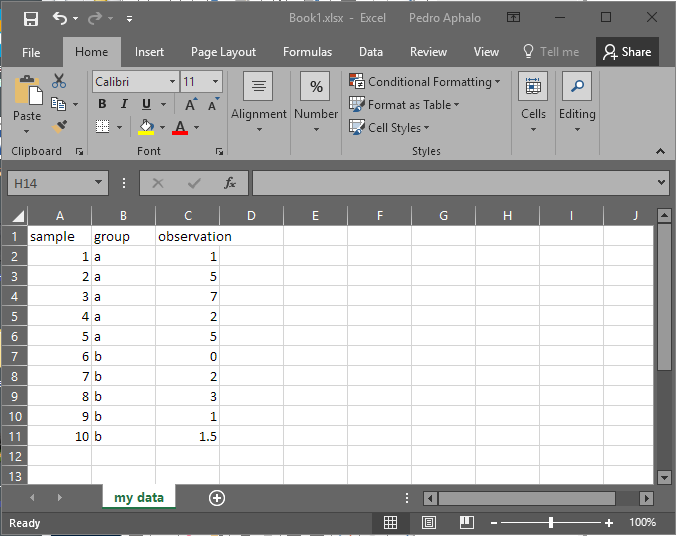
\includegraphics[width=0.75\textwidth]{figures/Book1-xlsx.png}
\end{center}

We first list the sheets contained in the workbook file with \Rfunction{excel\_sheets()}.
\begin{knitrout}\footnotesize
\definecolor{shadecolor}{rgb}{0.969, 0.969, 0.969}\color{fgcolor}\begin{kframe}
\begin{alltt}
\hlstd{sheets} \hlkwb{<-} \hlkwd{excel_sheets}\hlstd{(}\hlstr{"extdata/Book1.xlsx"}\hlstd{)}
\hlstd{sheets}
\end{alltt}
\begin{verbatim}
## [1] "my data"
\end{verbatim}
\end{kframe}
\end{knitrout}

In this case the argument passed to \code{sheet} is redundant, as there is only a single worksheet in the file. It is possible to use either the name of the sheet or a positional index (in this case \code{1} would be equivalent to \code{"my data"}). We use function \Rfunction{read\_excel()} to import the worksheet.
\begin{knitrout}\footnotesize
\definecolor{shadecolor}{rgb}{0.969, 0.969, 0.969}\color{fgcolor}\begin{kframe}
\begin{alltt}
\hlstd{Book1.df} \hlkwb{<-} \hlkwd{read_excel}\hlstd{(}\hlstr{"extdata/Book1.xlsx"}\hlstd{,} \hlkwc{sheet} \hlstd{=} \hlstr{"my data"}\hlstd{)}
\hlstd{Book1.df}
\end{alltt}
\begin{verbatim}
## # A tibble: 10 x 3
##    sample group observation
##     <dbl> <chr>       <dbl>
##  1      1 a             1  
##  2      2 a             5  
##  3      3 a             7  
##  4      4 a             2  
##  5      5 a             5  
##  6      6 b             0  
##  7      7 b             2  
##  8      8 b             3  
##  9      9 b             1  
## 10     10 b             1.5
\end{verbatim}
\end{kframe}
\end{knitrout}

Of the remaining arguments, \code{skip} is useful when we need to skip the top row of a worksheet.

\subsubsection['xlsx']{\pkgname{xlsx}}

\begin{knitrout}\footnotesize
\definecolor{shadecolor}{rgb}{0.969, 0.969, 0.969}\color{fgcolor}\begin{kframe}
\begin{alltt}
\hlkwd{citation}\hlstd{(}\hlkwc{package} \hlstd{=} \hlstr{"xlsx"}\hlstd{)}
\end{alltt}
\begin{verbatim}
## 
## To cite package 'xlsx' in publications use:
## 
##   Adrian A. Dragulescu and Cole Arendt (2018). xlsx: Read, Write,
##   Format Excel 2007 and Excel 97/2000/XP/2003 Files. R package
##   version 0.6.1. https://CRAN.R-project.org/package=xlsx
## 
## A BibTeX entry for LaTeX users is
## 
##   @Manual{,
##     title = {xlsx: Read, Write, Format Excel 2007 and Excel 97/2000/XP/2003 Files},
##     author = {Adrian A. Dragulescu and Cole Arendt},
##     year = {2018},
##     note = {R package version 0.6.1},
##     url = {https://CRAN.R-project.org/package=xlsx},
##   }
## 
## ATTENTION: This citation information has been auto-generated from
## the package DESCRIPTION file and may need manual editing, see
## 'help("citation")'.
\end{verbatim}
\end{kframe}
\end{knitrout}

Package \pkgname{xlsx} can be more difficult to install as it uses Java functions to do the actual work. However, it is more comprehensive, with functions both for reading and writing Excel worksheet and workbooks, in different formats. It also allows selecting regions of a worksheet to be imported.

Here we use function \Rfunction{read.xlsx()}, idexing the worksheet by name.

\begin{knitrout}\footnotesize
\definecolor{shadecolor}{rgb}{0.969, 0.969, 0.969}\color{fgcolor}\begin{kframe}
\begin{alltt}
\hlstd{Book1_xlsx.df} \hlkwb{<-} \hlkwd{read.xlsx}\hlstd{(}\hlstr{"extdata/Book1.xlsx"}\hlstd{,} \hlkwc{sheetName} \hlstd{=} \hlstr{"my data"}\hlstd{)}
\hlstd{Book1_xlsx.df}
\end{alltt}
\begin{verbatim}
##    sample group observation
## 1       1     a         1.0
## 2       2     a         5.0
## 3       3     a         7.0
## 4       4     a         2.0
## 5       5     a         5.0
## 6       6     b         0.0
## 7       7     b         2.0
## 8       8     b         3.0
## 9       9     b         1.0
## 10     10     b         1.5
\end{verbatim}
\end{kframe}
\end{knitrout}

As above, but indexing by a numeric index.

\begin{knitrout}\footnotesize
\definecolor{shadecolor}{rgb}{0.969, 0.969, 0.969}\color{fgcolor}\begin{kframe}
\begin{alltt}
\hlstd{Book1_xlsx2.df} \hlkwb{<-} \hlkwd{read.xlsx2}\hlstd{(}\hlstr{"extdata/Book1.xlsx"}\hlstd{,} \hlkwc{sheetIndex} \hlstd{=} \hlnum{1}\hlstd{)}
\hlstd{Book1_xlsx2.df}
\end{alltt}
\begin{verbatim}
##    sample group observation
## 1       1     a           1
## 2       2     a           5
## 3       3     a           7
## 4       4     a           2
## 5       5     a           5
## 6       6     b           0
## 7       7     b           2
## 8       8     b           3
## 9       9     b           1
## 10     10     b         1.5
\end{verbatim}
\end{kframe}
\end{knitrout}

With the three different functions we get a data frame or a tibble, which is compatible with data frames.
\begin{knitrout}\footnotesize
\definecolor{shadecolor}{rgb}{0.969, 0.969, 0.969}\color{fgcolor}\begin{kframe}
\begin{alltt}
\hlkwd{class}\hlstd{(Book1.df)}
\end{alltt}
\begin{verbatim}
## [1] "tbl_df"     "tbl"        "data.frame"
\end{verbatim}
\begin{alltt}
\hlkwd{class}\hlstd{(Book1_xlsx.df)}
\end{alltt}
\begin{verbatim}
## [1] "data.frame"
\end{verbatim}
\begin{alltt}
\hlkwd{class}\hlstd{(Book1_xlsx2.df)}
\end{alltt}
\begin{verbatim}
## [1] "data.frame"
\end{verbatim}
\end{kframe}
\end{knitrout}

However, the columns are imported differently. Both \code{Book1.df} and \code{Book1\_xlsx.df} differ only in that the second column, a character variable, has been converted into a factor or not. This is to be expected as packages in the \pkgname{tidyverse} suite default to preserving character variables as such, while base \Rlang functions convert them to factors. The third function, \Rfunction{read.xlsx2()}, did not decode numeric values correctly, and converted everything into factors. This function is reported as being much faster than \Rfunction{read.xlsx()}.
\begin{knitrout}\footnotesize
\definecolor{shadecolor}{rgb}{0.969, 0.969, 0.969}\color{fgcolor}\begin{kframe}
\begin{alltt}
\hlkwd{sapply}\hlstd{(Book1.df, class)}
\end{alltt}
\begin{verbatim}
##      sample       group observation 
##   "numeric" "character"   "numeric"
\end{verbatim}
\begin{alltt}
\hlkwd{sapply}\hlstd{(Book1_xlsx.df, class)}
\end{alltt}
\begin{verbatim}
##      sample       group observation 
##   "numeric"    "factor"   "numeric"
\end{verbatim}
\begin{alltt}
\hlkwd{sapply}\hlstd{(Book1_xlsx2.df, class)}
\end{alltt}
\begin{verbatim}
##      sample       group observation 
##    "factor"    "factor"    "factor"
\end{verbatim}
\end{kframe}
\end{knitrout}

With function \Rfunction{write.xlsx()} we can also write data frames out to Excel worksheets and even append new worksheets to an existing workbook.
\begin{knitrout}\footnotesize
\definecolor{shadecolor}{rgb}{0.969, 0.969, 0.969}\color{fgcolor}\begin{kframe}
\begin{alltt}
\hlkwd{set.seed}\hlstd{(}\hlnum{456321}\hlstd{)}
\hlstd{my.data} \hlkwb{<-} \hlkwd{data.frame}\hlstd{(}\hlkwc{x} \hlstd{=} \hlnum{1}\hlopt{:}\hlnum{10}\hlstd{,} \hlkwc{y} \hlstd{=} \hlnum{1}\hlopt{:}\hlnum{10} \hlopt{+} \hlkwd{rnorm}\hlstd{(}\hlnum{10}\hlstd{))}
\hlkwd{write.xlsx}\hlstd{(my.data,} \hlkwc{file} \hlstd{=} \hlstr{"extdata/my-data.xlsx"}\hlstd{,} \hlkwc{sheetName} \hlstd{=} \hlstr{"first copy"}\hlstd{)}
\hlkwd{write.xlsx}\hlstd{(my.data,} \hlkwc{file} \hlstd{=} \hlstr{"extdata/my-data.xlsx"}\hlstd{,} \hlkwc{sheetName} \hlstd{=} \hlstr{"second copy"}\hlstd{,} \hlkwc{append} \hlstd{=} \hlnum{TRUE}\hlstd{)}
\end{alltt}
\end{kframe}
\end{knitrout}

When opened in Excel we get a workbook, containing two worksheets, named using the arguments we passed through \code{sheetName} in the code chunk above.
\begin{center}
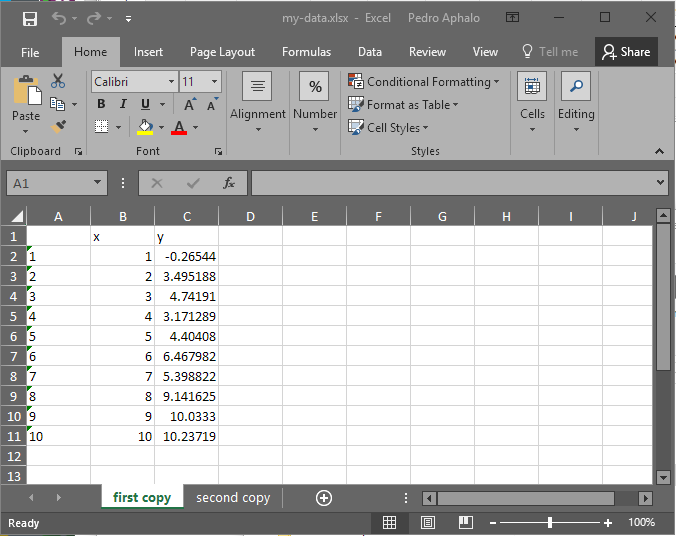
\includegraphics[width=0.75\textwidth]{figures/my-data-xlsx.png}
\end{center}

\begin{playground}
If you have some worksheet files available, import them into R, to get a feel of how the way data is organized in the worksheets affects how easy or difficult it is to read the data from them.
\end{playground}

\subsubsection['xml2']{\pkgname{xml2}}

\begin{knitrout}\footnotesize
\definecolor{shadecolor}{rgb}{0.969, 0.969, 0.969}\color{fgcolor}\begin{kframe}
\begin{alltt}
\hlkwd{citation}\hlstd{(}\hlkwc{package} \hlstd{=} \hlstr{"xml2"}\hlstd{)}
\end{alltt}
\begin{verbatim}
## 
## To cite package 'xml2' in publications use:
## 
##   Hadley Wickham, James Hester and Jeroen Ooms (2018). xml2: Parse
##   XML. R package version 1.2.0.
##   https://CRAN.R-project.org/package=xml2
## 
## A BibTeX entry for LaTeX users is
## 
##   @Manual{,
##     title = {xml2: Parse XML},
##     author = {Hadley Wickham and James Hester and Jeroen Ooms},
##     year = {2018},
##     note = {R package version 1.2.0},
##     url = {https://CRAN.R-project.org/package=xml2},
##   }
\end{verbatim}
\end{kframe}
\end{knitrout}

Several modern data exchange formats are based on the XML standard format which uses schema for flexibility. Package \pkgname{xml2} provides functions for reading and parsing such files, as well as HTML files. This is a vast subject, of which I will only give a brief introduction.

We first read a very simple web page with function \Rfunction{read\_html()}.

\begin{knitrout}\footnotesize
\definecolor{shadecolor}{rgb}{0.969, 0.969, 0.969}\color{fgcolor}\begin{kframe}
\begin{alltt}
\hlstd{web_page} \hlkwb{<-} \hlkwd{read_html}\hlstd{(}\hlstr{"http://r4photobiology.info/R/index.html"}\hlstd{)}
\hlkwd{html_structure}\hlstd{(web_page)}
\end{alltt}
\begin{verbatim}
## <html>
##   <head>
##     <title>
##       {text}
##     <meta [name, content]>
##     <meta [name, content]>
##     <meta [name, content]>
##   <body>
##     {text}
##     <hr>
##     <h1>
##       {text}
##     {text}
##     <hr>
##     <p>
##       {text}
##       <a [href]>
##         {text}
##       {text}
##     {text}
##     <address>
##       {text}
##     {text}
\end{verbatim}
\end{kframe}
\end{knitrout}

And we extract the text from its \code{title} attribute, using functions \Rfunction{xml\_find\_all()} and \Rfunction{xml\_text()}.

\begin{knitrout}\footnotesize
\definecolor{shadecolor}{rgb}{0.969, 0.969, 0.969}\color{fgcolor}\begin{kframe}
\begin{alltt}
\hlkwd{xml_text}\hlstd{(}\hlkwd{xml_find_all}\hlstd{(web_page,} \hlstr{".//title"}\hlstd{))}
\end{alltt}
\begin{verbatim}
## [1] "r4photobiology repository"
\end{verbatim}
\end{kframe}
\end{knitrout}

The functions defined in this package and in package \pkgname{XML} can be used to ``harvest'' data from web pages, but also to read data from files using formats that are defined through XML schemas.

\subsection{Statistical software}\label{sec:files:stat}

There are two different comprehensive packages for importing data saved from other statistical such as SAS, Statistica, SPSS, etc. The long time ``standard'' the \pkgname{foreign} package and the much newer \pkgname{haven}. In the case of files saved with old versions of statistical programs, functions from \pkgname{foreign} tend to be more more robust than those from \pkgname{haven}.

\subsubsection[foreign]{\pkgname{foreign}}

\begin{knitrout}\footnotesize
\definecolor{shadecolor}{rgb}{0.969, 0.969, 0.969}\color{fgcolor}\begin{kframe}
\begin{alltt}
\hlkwd{citation}\hlstd{(}\hlkwc{package} \hlstd{=} \hlstr{"foreign"}\hlstd{)}
\end{alltt}
\begin{verbatim}
## 
## To cite package 'foreign' in publications use:
## 
##   R Core Team (2018). foreign: Read Data Stored by 'Minitab', 'S',
##   'SAS', 'SPSS', 'Stata', 'Systat', 'Weka', 'dBase', .... R
##   package version 0.8-71.
##   https://CRAN.R-project.org/package=foreign
## 
## A BibTeX entry for LaTeX users is
## 
##   @Manual{,
##     title = {foreign: Read Data Stored by 'Minitab', 'S', 'SAS', 'SPSS', 'Stata',
## 'Systat', 'Weka', 'dBase', ...},
##     author = {{R Core Team}},
##     year = {2018},
##     note = {R package version 0.8-71},
##     url = {https://CRAN.R-project.org/package=foreign},
##   }
\end{verbatim}
\end{kframe}
\end{knitrout}

Functions in this package allow to import data from files saved by several foreign statistical analysis programs, including \pgrmname{SAS}, \pgrmname{Stata} and \pgrmname{SPPS} among others, and a function for writing data into files with formats native to these three programs. Documentation is included with \Rlang describing them in \emph{R Data Import/Export}. As a simple example we use function \Rfunction{read.spss()} to read a \texttt{.sav} file, saved with a recent version of \pgrmname{SPSS}.

\begin{knitrout}\footnotesize
\definecolor{shadecolor}{rgb}{0.969, 0.969, 0.969}\color{fgcolor}\begin{kframe}
\begin{alltt}
\hlstd{my_spss.df} \hlkwb{<-} \hlkwd{read.spss}\hlstd{(}\hlkwc{file} \hlstd{=} \hlstr{"extdata/my-data.sav"}\hlstd{,} \hlkwc{to.data.frame} \hlstd{=} \hlnum{TRUE}\hlstd{)}
\end{alltt}


{\ttfamily\noindent\itshape\color{messagecolor}{\#\# re-encoding from UTF-8}}\begin{alltt}
\hlkwd{head}\hlstd{(my_spss.df)}
\end{alltt}
\begin{verbatim}
##   block       treat mycotreat water1 pot harvest meas_order spad psi H_mm
## 1     0 Watered, EM         1      1  14       1         NA   NA  NA   67
## 2     0 Watered, EM         1      1  52       1         NA   NA  NA   44
## 3     0 Watered, EM         1      1 111       1         NA   NA  NA   65
## 4     0 Watered, EM         1      1 127       1         NA   NA  NA   78
## 5     0 Watered, EM         1      1 230       1         NA   NA  NA   71
## 6     0 Watered, EM         1      1 258       1         NA   NA  NA  100
##    d_mm pot_plant_g plant_g tag_g pot_g leaf_area harvest_date stem_g
## 1 2.115          NA      NA    NA    NA    35.883  13653705600 0.0372
## 2 1.285          NA      NA    NA    NA    16.938  13653705600 0.0139
## 3 1.685          NA      NA    NA    NA    38.056  13653705600 0.0279
## 4 1.870          NA      NA    NA    NA    38.469  13653705600 0.0389
## 5 1.900          NA      NA    NA    NA    39.917  13653705600 0.0446
## 6 1.810          NA      NA    NA    NA    45.968  13653705600 0.0513
##   leaves_g green_leaves save_order waterprcnt height_1 height_2 height_3
## 1   0.1685       0.0542          1         NA       23       34       55
## 2   0.0626       0.0443          2         NA       10       21       37
## 3   0.1522       0.0511          3         NA       12       27       48
## 4   0.1462       0.0500          4         NA       30       40       64
## 5   0.1696       0.0677          5         NA       28       37       60
## 6   0.1959       0.0741          6         NA       42       60       84
##   height_4 diam_1 height_5 diam_2
## 1       NA     NA       NA     NA
## 2       NA     NA       NA     NA
## 3       NA     NA       NA     NA
## 4       NA     NA       NA     NA
## 5       NA     NA       NA     NA
## 6       NA     NA       NA     NA
\end{verbatim}
\end{kframe}
\end{knitrout}

Dates were not converted into \Rlang datetime objects, but instead into numbers.

A second example, this time with a simple \code{.sav} file saved 15 years ago.

\begin{knitrout}\footnotesize
\definecolor{shadecolor}{rgb}{0.969, 0.969, 0.969}\color{fgcolor}\begin{kframe}
\begin{alltt}
\hlstd{thiamin.df} \hlkwb{<-} \hlkwd{read.spss}\hlstd{(}\hlkwc{file} \hlstd{=} \hlstr{"extdata/thiamin.sav"}\hlstd{,} \hlkwc{to.data.frame} \hlstd{=} \hlnum{TRUE}\hlstd{)}
\hlkwd{head}\hlstd{(thiamin.df)}
\end{alltt}
\begin{verbatim}
##   THIAMIN CEREAL
## 1     5.2  wheat
## 2     4.5  wheat
## 3     6.0  wheat
## 4     6.1  wheat
## 5     6.7  wheat
## 6     5.8  wheat
\end{verbatim}
\end{kframe}
\end{knitrout}

Another example, for a Systat file saved on an PC more than 20 years ago, and rea.

\begin{knitrout}\footnotesize
\definecolor{shadecolor}{rgb}{0.969, 0.969, 0.969}\color{fgcolor}\begin{kframe}
\begin{alltt}
\hlstd{my_systat.df} \hlkwb{<-} \hlkwd{read.systat}\hlstd{(}\hlkwc{file} \hlstd{=} \hlstr{"extdata/BIRCH1.SYS"}\hlstd{)}
\hlstd{my_systat.df}
\end{alltt}
\begin{verbatim}
##     CONT DENS BLOCK SEEDL VITAL BASE ANGLE HEIGHT DIAM
## 1      1    1     1     2    44    2     0      1   53
## 2      1    1     1     2    41    2     1      2   70
## 3      1    1     1     2    21    2     0      1   65
## 4      1    1     1     2    15    3     0      1   79
## 5      1    1     1     2    37    3     0      1   71
## 6      1    1     1     2    29    2     1      1   43
## 7      1    1     1     1    30    0    NA     NA   NA
## 8      1    1     1     1    28    0    NA     NA   NA
## 9      1    1     1     1    37    3     2      1   74
## 10     1    1     1     1    26    3     1      3   71
## 11     1    1     1     1    27    3     0      1   64
## 12     1    1     1     1    45    0    NA     NA   NA
## 13     1    1     4     2    41    3     2      1   76
## 14     1    1     4     2    32    1     1      3   35
## 15     1    1     4     2    19    3     1      2   79
## 16     1    1     4     2    20    2     0      2   70
## 17     1    1     4     2     3    2     2      3   75
## 18     1    1     4     2     5    0    NA     NA   NA
## 19     1    1     4     1    28    2     1      2   80
## 20     1    1     4     1    41    2     1      3   73
## 21     1    1     4     1    36    1     0      1   21
## 22     1    1     4     1    43    2     0      2   51
## 23     1    1     4     1    22    2     1      2   66
## 24     1    1     4     1    31    3     1      2   84
## 25     1    1     3     2    30    2     0      1   49
## 26     1    1     3     2     4    2     2      1   42
## 27     1    1     3     2    35    3     2      2   90
## 28     1    1     3     2    43    2     1      2   60
## 29     1    1     3     2    12    3     0      1   65
## 30     1    1     3     1    35    2     0      1   61
## 31     1    1     3     1    36    2     0      2   65
## 32     1    1     3     1     7    3     2      1   83
## 33     1    1     3     1     9    2     3      2   68
## 34     1    1     3     1    20    2     1      1   65
## 35     1    1     3     1    11    2     1      1   53
## 36     1    1     3     1    14    2     0      1   60
## 37     1    1     1     3    30    2     0      1   59
## 38     1    1     1     3    15    2     2      2   65
## 39     1    1     1     3    14    2     2      2   77
## 40     1    1     1     3    32    3     0      1   72
## 41     1    1     1     3    38    3     2      2   78
## 42     1    1     1     3    13    2     1      1   56
## 43     1    1     4     2    41    3     2      1   77
## 44     1    1     4     2    32    1     1      2   34
## 45     1    1     4     2    19    3     1      2   80
## 46     1    1     4     2    20    3     0      2   70
## 47     1    1     4     2     3    2     1      2   75
## 48     1    1     4     1    28    3     1      2   80
## 49     1    1     4     1    41    2     1      2   73
## 50     1    1     4     1    36    1     0      1   21
## 51     1    1     4     1    43    2     0      1   51
## 52     1    1     4     1    22    2     1      2   66
## 53     1    1     4     1    31    3     1      2   84
## 54     1    1     3     2    30    2     0      1   49
## 55     1    1     3     2     4    2     2      1   42
## 56     1    1     3     2    35    3     2      2   89
## 57     1    1     3     2    43    2     1      2   60
## 58     1    1     3     2    12    3     0      1   65
## 59     1    1     3     1    35    2     0      1   60
## 60     1    1     3     1    36    2     0      1   66
## 61     1    1     3     1     7    3     2      1   83
## 62     1    1     3     1     9    2     3      2   68
## 63     1    1     3     1    20    2     1      1   65
## 64     1    1     3     1    11    2     1      1   54
## 65     1    1     3     1    14    2     0      1   60
## 66     1    1     2     3    29    2     1      1   47
## 67     1    1     2     3    27    2     0      1   67
## 68     1    1     2     3    45    3     1      1   74
## 69     1    1     2     3    40    0    NA     NA   NA
## 70     1    1     2     3    33    1     1      1   47
## 71     1    1     2     3    19    2     1      1   57
## 72     1    1     2     2    18    3     0      1   74
## 73     1    1     2     1     2    2     0      3   71
## 74     1    1     2     2    33    3     1      1   80
## 75     1    1     2     1    16    0    NA     NA   NA
## 76     1    1     2     1    44    0    NA     NA   NA
## 77     1    1     2     1    34    2     1      1   54
## 78     1    1     2     2    32    3     0      1   77
## 79     1    1     2     2    21    3     1      1   74
## 80     1    1     2     1    13    3     1      1   69
## 81     1    1     2     1     3    3     1      1   72
## 82     1    1     2     2     7    0    NA     NA   NA
## 83     1    1     2     2    39    2     1      1   54
## 84     1    2     1     4     5    2     1      2   67
## 85     1    2     1     4    14    2     1      2   46
## 86     1    2     1     4    17    2     1      1   64
## 87     1    2     1     3     7    3     0      1  100
## 88     1    2     1     3     9    3     2      2   69
## 89     1    2     1     3    13    3     1      1   74
## 90     1    2     1     3    12    3     0      1   71
## 91     1    2     3     1     1    0    NA     NA   NA
## 92     1    2     3     1     6    2     2      1   35
## 93     1    2     3     1    15    2     0      1   38
## 94     1    2     3     4    10    2     1      1   65
## 95     1    2     3     4     1    2     0      2   72
## 96     1    2     3     3    23    2     2      2   66
## 97     1    2     3     3    20    1     0      1   17
## 98     1    2     3     3    12    3     2      1   71
## 99     1    2     3     3    21    2     1      1   43
## 100    1    2     3     2     4    2     0      1   44
## 101    1    2     3     2    14    1     0      1   20
## 102    1    2     3     2    18    2     1      2   57
## 103    1    2     3     5    18    2     0      2   54
## 104    1    2     3     5     9    2     3      2   55
## 105    1    2     3     5    16    2     1      1   57
## 106    1    2     3     5    17    3     0      1   73
## 107    1    2     3     4    16    2     1      1   30
## 108    1    2     4     1    14    3     1      1   84
## 109    1    2     4     1    12    3     0      1   75
## 110    1    2     4     3    17    2     0      1   65
## 111    1    2     4     3    15    3     0      1   81
## 112    1    2     4     2     5    2     1      1   62
## 113    1    2     4     2     7    3     0      1   84
## 114    1    2     4     2     6    2     0      1   66
## 115    1    2     4     1    17    3     1      1   73
## 116    1    2     4     1    10    3     0      1   88
## 117    1    2     4     3     5    2     0      1   61
## 118    1    2     2     3    18    3     0      1   87
## 119    1    2     2     3    21    3     0      1   74
## 120    1    2     2     1     3    2     2      3   60
## 121    1    2     2     1    13    2     0      2   63
## 122    1    2     2     1    12    3     1      2   69
## 123    1    2     2     3     2    3     0      1   81
## 124    1    2     4     3     5    2     0      1   61
## 125    1    2     2     3    18    3     0      1   87
## 126    1    2     2     3    21    3     0      1   74
## 127    1    2     2     1     3    2     2      2   60
## 128    1    2     2     1    13    2     0      2   63
## 129    1    2     2     1    12    3     1      1   70
## 130    1    2     2     3     2    3     0      1   81
## 131    1    2     1     1     5    3     1      1   72
## 132    1    2     1     1    21    2     0      1   48
## 133    1    2     1     1    12    2     0      1   44
## 134    1    2     1     1    10    2     1      2   50
## 135    1    2     4     4    22    3     0      1   80
## 136    1    2     4     4     5    2     1      1   53
## 137    1    2     4     4     2    3     0      1   79
## 138    1    2     4     5    22    3     1      2   77
## 139    1    2     4     5    20    2     1      1   52
## 140    1    2     4     5    16    3     1      1   77
## 141    1    2     2     2     4    3     0      1   75
## 142    1    2     2     2     7    3     1      1   83
## 143    1    2     2     2    13    2     1      1   48
## 144    1    2     2     4    21    2     1      1   55
## 145    1    2     2     4    20    2     1      1   55
## 146    1    2     2     4    16    3     0      1   81
## 147    1    2     2     4    11    3     1      2   76
## 148    1    2     1     2     4    2     2      1   64
## 149    1    2     1     2     6    3     1      1   87
## 150    1    2     1     2     5    2     2      1   60
## 151    1    3     3     1     4    2     0      2   63
## 152    1    3     3     2     4    2     0      1   70
## 153    1    3     3     2     5    3     1      1   82
## 154    1    3     3     3     4    0     0      1   95
## 155    1    3     3     6     3    2     0      1   51
## 156    1    3     3     6     6    2     0      2   49
## 157    1    3     3     7    10    2     0      2   66
## 158    1    3     3     8     7    3     1      2   74
## 159    1    3     3     1     2    2     0      1   54
## 160    1    3     3     6     6    2     0      1   49
## 161    1    3     3     6     3    2     0      1   51
## 162    1    3     3     7    10    2     1      1   66
## 163    1    3     3     8     7    3     0      2   74
## 164    1    3     3     1     2    2     0      1   54
## 165    1    3     1     8     2    2     0      2   68
## 166    1    3     4     3    10    3     1      2   80
## 167    1    3     4     2    10    3     1      1   87
## 168    1    3     4     9     8    1     0      1   36
## 169    1    3     4     9     3    1     3      2   56
## 170    1    3     3     5    12    3     1      2   82
## 171    1    3     1     8     8    2     0      1   70
## 172    1    3     4     1    11    2     0      1   51
## 173    1    3     4     6     2    2     1      1   52
## 174    1    3     4     8     9    2     0      1   67
## 175    1    3     3     5    10    2     0      1   42
## 176    1    3     1     7    10    3     1      1   78
## 177    1    3     4     1     8    2     0      1   61
## 178    1    3     4     6    10    2     1      1   44
## 179    1    3     4     8     5    3     1      1   91
## 180    1    3     3     4     6    3     1      1   91
## 181    1    3     4     7     1    3     0      1   80
## 182    1    3     4     5     2    2     0      1   51
## 183    1    3     4     4    12    2     0      1   55
## 184    1    3     1     7     6    2     1      1   68
## 185    1    3     4     4     4    2     0      1   68
## 186    1    3     4     5    10    3     0      1   78
## 187    1    3     4     7     8    2     0      1   27
## 188    1    3     3    10    13    2     1      2   75
## 189    1    3     3    10    10    2     1      2   61
## 190    1    3     3     9     8    2     0      1   60
## 191    1    3     3     9     2    3     0      1   85
## 192    1    3     1     5     3    3     1      1   81
## 193    1    3     2     5     1    3     1      2   77
## 194    1    3     1     1     3    3     1      1   86
## 195    1    3     1     2     3    3     0      2   75
## 196    1    3     1     5     6    2     0      1   63
## 197    1    3     2     5     9    3     1      1   74
## 198    1    3     1     1     2    2     1      1   62
## 199    1    3     1     2    12    2     0      1   46
## 200    1    3     1     6    12    2     0      1   46
## 201    1    3     1     3     8    2     3      1   63
## 202    1    3     2     6     2    3     2      1   75
## 203    1    3     2     8     9    2     1      1   39
## 204    1    3     2     1     5    2     1      2   58
## 205    1    3     2     3    12    2     1      1   61
## 206    1    3     1     4     9    2     1      1   52
## 207    1    3     2     4    11    2     1      1   54
## 208    1    3     2     1     9    3     1      1   76
## 209    1    3     2     8    12    2     0      1   44
## 210    1    3     2     6    13    3     1      1   71
## 211    1    3     2     2     3    2     1      2   49
## 212    1    3     2     2    10    3     0      1   67
## 213    1    3     2     7     6    2     1      1   63
## 214    1    3     2     7     2    3     0      1   75
## 215    1    3     1     4     3    2     1      1   57
## 216    2    1     1     4    12    2     1      3   64
## 217    2    1     1     4    13    0    NA     NA   NA
## 218    2    1     1     1    17    3     1      1   92
## 219    2    1     1     3    16    3     2      1  106
## 220    2    1     1     3     5    3     1      1   93
## 221    2    1     1     3    13    3     0      1  101
## 222    2    1     1     1    19    3     0      1   72
## 223    2    1     1     4     1    3     0      2   90
## 224    2    1     1     2     7    3     0      2   93
## 225    2    1     1     2    19    3     0      1   90
## 226    2    1     1     2    20    3     0      1   87
## 227    2    1     1     2    11    3     0      2   96
## 228    2    1     1     1    15    3     1      2   90
## 229    2    1     1     3    15    3     1      1   96
## 230    2    1     1     1    27    2     2      2   46
## 231    2    1     2     3    18    2     0      1   71
## 232    2    1     3     2     6    3     0      1  101
## 233    2    1     2     3     9    3     0      2   76
## 234    2    1     3     2    28    3     1      1   82
## 235    2    1     3     4    19    3     0      1   75
## 236    2    1     2     3    26    2     1      1   60
## 237    2    1     3     2    15    3     1      1   89
## 238    2    1     3     1     3    3     1      1   92
## 239    2    1     3     4    25    2     0      2   67
## 240    2    1     2     3    27    3     0      1   87
## 241    2    1     3     2    25    2     1      1   66
## 242    2    1     3     1    22    2     2      1   61
## 243    2    1     3     4    11    3     1      1  100
## 244    2    1     3     1    10    3     0      1   86
## 245    2    1     3     1    15    2     0      1   61
## 246    2    1     3     4    17    3     0      1   92
## 247    2    1     4     1    17    3     1      1   94
## 248    2    1     4     1    22    2     1      1   70
## 249    2    1     3     3    22    3     1      1   85
## 250    2    1     3     3    21    3     0      2   85
## 251    2    1     3     3     4    0    NA     NA   NA
## 252    2    1     3     3    12    0    NA     NA   NA
## 253    2    1     4     1     3    3     1      1   80
## 254    2    1     4     1    21    3     0      1   74
## 255    2    1     4     2     3    3     1      1   59
## 256    2    1     4     2    19    3     1      2   82
## 257    2    1     4     2    24    2     0      2   82
## 258    2    1     4     2    11    2     1      2   70
## 259    2    1     4     3    28    1     3      1   28
## 260    2    1     4     3     7    2     1      1   69
## 261    2    1     4     3    11    2     1      3   82
## 262    2    1     4     3    13    3     0      1   89
## 263    2    1     2     2    24    2     0      1   76
## 264    2    1     2     2     3    3     1      1   78
## 265    2    1     2     2    12    3     1      1   88
## 266    2    1     2     1     4    3     1      2   80
## 267    2    1     2     1    27    3     1      1   86
## 268    2    1     2     1    26    3     0      1   81
## 269    2    1     2     1    11    3     1      1   88
## 270    2    1     2     2     8    2     1      1   34
## 271    2    1     2     4    12    3     1      1   83
## 272    2    1     2     4     5    3     1      1   86
## 273    2    1     2     4    15    3     1      1   88
## 274    2    1     2     4    24    2     1      1   54
## 275    2    2     2     8     6    2     0      1   70
## 276    2    2     4     1    12    3     0      1   78
## 277    2    2     3     5     1    3     1      1   99
## 278    2    2     3     2    10    3     1      1   90
## 279    2    2     3     1     4    0    NA     NA   NA
## 280    2    2     3     5    10    3     1      1   80
## 281    2    2     2     8    12    3     0      1   91
## 282    2    2     3     3    13    0    NA     NA   NA
## 283    2    2     3     4     2    3     0      1   88
## 284    2    2     4     7     8    3     0      2   86
## 285    2    2     4     7     5    3     2      1   79
## 286    2    2     3     4     3    3     0      2   83
## 287    2    2     3     6     6    3     1      1   99
## 288    2    2     4     1    10    2     0      2   68
## 289    2    2     3     6    13    3     0      1   86
## 290    2    2     1     3     1    2     1      2   82
## 291    2    2     1     6    12    3     1      1   73
## 292    2    2     1     7     6    3     2      2   82
## 293    2    2     1     7     3    3     0      2   86
## 294    2    2     1     1     7    3     0      1   92
## 295    2    2     1     4     9    3     0      1   78
## 296    2    2     1     5     4    2     2      1   67
## 297    2    2     1     8     1    3     0      1   87
## 298    2    2     3     1     8    1     2      2   52
## 299    2    2     1     1    14    3     0      2   90
## 300    2    2     1     4    12    3     0      1   86
## 301    2    2     1     5     9    3     1      3   97
## 302    2    2     1     8     9    3     0      1   85
## 303    2    2     3     1     6    3     0      1  116
## 304    2    2     1     2     6    2     2      3   70
## 305    2    2     1     2    10    1     2      1   39
## 306    2    2     1     3     6    3     2      1   91
## 307    2    2     1     6     2    3     1      2   83
## 308    2    2     4     2    10    2     1      3   62
## 309    2    2     4     2     2    2     1      2   72
## 310    2    2     2     3     3    2     0      4   59
## 311    2    2     4     6     7    3     1      1   76
## 312    2    2     2     3    10    3     0      1   82
## 313    2    2     4     6    12    3     0      1   69
## 314    2    2     4     8    13    3     1      1   92
## 315    2    2     2     4    14    3     1      1   85
## 316    2    2     2     7    11    3     1      2   95
## 317    2    2     4     3     6    3     0      1   86
## 318    2    2     2     7    14    3     0      3   97
## 319    2    2     4     5    12    3     1      1  106
## 320    2    2     4     8     6    3     1      1  103
## 321    2    2     2     4     9    3     0      2   97
## 322    2    2     4     3     3    3     1      1   95
## 323    2    2     4     5     2    3     0      1   80
## 324    2    2     4     4    11    3     1      1   85
## 325    2    2     4     4     9    3     1      1   86
## 326    2    2     2     2     6    3     0      1   97
## 327    2    2     2     2     7    2     0      1   69
## 328    2    2     2     1     4    2     0      1   76
## 329    2    2     2     1     6    3     0      1   79
## 330    2    2     2     5     3    3     1      1   94
## 331    2    2     2     5    10    3     1      2   91
## 332    2    2     2     6    10    3     0      1   83
## 333    2    2     2     6     4    3     0      1   94
## 334    2    3     3     1     6    3     0      2   96
## 335    2    3     3     6     7    3     0      1   73
## 336    2    3     2     4     5    3     0      1   78
## 337    2    3     3     7     2    3     0      1   86
## 338    2    3     2     9     3    2     0      1   52
## 339    2    3     3    11     4    3     0      1   92
## 340    2    3     3     8     3    3     0      1   81
## 341    2    3     3    13     7    3     1      1  102
## 342    2    3     3    12     6    3     0      1  113
## 343    2    3     3     3     3    3     0      1  114
## 344    2    3     1     3     3    2     1      1   51
## 345    2    3     1    12     6    3     1      1  106
## 346    2    3     1     2     8    3     0      1   99
## 347    2    3     1     8     6    3     0      1   95
## 348    2    3     1     1     5    0    NA     NA   NA
## 349    2    3     1     7     3    3     0      1   71
## 350    2    3     1     4     4    3     1      1   81
## 351    2    3     1    11     2    3     0      1   75
## 352    2    3     3     2     4    3     1      1   67
## 353    2    3     3     2     3    0    NA     NA   NA
## 354    2    3     1    15     1    3     0      2   88
## 355    2    3     2     3     1    3     0      1   98
## 356    2    3     2     1     2    3     1      1   84
## 357    2    3     2     2     7    3     0      1   82
## 358    2    3     2     8     7    2     0      1   43
## 359    2    3     2     7     3    3     0      1   84
## 360    2    3     2     6     2    3     0      1   62
## 361    2    3     2    13     5    2     0      1   34
## 362    2    3     2    11     4    3     1      1   81
## 363    2    3     1    13     1    3     0      2   97
## 364    2    3     4     8     7    3     0      1   83
## 365    2    3     4     7     3    3     0      2   79
## 366    2    3     4     3     4    3     0      1   84
## 367    2    3     4     9     7    2     0      1   56
## 368    2    3     4     4     7    2     0      1   52
## 369    2    3     4     2     6    2     0      1   63
## 370    2    3     1    14     4    3     1      2  115
## 371    2    3     4     1     4    1     0      3   79
## 372    2    3     2    10     2    3     1      1   89
## 373    2    3     4    10     7    2     0      1   63
## 374    2    3     2    15     7    3     1      1   88
## 375    2    3     4    15     5    2     1      1   59
## 376    2    3     2     5     5    2     1      2   70
## 377    2    3     2    14     6    3     0      1   84
## 378    2    3     4     5     5    3     0      1   79
## 379    2    3     4     6     6    3     0      1   88
## 380    2    3     4    14     5    3     0      1   98
## 381    2    3     4    13     7    3     0      1   77
## 382    2    3     3     4     2    2     0      1   67
## 383    2    3     3     5     3    2     0      1   58
## 384    2    3     4    11     4    2     0      1   72
## 385    2    3     4    12     3    3     0      1  103
## 386    2    3     3    10     6    3     0      1   71
## 387    2    3     3     9     3    3     0      1  112
## 388    2    3     3    15     6    3     1      1   73
## 389    2    3     3    14     7    3     1      1   97
## 390    2    3     1     5     1    3     1      1   88
## 391    2    3     1     6     2    3     1      1   93
## 392    2    3     2    12     4    3     0      1   89
## 393    2    3     1    10     4    2     1      1   67
## 394    2    3     1     9     4    3     0      1   84
\end{verbatim}
\end{kframe}
\end{knitrout}

The functions in \pkgname{foreign} can return data frames, but not always this is the default.

\subsubsection[haven]{\pkgname{haven}}

\begin{knitrout}\footnotesize
\definecolor{shadecolor}{rgb}{0.969, 0.969, 0.969}\color{fgcolor}\begin{kframe}
\begin{alltt}
\hlkwd{citation}\hlstd{(}\hlkwc{package} \hlstd{=} \hlstr{"haven"}\hlstd{)}
\end{alltt}
\begin{verbatim}
## 
## To cite package 'haven' in publications use:
## 
##   Hadley Wickham and Evan Miller (2019). haven: Import and Export
##   'SPSS', 'Stata' and 'SAS' Files. R package version 2.1.1.
##   https://CRAN.R-project.org/package=haven
## 
## A BibTeX entry for LaTeX users is
## 
##   @Manual{,
##     title = {haven: Import and Export 'SPSS', 'Stata' and 'SAS' Files},
##     author = {Hadley Wickham and Evan Miller},
##     year = {2019},
##     note = {R package version 2.1.1},
##     url = {https://CRAN.R-project.org/package=haven},
##   }
\end{verbatim}
\end{kframe}
\end{knitrout}

The recently released package \pkgname{haven} is less ambitious in scope, providing read and write functions for only three file formats: \pgrmname{SAS}, \pgrmname{Stata} and \pgrmname{SPSS}. On the other hand \pkgname{haven} provides flexible ways to convert the different labelled values that cannot be directly mapped to normal \Rlang modes. They also decode dates and times according to the idiosyncrasies of each of these file formats. The returned \Rclass{tibble} objects in cases when the imported file contained labelled values needs some further work from the user before obtaining `normal' data-frame-compatible \Rclass{tibble} objects.

We here use function \Rfunction{read\_sav()} to import here a \code{.sav} file saved by a recent version of \pgrmname{SPSS}.

\begin{knitrout}\footnotesize
\definecolor{shadecolor}{rgb}{0.969, 0.969, 0.969}\color{fgcolor}\begin{kframe}
\begin{alltt}
\hlstd{my_spss.tb} \hlkwb{<-} \hlkwd{read_sav}\hlstd{(}\hlkwc{file} \hlstd{=} \hlstr{"extdata/my-data.sav"}\hlstd{)}
\hlstd{my_spss.tb}
\end{alltt}
\begin{verbatim}
## # A tibble: 372 x 29
##    block   treat mycotreat water1   pot harvest meas_order  spad   psi
##    <dbl> <dbl+l>     <dbl>  <dbl> <dbl>   <dbl>      <dbl> <dbl> <dbl>
##  1     0 1 [Wat~         1      1    14       1         NA    NA    NA
##  2     0 1 [Wat~         1      1    52       1         NA    NA    NA
##  3     0 1 [Wat~         1      1   111       1         NA    NA    NA
##  4     0 1 [Wat~         1      1   127       1         NA    NA    NA
##  5     0 1 [Wat~         1      1   230       1         NA    NA    NA
##  6     0 1 [Wat~         1      1   258       1         NA    NA    NA
##  7     0 1 [Wat~         1      1   363       1         NA    NA    NA
##  8     0 1 [Wat~         1      1   400       1         NA    NA    NA
##  9     0 1 [Wat~         1      1   424       1         NA    NA    NA
## 10     0 1 [Wat~         1      1   443       1         NA    NA    NA
## # ... with 362 more rows, and 20 more variables: H_mm <dbl>, d_mm <dbl>,
## #   pot_plant_g <dbl>, plant_g <dbl>, tag_g <dbl>, pot_g <dbl>,
## #   leaf_area <dbl>, harvest_date <date>, stem_g <dbl>, leaves_g <dbl>,
## #   green_leaves <dbl>, save_order <dbl>, waterprcnt <dbl>,
## #   height_1 <dbl>, height_2 <dbl>, height_3 <dbl>, height_4 <dbl>,
## #   diam_1 <dbl>, height_5 <dbl>, diam_2 <dbl>
\end{verbatim}
\begin{alltt}
\hlkwd{head}\hlstd{(my_spss.tb}\hlopt{$}\hlstd{harvest_date)}
\end{alltt}
\begin{verbatim}
## [1] "2015-06-15" "2015-06-15" "2015-06-15" "2015-06-15" "2015-06-15"
## [6] "2015-06-15"
\end{verbatim}
\end{kframe}
\end{knitrout}

In this case the dates are correctly decoded.

And an \pgrmname{SPSS}'s \code{.sav} file saved 15 years ago.

\begin{knitrout}\footnotesize
\definecolor{shadecolor}{rgb}{0.969, 0.969, 0.969}\color{fgcolor}\begin{kframe}
\begin{alltt}
\hlstd{thiamin.tb} \hlkwb{<-} \hlkwd{read_sav}\hlstd{(}\hlkwc{file} \hlstd{=} \hlstr{"extdata/thiamin.sav"}\hlstd{)}
\hlstd{thiamin.tb}
\end{alltt}
\begin{verbatim}
## # A tibble: 24 x 2
##    THIAMIN     CEREAL
##      <dbl>  <dbl+lbl>
##  1     5.2 1 [wheat] 
##  2     4.5 1 [wheat] 
##  3     6   1 [wheat] 
##  4     6.1 1 [wheat] 
##  5     6.7 1 [wheat] 
##  6     5.8 1 [wheat] 
##  7     6.5 2 [barley]
##  8     8   2 [barley]
##  9     6.1 2 [barley]
## 10     7.5 2 [barley]
## # ... with 14 more rows
\end{verbatim}
\begin{alltt}
\hlstd{thiamin.tb} \hlkwb{<-} \hlkwd{as_factor}\hlstd{(thiamin.tb)}
\hlstd{thiamin.tb}
\end{alltt}
\begin{verbatim}
## # A tibble: 24 x 2
##    THIAMIN CEREAL
##      <dbl> <fct> 
##  1     5.2 wheat 
##  2     4.5 wheat 
##  3     6   wheat 
##  4     6.1 wheat 
##  5     6.7 wheat 
##  6     5.8 wheat 
##  7     6.5 barley
##  8     8   barley
##  9     6.1 barley
## 10     7.5 barley
## # ... with 14 more rows
\end{verbatim}
\end{kframe}
\end{knitrout}

\begin{playground}
Compare the values returned by different \code{read} functions when applied to the same file on disk. Use \Rfunction{names()}, \Rfunction{str()} and \Rfunction{class()} as tools in your exploration. If you are brave, also use \Rfunction{attributes()}, \Rfunction{mode()}, \Rfunction{dim()}, \Rfunction{dimnames()}, \Rfunction{nrow()} and \Rfunction{ncol()}.
\end{playground}

\begin{playground}
If you use or have used in the past other statistical software or a general purpose language like \langname{Python}, look up some files, and import them into R.
\end{playground}

\subsection{NetCDF files}

In some fields including geophysics and meteorology NetCDF is a very common format for the exchange of data. It is also used in other contexts in which data is referenced to an array of locations, like with data read from Affymetrix micro arrays used to study gene expression. The NetCDF format allows the storage of metadata together with the data itself in a well organized and standardized format, which is ideal for exchange of moderately large data sets.

Officially described as
\begin{quote}
NetCDF is a set of software libraries and self-describing, machine-independent data formats that support the creation, access, and sharing of array-oriented scientific data.
\end{quote}

As sometimes NetCDF files are large, it is good that it is possible to selectively read the data from individual variables with functions in packages \pkgname{ncdf4} or \pkgname{RNetCDF}. On the other hand, this implies that contrary to other data file reading operations, reading a NetCDF file is done in two or more steps.

\subsubsection[ncdf4]{\pkgname{ncdf4}}

\begin{knitrout}\footnotesize
\definecolor{shadecolor}{rgb}{0.969, 0.969, 0.969}\color{fgcolor}\begin{kframe}
\begin{alltt}
\hlkwd{citation}\hlstd{(}\hlkwc{package} \hlstd{=} \hlstr{"ncdf4"}\hlstd{)}
\end{alltt}
\begin{verbatim}
## 
## To cite package 'ncdf4' in publications use:
## 
##   David Pierce (2019). ncdf4: Interface to Unidata netCDF (Version
##   4 or Earlier) Format Data Files. R package version 1.16.1.
##   https://CRAN.R-project.org/package=ncdf4
## 
## A BibTeX entry for LaTeX users is
## 
##   @Manual{,
##     title = {ncdf4: Interface to Unidata netCDF (Version 4 or Earlier) Format Data
## Files},
##     author = {David Pierce},
##     year = {2019},
##     note = {R package version 1.16.1},
##     url = {https://CRAN.R-project.org/package=ncdf4},
##   }
## 
## ATTENTION: This citation information has been auto-generated from
## the package DESCRIPTION file and may need manual editing, see
## 'help("citation")'.
\end{verbatim}
\end{kframe}
\end{knitrout}

We first need to read an index into the file contents, and in additional steps we read a subset of the data. With \Rfunction{print()} we can find out the names and characteristics of the variables and attributes. In this example we use long term averages for potential evapotranspiration (PET).

We first open a connection to the file with function \Rfunction{nc\_open()}.

\begin{knitrout}\footnotesize
\definecolor{shadecolor}{rgb}{0.969, 0.969, 0.969}\color{fgcolor}\begin{kframe}
\begin{alltt}
\hlstd{meteo_data.nc} \hlkwb{<-} \hlkwd{nc_open}\hlstd{(}\hlstr{"extdata/pevpr.sfc.mon.ltm.nc"}\hlstd{)}
\hlcom{# very long output}
\hlcom{# print(meteo_data.nc)}
\end{alltt}
\end{kframe}
\end{knitrout}

\begin{playground}
Uncomment the \Rfunction{print()} statement above and study the metadata available for the data set as a whole, and for each variable.
\end{playground}
The dimensions of the array data are described with metadata, mapping indexes to in our examples a grid of latitudes and longitudes and a time vector as a third dimension. The dates are returned as character strings. We get here the variables one at a time with function \Rfunction{ncvar\_get()}.

\begin{knitrout}\footnotesize
\definecolor{shadecolor}{rgb}{0.969, 0.969, 0.969}\color{fgcolor}\begin{kframe}
\begin{alltt}
\hlstd{time.vec} \hlkwb{<-} \hlkwd{ncvar_get}\hlstd{(meteo_data.nc,} \hlstr{"time"}\hlstd{)}
\hlkwd{head}\hlstd{(time.vec)}
\end{alltt}
\begin{verbatim}
## [1] -657073 -657042 -657014 -656983 -656953 -656922
\end{verbatim}
\begin{alltt}
\hlstd{longitude} \hlkwb{<-}  \hlkwd{ncvar_get}\hlstd{(meteo_data.nc,} \hlstr{"lon"}\hlstd{)}
\hlkwd{head}\hlstd{(longitude)}
\end{alltt}
\begin{verbatim}
## [1] 0.000 1.875 3.750 5.625 7.500 9.375
\end{verbatim}
\begin{alltt}
\hlstd{latitude} \hlkwb{<-} \hlkwd{ncvar_get}\hlstd{(meteo_data.nc,} \hlstr{"lat"}\hlstd{)}
\hlkwd{head}\hlstd{(latitude)}
\end{alltt}
\begin{verbatim}
## [1] 88.5420 86.6531 84.7532 82.8508 80.9473 79.0435
\end{verbatim}
\end{kframe}
\end{knitrout}

The \code{time} vector is rather odd, as it contains only month data as these are long-term averages. From the metadata we can infer that they correspond to the months of the year, and we directly generate these, instead of attempting a conversion.

We construct a \Rclass{tibble} object with PET values for one grid point, we can take advantage of \emph{recycling} or short vectors.

\begin{knitrout}\footnotesize
\definecolor{shadecolor}{rgb}{0.969, 0.969, 0.969}\color{fgcolor}\begin{kframe}
\begin{alltt}
\hlstd{pet.tb} \hlkwb{<-}
    \hlkwd{tibble}\hlstd{(}\hlkwc{moth} \hlstd{= month.abb[}\hlnum{1}\hlopt{:}\hlnum{12}\hlstd{],}
           \hlkwc{lon} \hlstd{= longitude[}\hlnum{6}\hlstd{],}
           \hlkwc{lat} \hlstd{= latitude[}\hlnum{2}\hlstd{],}
           \hlkwc{pet} \hlstd{=} \hlkwd{ncvar_get}\hlstd{(meteo_data.nc,} \hlstr{"pevpr"}\hlstd{)[}\hlnum{6}\hlstd{,} \hlnum{2}\hlstd{, ]}
           \hlstd{)}
\hlstd{pet.tb}
\end{alltt}
\begin{verbatim}
## # A tibble: 12 x 4
##    moth    lon   lat   pet
##    <chr> <dbl> <dbl> <dbl>
##  1 Jan    9.38  86.7  4.28
##  2 Feb    9.38  86.7  5.72
##  3 Mar    9.38  86.7  4.38
##  4 Apr    9.38  86.7  6.76
##  5 May    9.38  86.7 16.6 
##  6 Jun    9.38  86.7 28.9 
##  7 Jul    9.38  86.7 22.8 
##  8 Aug    9.38  86.7 12.7 
##  9 Sep    9.38  86.7  4.09
## 10 Oct    9.38  86.7  3.35
## 11 Nov    9.38  86.7  5.08
## 12 Dec    9.38  86.7  5.17
\end{verbatim}
\end{kframe}
\end{knitrout}

If we want to read in several grid points, we can use several different approaches. In this example we take all latitudes along one longitude. Here we avoid using loops altogether when creating a \emph{tidy} \Rclass{tibble} object. However, because of how the data is stored, we needed to transpose the intermediate array before conversion into a vector.

\begin{knitrout}\footnotesize
\definecolor{shadecolor}{rgb}{0.969, 0.969, 0.969}\color{fgcolor}\begin{kframe}
\begin{alltt}
\hlstd{pet2.tb} \hlkwb{<-}
    \hlkwd{tibble}\hlstd{(}\hlkwc{moth} \hlstd{=} \hlkwd{rep}\hlstd{(month.abb[}\hlnum{1}\hlopt{:}\hlnum{12}\hlstd{],} \hlkwd{length}\hlstd{(latitude)),}
           \hlkwc{lon} \hlstd{= longitude[}\hlnum{6}\hlstd{],}
           \hlkwc{lat} \hlstd{=} \hlkwd{rep}\hlstd{(latitude,} \hlkwc{each} \hlstd{=} \hlnum{12}\hlstd{),}
           \hlkwc{pet} \hlstd{=} \hlkwd{as.vector}\hlstd{(}\hlkwd{t}\hlstd{(}\hlkwd{ncvar_get}\hlstd{(meteo_data.nc,} \hlstr{"pevpr"}\hlstd{)[}\hlnum{6}\hlstd{, , ]))}
           \hlstd{)}
\hlstd{pet2.tb}
\end{alltt}
\begin{verbatim}
## # A tibble: 1,128 x 4
##    moth    lon   lat    pet
##    <chr> <dbl> <dbl>  <dbl>
##  1 Jan    9.38  88.5  1.02 
##  2 Feb    9.38  88.5  1.57 
##  3 Mar    9.38  88.5  0.883
##  4 Apr    9.38  88.5  3.55 
##  5 May    9.38  88.5 12.4  
##  6 Jun    9.38  88.5 27.1  
##  7 Jul    9.38  88.5 21.7  
##  8 Aug    9.38  88.5 11.0  
##  9 Sep    9.38  88.5  0.356
## 10 Oct    9.38  88.5 -1.19 
## # ... with 1,118 more rows
\end{verbatim}
\begin{alltt}
\hlkwd{subset}\hlstd{(pet2.tb, lat} \hlopt{==} \hlstd{latitude[}\hlnum{2}\hlstd{])}
\end{alltt}
\begin{verbatim}
## # A tibble: 12 x 4
##    moth    lon   lat   pet
##    <chr> <dbl> <dbl> <dbl>
##  1 Jan    9.38  86.7  4.28
##  2 Feb    9.38  86.7  5.72
##  3 Mar    9.38  86.7  4.38
##  4 Apr    9.38  86.7  6.76
##  5 May    9.38  86.7 16.6 
##  6 Jun    9.38  86.7 28.9 
##  7 Jul    9.38  86.7 22.8 
##  8 Aug    9.38  86.7 12.7 
##  9 Sep    9.38  86.7  4.09
## 10 Oct    9.38  86.7  3.35
## 11 Nov    9.38  86.7  5.08
## 12 Dec    9.38  86.7  5.17
\end{verbatim}
\end{kframe}
\end{knitrout}

\begin{playground}
Play with \code{as.vector(t(ncvar\_get(meteo\_data.nc, "pevpr")[6, , ]))} until you understand what is the effect of each of the nested function calls, starting from \code{ncvar\_get(meteo\_data.nc, "pevpr")}. You will also want to use \Rfunction{str()} to see the structure of the objects returned at each stage.
\end{playground}

\begin{playground}
Instead of extracting data for one longitude across latitudes, extract data across longitudes for one latitude near the Equator.
\end{playground}

\subsubsection[RNetCDF]{\pkgname{RNetCDF}}

\begin{warningbox}
Package RNetCDF supports NetCDF3 files, but not those saved using the current NetCDF4 format.
\end{warningbox}

\begin{knitrout}\footnotesize
\definecolor{shadecolor}{rgb}{0.969, 0.969, 0.969}\color{fgcolor}\begin{kframe}
\begin{alltt}
\hlkwd{citation}\hlstd{(}\hlkwc{package} \hlstd{=} \hlstr{"RNetCDF"}\hlstd{)}
\end{alltt}
\begin{verbatim}
## 
## To cite package 'RNetCDF' in publications use:
## 
##   Pavel Michna and with contributions from Milton Woods (2017).
##   RNetCDF: Interface to NetCDF Datasets. R package version 1.9-1.
##   https://CRAN.R-project.org/package=RNetCDF
## 
## A BibTeX entry for LaTeX users is
## 
##   @Manual{,
##     title = {RNetCDF: Interface to NetCDF Datasets},
##     author = {Pavel Michna and with contributions from Milton Woods},
##     year = {2017},
##     note = {R package version 1.9-1},
##     url = {https://CRAN.R-project.org/package=RNetCDF},
##   }
## 
## ATTENTION: This citation information has been auto-generated from
## the package DESCRIPTION file and may need manual editing, see
## 'help("citation")'.
\end{verbatim}
\end{kframe}
\end{knitrout}

We first need to read an index into the file contents, and in additional steps we read a subset of the data. With \Rfunction{print.nc()} we can find out the names and characteristics of the variables and attributes. We open the connection with function \Rfunction{open.nc()}.

\begin{knitrout}\footnotesize
\definecolor{shadecolor}{rgb}{0.969, 0.969, 0.969}\color{fgcolor}\begin{kframe}
\begin{alltt}
\hlstd{meteo_data.nc} \hlkwb{<-} \hlkwd{open.nc}\hlstd{(}\hlstr{"extdata/meteo-data.nc"}\hlstd{)}
\hlkwd{str}\hlstd{(meteo_data.nc)}
\end{alltt}
\begin{verbatim}
##  'NetCDF' num 65536
\end{verbatim}
\begin{alltt}
\hlcom{# very long output}
\hlcom{# print.nc(meteo_data.nc)}
\end{alltt}
\end{kframe}
\end{knitrout}

The dimensions of the array data are described with metadata, mapping indexes to in our examples a grid of latitudes and longitudes and a time vector as a third dimension. The dates are returned as character strings. We get variables, one at a time, with function \Rfunction{var.get.nc()}.

\begin{knitrout}\footnotesize
\definecolor{shadecolor}{rgb}{0.969, 0.969, 0.969}\color{fgcolor}\begin{kframe}
\begin{alltt}
\hlstd{time.vec} \hlkwb{<-} \hlkwd{var.get.nc}\hlstd{(meteo_data.nc,} \hlstr{"time"}\hlstd{)}
\hlkwd{head}\hlstd{(time.vec)}
\end{alltt}
\begin{verbatim}
## [1] 20080902 20080903 20080904 20080905 20080906 20080907
\end{verbatim}
\begin{alltt}
\hlstd{longitude} \hlkwb{<-}  \hlkwd{var.get.nc}\hlstd{(meteo_data.nc,} \hlstr{"lon"}\hlstd{)}
\hlkwd{head}\hlstd{(longitude)}
\end{alltt}
\begin{verbatim}
## [1] 19.5 20.5 21.5 22.5 23.5 24.5
\end{verbatim}
\begin{alltt}
\hlstd{latitude} \hlkwb{<-}  \hlkwd{var.get.nc}\hlstd{(meteo_data.nc,} \hlstr{"lat"}\hlstd{)}
\hlkwd{head}\hlstd{(latitude)}
\end{alltt}
\begin{verbatim}
## [1] 59.5 60.5 61.5 62.5 63.5 64.5
\end{verbatim}
\end{kframe}
\end{knitrout}

We construct a \Rclass{tibble} object with values for midday UV Index for 26 days. For convenience, we convert the strings into \Rlang datetime objects.

\begin{knitrout}\footnotesize
\definecolor{shadecolor}{rgb}{0.969, 0.969, 0.969}\color{fgcolor}\begin{kframe}
\begin{alltt}
\hlstd{uvi.tb} \hlkwb{<-}
    \hlkwd{tibble}\hlstd{(}\hlkwc{date} \hlstd{=} \hlkwd{ymd}\hlstd{(time.vec,} \hlkwc{tz}\hlstd{=}\hlstr{"EET"}\hlstd{),}
           \hlkwc{lon} \hlstd{= longitude[}\hlnum{6}\hlstd{],}
           \hlkwc{lat} \hlstd{= latitude[}\hlnum{2}\hlstd{],}
           \hlkwc{uvi} \hlstd{=} \hlkwd{var.get.nc}\hlstd{(meteo_data.nc,} \hlstr{"UVindex"}\hlstd{)[}\hlnum{6}\hlstd{,}\hlnum{2}\hlstd{,]}
           \hlstd{)}
\hlstd{uvi.tb}
\end{alltt}
\begin{verbatim}
## # A tibble: 26 x 4
##    date                  lon   lat   uvi
##    <dttm>              <dbl> <dbl> <dbl>
##  1 2008-09-02 00:00:00  24.5  60.5 2.36 
##  2 2008-09-03 00:00:00  24.5  60.5 1.19 
##  3 2008-09-04 00:00:00  24.5  60.5 1.29 
##  4 2008-09-05 00:00:00  24.5  60.5 3.24 
##  5 2008-09-06 00:00:00  24.5  60.5 2.36 
##  6 2008-09-07 00:00:00  24.5  60.5 2.69 
##  7 2008-09-08 00:00:00  24.5  60.5 1.46 
##  8 2008-09-09 00:00:00  24.5  60.5 1.87 
##  9 2008-09-10 00:00:00  24.5  60.5 0.900
## 10 2008-09-11 00:00:00  24.5  60.5 2.50 
## # ... with 16 more rows
\end{verbatim}
\end{kframe}
\end{knitrout}

\subsection{Remotely located data}\label{sec:files:remote}

Many of the functions described above accept am URL address in place of file name. Consequently files can be read remotely, without a separate step. This can be useful, especially when file names are generated within a script. However, one should avoid, especially in the case of servers open to public access, not to generate unnecessary load on server and/or network traffic by repeatedly downloading the same file. Because of this, our first example reads a small file from my own web site. See section \ref{sec:files:txt} on page \pageref{sec:files:txt} for details of the use of these and other functions for reading text files.

\begin{knitrout}\footnotesize
\definecolor{shadecolor}{rgb}{0.969, 0.969, 0.969}\color{fgcolor}\begin{kframe}
\begin{alltt}
\hlstd{logger.df} \hlkwb{<-}
      \hlkwd{read.csv2}\hlstd{(}\hlkwc{file} \hlstd{=} \hlstr{"http://r4photobiology.info/learnr/logger_1.txt"}\hlstd{,}
                \hlkwc{header} \hlstd{=} \hlnum{FALSE}\hlstd{,}
                \hlkwc{col.names} \hlstd{=} \hlkwd{c}\hlstd{(}\hlstr{"time"}\hlstd{,} \hlstr{"temperature"}\hlstd{))}
\hlkwd{sapply}\hlstd{(logger.df, class)}
\hlkwd{sapply}\hlstd{(logger.df, mode)}
\end{alltt}
\end{kframe}
\end{knitrout}

\begin{knitrout}\footnotesize
\definecolor{shadecolor}{rgb}{0.969, 0.969, 0.969}\color{fgcolor}\begin{kframe}
\begin{alltt}
\hlstd{logger.tb} \hlkwb{<-}
    \hlkwd{read_csv2}\hlstd{(}\hlkwc{file} \hlstd{=} \hlstr{"http://r4photobiology.info/learnr/logger_1.txt"}\hlstd{,}
              \hlkwc{col_names} \hlstd{=} \hlkwd{c}\hlstd{(}\hlstr{"time"}\hlstd{,} \hlstr{"temperature"}\hlstd{))}
\hlkwd{sapply}\hlstd{(logger.tb, class)}
\hlkwd{sapply}\hlstd{(logger.tb, mode)}
\end{alltt}
\end{kframe}
\end{knitrout}

While functions in package \pkgname{readr} support the use of URLs, those in packages \pkgname{readxl} and \pkgname{xlsx} do not. Consequently we need to first download the file writing a file locally, that we can read as described in section \ref{sec:files:excel} on page \pageref{sec:files:excel}.

\begin{knitrout}\footnotesize
\definecolor{shadecolor}{rgb}{0.969, 0.969, 0.969}\color{fgcolor}\begin{kframe}
\begin{alltt}
\hlkwd{download.file}\hlstd{(}\hlstr{"http://r4photobiology.info/learnr/my-data.xlsx"}\hlstd{,}
              \hlstr{"data/my-data-dwn.xlsx"}\hlstd{,}
              \hlkwc{mode} \hlstd{=} \hlstr{"wb"}\hlstd{)}
\end{alltt}
\end{kframe}
\end{knitrout}

Functions in package \pkgname{foreign}, as well as those in package \pkgname{haven} support URLs. See section \ref{sec:files:stat} on page \pageref{sec:files:stat} for more information about importing this kind of data into R.

\begin{knitrout}\footnotesize
\definecolor{shadecolor}{rgb}{0.969, 0.969, 0.969}\color{fgcolor}\begin{kframe}
\begin{alltt}
\hlstd{remote_thiamin.df} \hlkwb{<-}
  \hlkwd{read.spss}\hlstd{(}\hlkwc{file} \hlstd{=} \hlstr{"http://r4photobiology.info/learnr/thiamin.sav"}\hlstd{,}
            \hlkwc{to.data.frame} \hlstd{=} \hlnum{TRUE}\hlstd{)}
\hlkwd{head}\hlstd{(remote_thiamin.df)}
\end{alltt}
\end{kframe}
\end{knitrout}

\begin{knitrout}\footnotesize
\definecolor{shadecolor}{rgb}{0.969, 0.969, 0.969}\color{fgcolor}\begin{kframe}
\begin{alltt}
\hlstd{remote_my_spss.tb} \hlkwb{<-}
    \hlkwd{read_sav}\hlstd{(}\hlkwc{file} \hlstd{=} \hlstr{"http://r4photobiology.info/learnr/thiamin.sav"}\hlstd{)}
\hlstd{remote_my_spss.tb}
\end{alltt}
\end{kframe}
\end{knitrout}

Function \Rfunction{download.file()} in \Rlang default \pkgname{utils} package can be used to download files using URLs. It supports differemt modes such as binary or text, and write or append, and different methods such as internal, wget and libcurl.

In this example we use a downloaded NetCDF file of long-term means for potential evapotranspiration from NOOA, the same used above in the \pkgname{ncdf4} example. This is a moderately large file at 444~KB. In this case we cannot directly open the connection to the NetCDF file, we first download it (commented out code, as we have a local copy), and then we open the local file.

\begin{knitrout}\footnotesize
\definecolor{shadecolor}{rgb}{0.969, 0.969, 0.969}\color{fgcolor}\begin{kframe}
\begin{alltt}
\hlstd{my.url} \hlkwb{<-} \hlkwd{paste}\hlstd{(}\hlstr{"ftp://ftp.cdc.noaa.gov/Datasets/ncep.reanalysis.derived/"}\hlstd{,}
                \hlstr{"surface_gauss/pevpr.sfc.mon.ltm.nc"}\hlstd{,}
                \hlkwc{sep} \hlstd{=} \hlstr{""}\hlstd{)}
\hlcom{#download.file(my.url,}
\hlcom{#              mode = "wb",}
\hlcom{#              destfile = "extdata/pevpr.sfc.mon.ltm.nc")}
\hlstd{pet_ltm.nc} \hlkwb{<-} \hlkwd{nc_open}\hlstd{(}\hlstr{"extdata/pevpr.sfc.mon.ltm.nc"}\hlstd{)}
\end{alltt}
\end{kframe}
\end{knitrout}

\begin{warningbox}
For portability NetCDF files should be downloaded in binary mode, setting \code{mode = "wb"}, which is required at least under MS-Windows.
\end{warningbox}

\subsection{Data acquisition from physical devices}\label{sec:data:acquisition}

Numerous modern data acquisition devices based on microcontrolers, including internet-of-things (IoT) devices, have servers (or daemons) that can be queried over a network connection to retrieve either real-time or looged data. Formats based on XML schemas or in JSON format are commonly used.

\subsubsection[jsonlite]{\pkgname{jsonlite}}

\begin{knitrout}\footnotesize
\definecolor{shadecolor}{rgb}{0.969, 0.969, 0.969}\color{fgcolor}\begin{kframe}
\begin{alltt}
\hlkwd{citation}\hlstd{(}\hlkwc{package} \hlstd{=} \hlstr{"jsonlite"}\hlstd{)}
\end{alltt}
\begin{verbatim}
## 
## To cite jsonlite in publications use:
## 
##   Jeroen Ooms (2014). The jsonlite Package: A Practical and
##   Consistent Mapping Between JSON Data and R Objects.
##   arXiv:1403.2805 [stat.CO] URL https://arxiv.org/abs/1403.2805.
## 
## A BibTeX entry for LaTeX users is
## 
##   @Article{,
##     title = {The jsonlite Package: A Practical and Consistent Mapping Between JSON Data and R Objects},
##     author = {Jeroen Ooms},
##     journal = {arXiv:1403.2805 [stat.CO]},
##     year = {2014},
##     url = {https://arxiv.org/abs/1403.2805},
##   }
\end{verbatim}
\end{kframe}
\end{knitrout}

We give here a simple example using a module from the \href{http://www.yoctopuce.com/}{YoctoPuce} family using a software hub running locally. We retrieve logged data from a YoctoMeteo module.

\begin{infobox}
This example is not run, and needs setting the configuration of the YoctoPuce module beforehand. Fully reproducible examples, including configuration instructions, will be included in a future revision of the manuscript.
\end{infobox}

Here we use function \Rfunction{fromJSON()} to retrieve logged data from one sensor.

\begin{knitrout}\footnotesize
\definecolor{shadecolor}{rgb}{0.969, 0.969, 0.969}\color{fgcolor}\begin{kframe}
\begin{alltt}
\hlstd{hub.url} \hlkwb{<-} \hlstr{"http://127.0.0.1:4444/"}
\hlstd{Meteo01.lst} \hlkwb{<-}
    \hlkwd{fromJSON}\hlstd{(}\hlkwd{paste}\hlstd{(hub.url,} \hlstr{"byName/Meteo01/dataLogger.json"}\hlstd{,}
                   \hlkwc{sep} \hlstd{=} \hlstr{""}\hlstd{))}
\hlkwd{names}\hlstd{(Meteo01.lst)}
\hlstd{Meteo01.lst}
\end{alltt}
\end{kframe}
\end{knitrout}

The minimum, mean and maximum values for each logging interval, need to be split from a single vector. We do this by indexing with a logical vector (recycled). The data returned is \emph{tidy} with respect to the variables, with quantity names and units also returned by the module, as well as the time.

\begin{knitrout}\footnotesize
\definecolor{shadecolor}{rgb}{0.969, 0.969, 0.969}\color{fgcolor}\begin{kframe}
\begin{alltt}
    \hlstd{val.vector} \hlkwb{<-} \hlkwd{unlist}\hlstd{(Meteo01.lst[[}\hlstr{"val"}\hlstd{]])}
    \hlstd{dplyr}\hlopt{::}\hlkwd{transmute}\hlstd{(Meteo01.lst,}
                     \hlkwc{utc.time} \hlstd{=} \hlkwd{as.POSIXct}\hlstd{(utc,} \hlkwc{origin} \hlstd{=} \hlstr{"1970-01-01"}\hlstd{,} \hlkwc{tz} \hlstd{=} \hlstr{"UTC"}\hlstd{),}
                     \hlkwc{qty} \hlstd{= qty.name,}
                     \hlkwc{unit} \hlstd{= qty.unit,}
                     \hlkwc{minimum} \hlstd{= val.vector[}\hlkwd{c}\hlstd{(}\hlnum{TRUE}\hlstd{,} \hlnum{FALSE}\hlstd{,} \hlnum{FALSE}\hlstd{)],}
                     \hlkwc{mean} \hlstd{= val.vector[}\hlkwd{c}\hlstd{(}\hlnum{FALSE}\hlstd{,} \hlnum{TRUE}\hlstd{,} \hlnum{FALSE}\hlstd{)],}
                     \hlkwc{maximum} \hlstd{= val.vector[}\hlkwd{c}\hlstd{(}\hlnum{FALSE}\hlstd{,} \hlnum{FALSE}\hlstd{,} \hlnum{TRUE}\hlstd{)],}
                     \hlstd{dur,}
                     \hlstd{freq)}
\end{alltt}
\end{kframe}
\end{knitrout}

\subsection{Databases}\label{sec:data:db}

One of the advantages of using databases is that subsets of cases and variables can be retrieved from databases, even remotely, making it possible to work both locally and remotely with huge data sets. One should remember that \Rlang natively keeps whole objects in RAM, and consequently available machine memory limits the size of data sets with which it is possible to work.

\begin{infobox}
The contents of this section is still missing, but will in any case be basic. I recommend the book \citebooktitle{Wickham2017} \autocite{Wickham2017} for learning how to use the packages in the \pkgname{tidyverse} suite, especially in the case of connecting to databases.
\end{infobox}

\section[Grammar of data manipulation]{The grammar of data manipulation of the \pkgname{tidyverse}}

Packages in \code{tidyverse}, define more user-friendly \emph{apply} functions, which I describe in the next sections. These packages, do much more than providing replacements for \Rlang \emph{apply} functions. They define a ``grammar of data'' for data manipulations like transformations and summaries, based on the same philosophy as that behind the grammar of graphics on which package \pkgname{ggplot2} is based (see Chapter \ref{chap:R:plotting} starting on page \pageref{chap:R:plotting}).

To make the problem of manipulating data, tractable and consistent, the first step is to settle on a certain way of storing data. In \Rlang data frames, variables are most frequently in columns and cases are in rows. This is a good start and also frequently used in other software. The first major inconsistency across programs, and to some extent among \Rlang packages, is how to store data for sequential or repeated measurements. Do the rows represent measuring events, or measured objects? In R, data from individual measuring events are in most cases stored as rows, and if those that correspond to the same object or individual encoded with an index variable. Furthermore, say in a time sequence, the times or dates are stored in an additional variable. \Rlang approach is much more flexible in that it does not assume that observations on different individuals are synchronized. \citeauthor{Wickham2014a} \cite{Wickham2014a} has coined the name ``tidy data'' organized in this manner.

Hadley Wickham, together with collaborators, has developed a set of \Rlang tools for the manipulation, plotting and analysis of \emph{tidy data}, thoroughly described in the recently published book \citebooktitle{Wickham2017} \autocite{Wickham2017}. The book \citebooktitle{Peng2017} \autocite{Peng2017} covers data manipulaiton in the first chapters before moving on to programming. Here we give an overview of the components of the \pkgname{tidyverse} grammar of data manipulation. The book \citebooktitle{Wickham2017} and the documentation included with the various packages should be consulted for a deeper and more detailed discussion. Aspects of the \pkgname{tidyverse} related to reading and writing data files (\pkgname{readr}, \pkgname{readxl}, and \pkgname{xml2}) have been discussed in earlier sections of this chapter, while the use of (\pkgname{ggplot2}) for plotting is described in later chapters.

\subsection{Better data frames}

Package \pkgname{tibble} defines an improved class \Rclass{tibble} that can be used in place of data frames. Changes are several, including differences in default behaviour of both constructors and methods. Objects of class \Rclass{tibble} can non-the-less be used as arguments for most functions that expect data frames as input.

\begin{infobox}
In their first incarnation, the name for \Rclass{tibble} was \code{data\_frame} (with a dash instead of a dot). The old name is still recognized, but it is better to only use \Rfunction{tibble()} to avoid confusion. One should be aware that although the constructor \Rfunction{tibble()} and conversion function \Rfunction{as.tibble()}, as well as the test \Rfunction{is.tibble()} use the name \Rclass{tibble}, the class attribute is named \code{tbl}.

\begin{knitrout}\footnotesize
\definecolor{shadecolor}{rgb}{0.969, 0.969, 0.969}\color{fgcolor}\begin{kframe}
\begin{alltt}
\hlstd{my.tb} \hlkwb{<-} \hlkwd{tibble}\hlstd{(}\hlkwc{numbers} \hlstd{=} \hlnum{1}\hlopt{:}\hlnum{3}\hlstd{)}
\hlkwd{is.tibble}\hlstd{(my.tb)}
\end{alltt}


{\ttfamily\noindent\color{warningcolor}{\#\# Warning: `is.tibble()` is deprecated, use `is\_tibble()`.\\\#\# This warning is displayed once per session.}}\begin{verbatim}
## [1] TRUE
\end{verbatim}
\begin{alltt}
\hlkwd{class}\hlstd{(my.tb)}
\end{alltt}
\begin{verbatim}
## [1] "tbl_df"     "tbl"        "data.frame"
\end{verbatim}
\end{kframe}
\end{knitrout}

Furthermore, by necessity, to support tibbles based on different underlying data sources a further derived class is needed. In our example, as our tibble has an underlying \code{data.frame} class, the most derived class of \code{my.tb} is \code{tbl\_df}.
\end{infobox}

We start with the constructor and conversion methods. For this we will define our own diagnosis function.

\begin{knitrout}\footnotesize
\definecolor{shadecolor}{rgb}{0.969, 0.969, 0.969}\color{fgcolor}\begin{kframe}
\begin{alltt}
\hlstd{show_classes} \hlkwb{<-} \hlkwa{function}\hlstd{(}\hlkwc{x}\hlstd{) \{}
  \hlkwd{cat}\hlstd{(}
    \hlkwd{paste}\hlstd{(}\hlkwd{paste}\hlstd{(}\hlkwd{class}\hlstd{(x)[}\hlnum{1}\hlstd{],}
    \hlstr{"containing:"}\hlstd{),}
    \hlkwd{paste}\hlstd{(}\hlkwd{names}\hlstd{(x),}
          \hlkwd{sapply}\hlstd{(x, class),} \hlkwc{collapse} \hlstd{=} \hlstr{", "}\hlstd{,} \hlkwc{sep} \hlstd{=} \hlstr{": "}\hlstd{),}
    \hlkwc{sep} \hlstd{=} \hlstr{"\textbackslash{}n"}\hlstd{)}
    \hlstd{)}
\hlstd{\}}
\end{alltt}
\end{kframe}
\end{knitrout}

In the next two chunks we can see some of the differences. The \Rfunction{tibble()} constructor does not by default convert character data into factors, while the \Rfunction{data.frame()} constructor does.

\begin{knitrout}\footnotesize
\definecolor{shadecolor}{rgb}{0.969, 0.969, 0.969}\color{fgcolor}\begin{kframe}
\begin{alltt}
\hlstd{my.df} \hlkwb{<-} \hlkwd{data.frame}\hlstd{(}\hlkwc{codes} \hlstd{=} \hlkwd{c}\hlstd{(}\hlstr{"A"}\hlstd{,} \hlstr{"B"}\hlstd{,} \hlstr{"C"}\hlstd{),} \hlkwc{numbers} \hlstd{=} \hlnum{1}\hlopt{:}\hlnum{3}\hlstd{,} \hlkwc{integers} \hlstd{=} \hlnum{1L}\hlopt{:}\hlnum{3L}\hlstd{)}
\hlkwd{is.data.frame}\hlstd{(my.df)}
\end{alltt}
\begin{verbatim}
## [1] TRUE
\end{verbatim}
\begin{alltt}
\hlkwd{is.tibble}\hlstd{(my.df)}
\end{alltt}
\begin{verbatim}
## [1] FALSE
\end{verbatim}
\begin{alltt}
\hlkwd{show_classes}\hlstd{(my.df)}
\end{alltt}
\begin{verbatim}
## data.frame containing:
## codes: factor, numbers: integer, integers: integer
\end{verbatim}
\end{kframe}
\end{knitrout}

Tibbles are data frames---or more formally class \Rclass{tibble} is derived from class \code{data.frame}. However, data frames are not tibbles.

\begin{knitrout}\footnotesize
\definecolor{shadecolor}{rgb}{0.969, 0.969, 0.969}\color{fgcolor}\begin{kframe}
\begin{alltt}
\hlstd{my.tb} \hlkwb{<-} \hlkwd{tibble}\hlstd{(}\hlkwc{codes} \hlstd{=} \hlkwd{c}\hlstd{(}\hlstr{"A"}\hlstd{,} \hlstr{"B"}\hlstd{,} \hlstr{"C"}\hlstd{),} \hlkwc{numbers} \hlstd{=} \hlnum{1}\hlopt{:}\hlnum{3}\hlstd{,} \hlkwc{integers} \hlstd{=} \hlnum{1L}\hlopt{:}\hlnum{3L}\hlstd{)}
\hlkwd{is.data.frame}\hlstd{(my.tb)}
\end{alltt}
\begin{verbatim}
## [1] TRUE
\end{verbatim}
\begin{alltt}
\hlkwd{is.tibble}\hlstd{(my.tb)}
\end{alltt}
\begin{verbatim}
## [1] TRUE
\end{verbatim}
\begin{alltt}
\hlkwd{show_classes}\hlstd{(my.tb)}
\end{alltt}
\begin{verbatim}
## tbl_df containing:
## codes: character, numbers: integer, integers: integer
\end{verbatim}
\end{kframe}
\end{knitrout}

The \Rfunction{print()} method for tibbles, overrides the one defined for data frames.

\begin{knitrout}\footnotesize
\definecolor{shadecolor}{rgb}{0.969, 0.969, 0.969}\color{fgcolor}\begin{kframe}
\begin{alltt}
\hlkwd{print}\hlstd{(my.df)}
\end{alltt}
\begin{verbatim}
##   codes numbers integers
## 1     A       1        1
## 2     B       2        2
## 3     C       3        3
\end{verbatim}
\begin{alltt}
\hlkwd{print}\hlstd{(my.tb)}
\end{alltt}
\begin{verbatim}
## # A tibble: 3 x 3
##   codes numbers integers
##   <chr>   <int>    <int>
## 1 A           1        1
## 2 B           2        2
## 3 C           3        3
\end{verbatim}
\end{kframe}
\end{knitrout}

\begin{playground}
The main difference is in how tibbles and data frames are printed when they have many rows. Construct a data frame and an equivalent tibble with at least 50 rows, and then test how the output looks when they are printed.
\end{playground}

Data frames can be converted into tibbles with \code{as.tibble()}.

\begin{knitrout}\footnotesize
\definecolor{shadecolor}{rgb}{0.969, 0.969, 0.969}\color{fgcolor}\begin{kframe}
\begin{alltt}
\hlstd{my_conv.tb} \hlkwb{<-} \hlkwd{as.tibble}\hlstd{(my.df)}
\end{alltt}


{\ttfamily\noindent\color{warningcolor}{\#\# Warning: `as.tibble()` is deprecated, use `as\_tibble()` (but mind the new semantics).\\\#\# This warning is displayed once per session.}}\begin{alltt}
\hlkwd{is.data.frame}\hlstd{(my_conv.tb)}
\end{alltt}
\begin{verbatim}
## [1] TRUE
\end{verbatim}
\begin{alltt}
\hlkwd{is.tibble}\hlstd{(my_conv.tb)}
\end{alltt}
\begin{verbatim}
## [1] TRUE
\end{verbatim}
\begin{alltt}
\hlkwd{show_classes}\hlstd{(my_conv.tb)}
\end{alltt}
\begin{verbatim}
## tbl_df containing:
## codes: factor, numbers: integer, integers: integer
\end{verbatim}
\end{kframe}
\end{knitrout}

\begin{knitrout}\footnotesize
\definecolor{shadecolor}{rgb}{0.969, 0.969, 0.969}\color{fgcolor}\begin{kframe}
\begin{alltt}
\hlstd{my_conv.df} \hlkwb{<-} \hlkwd{as.data.frame}\hlstd{(my.tb)}
\hlkwd{is.data.frame}\hlstd{(my_conv.df)}
\end{alltt}
\begin{verbatim}
## [1] TRUE
\end{verbatim}
\begin{alltt}
\hlkwd{is.tibble}\hlstd{(my_conv.df)}
\end{alltt}
\begin{verbatim}
## [1] FALSE
\end{verbatim}
\begin{alltt}
\hlkwd{show_classes}\hlstd{(my_conv.df)}
\end{alltt}
\begin{verbatim}
## data.frame containing:
## codes: character, numbers: integer, integers: integer
\end{verbatim}
\end{kframe}
\end{knitrout}

\begin{playground}
Look carefully at the result of the conversions. Why do we now have a data frame with \code{A} as \code{character} and tibble with \code{A} as a \code{factor}?
\end{playground}

\begin{explainbox}
Not all conversion functions work consistently when converting from a derived class into its parent. The reason for this is disagreement between author on what is the \emph{correct} behaviour based on logic and theory. You are not likely to be hit by this problem frequently, but it can be difficult to diagnose.

We have already seen that calling \Rfunction{as.data.frame()} on a tibble strips the derived class attributes, returning a data frame. We now look at the whole contents on the \code{"class"} attribute to better exemplify the problem. We also test the two objects for equality, in two different ways. Using the operator \code{==} tests for equivalent objects. Objects that contain the same data. Using \Rfunction{identical()} tests that objects are exactly the same, including same attributes, including same equal class attributes.

\begin{knitrout}\footnotesize
\definecolor{shadecolor}{rgb}{0.969, 0.969, 0.969}\color{fgcolor}\begin{kframe}
\begin{alltt}
\hlkwd{class}\hlstd{(my.tb)}
\end{alltt}
\begin{verbatim}
## [1] "tbl_df"     "tbl"        "data.frame"
\end{verbatim}
\begin{alltt}
\hlkwd{class}\hlstd{(my_conv.df)}
\end{alltt}
\begin{verbatim}
## [1] "data.frame"
\end{verbatim}
\begin{alltt}
\hlstd{my.tb} \hlopt{==} \hlstd{my_conv.df}
\end{alltt}
\begin{verbatim}
##      codes numbers integers
## [1,]  TRUE    TRUE     TRUE
## [2,]  TRUE    TRUE     TRUE
## [3,]  TRUE    TRUE     TRUE
\end{verbatim}
\begin{alltt}
\hlkwd{identical}\hlstd{(my.tb, my_conv.df)}
\end{alltt}
\begin{verbatim}
## [1] FALSE
\end{verbatim}
\end{kframe}
\end{knitrout}

Now we derive from a tibble, and then attempt a conversion back into a tibble.

\begin{knitrout}\footnotesize
\definecolor{shadecolor}{rgb}{0.969, 0.969, 0.969}\color{fgcolor}\begin{kframe}
\begin{alltt}
\hlstd{my.xtb} \hlkwb{<-} \hlstd{my.tb}
\hlkwd{class}\hlstd{(my.xtb)} \hlkwb{<-} \hlkwd{c}\hlstd{(}\hlstr{"xtb"}\hlstd{,} \hlkwd{class}\hlstd{(my.xtb))}
\hlkwd{class}\hlstd{(my.xtb)}
\end{alltt}
\begin{verbatim}
## [1] "xtb"        "tbl_df"     "tbl"        "data.frame"
\end{verbatim}
\begin{alltt}
\hlstd{my_conv_x.tb} \hlkwb{<-} \hlkwd{as_tibble}\hlstd{(my.xtb)}
\hlkwd{class}\hlstd{(my_conv_x.tb)}
\end{alltt}
\begin{verbatim}
## [1] "tbl_df"     "tbl"        "data.frame"
\end{verbatim}
\begin{alltt}
\hlstd{my.xtb} \hlopt{==} \hlstd{my_conv_x.tb}
\end{alltt}
\begin{verbatim}
##      codes numbers integers
## [1,]  TRUE    TRUE     TRUE
## [2,]  TRUE    TRUE     TRUE
## [3,]  TRUE    TRUE     TRUE
\end{verbatim}
\begin{alltt}
\hlkwd{identical}\hlstd{(my.xtb, my_conv_x.tb)}
\end{alltt}
\begin{verbatim}
## [1] FALSE
\end{verbatim}
\end{kframe}
\end{knitrout}

The two viewpoints on conversion functions are as follows. 1) The conversion function should return an object of its corresponding class, even if the argument is an object of a derived class, stripping the derived class. 2) If the object is of the class to be converted to, including objects of derived classes, then it should remain untouched. Base \Rlang follows, as far as I have been able to work out, approach 1). Packages in the \pkgname{tidyverse} follow approach 2). If in doubt about the behaviour of some function, then you need to do a test similar to the I have presented in the chunks in this box.
\end{explainbox}

There are additional important differences between the constructors \Rfunction{tibble()} and \Rfunction{data.frame()}. One of them is that variables (``columns'')  being defined can be used in the definition of subsequent variables.

\begin{knitrout}\footnotesize
\definecolor{shadecolor}{rgb}{0.969, 0.969, 0.969}\color{fgcolor}\begin{kframe}
\begin{alltt}
\hlkwd{tibble}\hlstd{(}\hlkwc{a} \hlstd{=} \hlnum{1}\hlopt{:}\hlnum{5}\hlstd{,} \hlkwc{b} \hlstd{=} \hlnum{5}\hlopt{:}\hlnum{1}\hlstd{,} \hlkwc{c} \hlstd{= a} \hlopt{+} \hlstd{b,} \hlkwc{d} \hlstd{= letters[a} \hlopt{+} \hlnum{1}\hlstd{])}
\end{alltt}
\begin{verbatim}
## # A tibble: 5 x 4
##       a     b     c d    
##   <int> <int> <int> <chr>
## 1     1     5     6 b    
## 2     2     4     6 c    
## 3     3     3     6 d    
## 4     4     2     6 e    
## 5     5     1     6 f
\end{verbatim}
\end{kframe}
\end{knitrout}

\begin{playground}
What is the behaviour if you replace \Rfunction{tibble()} by \Rfunction{data.frame()} in the statement above?
\end{playground}

Furthermore, while data frame columns are required to be vectors, columns of tibbles can also be lists.

\begin{knitrout}\footnotesize
\definecolor{shadecolor}{rgb}{0.969, 0.969, 0.969}\color{fgcolor}\begin{kframe}
\begin{alltt}
\hlkwd{tibble}\hlstd{(}\hlkwc{a} \hlstd{=} \hlnum{1}\hlopt{:}\hlnum{5}\hlstd{,} \hlkwc{b} \hlstd{=} \hlnum{5}\hlopt{:}\hlnum{1}\hlstd{,} \hlkwc{c} \hlstd{=} \hlkwd{list}\hlstd{(}\hlstr{"a"}\hlstd{,} \hlnum{2}\hlstd{,} \hlnum{3}\hlstd{,} \hlnum{4}\hlstd{,} \hlnum{5}\hlstd{))}
\end{alltt}
\begin{verbatim}
## # A tibble: 5 x 3
##       a     b c        
##   <int> <int> <list>   
## 1     1     5 <chr [1]>
## 2     2     4 <dbl [1]>
## 3     3     3 <dbl [1]>
## 4     4     2 <dbl [1]>
## 5     5     1 <dbl [1]>
\end{verbatim}
\end{kframe}
\end{knitrout}

Which even allows a list of lists as a variable, or a list of vectors.

\begin{knitrout}\footnotesize
\definecolor{shadecolor}{rgb}{0.969, 0.969, 0.969}\color{fgcolor}\begin{kframe}
\begin{alltt}
\hlkwd{tibble}\hlstd{(}\hlkwc{a} \hlstd{=} \hlnum{1}\hlopt{:}\hlnum{5}\hlstd{,} \hlkwc{b} \hlstd{=} \hlnum{5}\hlopt{:}\hlnum{1}\hlstd{,} \hlkwc{c} \hlstd{=} \hlkwd{list}\hlstd{(}\hlstr{"a"}\hlstd{,} \hlnum{1}\hlopt{:}\hlnum{2}\hlstd{,} \hlnum{0}\hlopt{:}\hlnum{3}\hlstd{, letters[}\hlnum{1}\hlopt{:}\hlnum{3}\hlstd{], letters[}\hlnum{3}\hlopt{:}\hlnum{1}\hlstd{]))}
\end{alltt}
\begin{verbatim}
## # A tibble: 5 x 3
##       a     b c        
##   <int> <int> <list>   
## 1     1     5 <chr [1]>
## 2     2     4 <int [2]>
## 3     3     3 <int [4]>
## 4     4     2 <chr [3]>
## 5     5     1 <chr [3]>
\end{verbatim}
\end{kframe}
\end{knitrout}

\subsection{Tidying up data}

In later sections of this and subsequent chapters we assume that available data is in a tidy arrangement, in which rows correspond to measurement events, and columns correspond to values for different variables measured at a given measuring event, or descriptors of groups or permanent features of the measured units. Real-world data can be quite messy, so frequently the first task in an analysis is to make data in ad-hoc or irregular formats ``tidy''. Please consult the vignette other documentation of package \pkgname{tidyr} for details.

In most cases using function \Rfunction{gather()} is the easiest way of converting data in a ``wide'' form into data into ``long'' form, or \emph{tidy} format. We will use the \code{iris} data set included with R. We print \code{iris} as a tibble for the nicer formatting of the screen output, but we do not save the result. We use \code{gather} to obtain a long-form tibble. Be aware that in this case, the original wide form would in some cases be best for further analysis.

We first convert \code{iris} into a tibble to more easily control the length of output.

\begin{knitrout}\footnotesize
\definecolor{shadecolor}{rgb}{0.969, 0.969, 0.969}\color{fgcolor}\begin{kframe}
\begin{alltt}
\hlkwd{data}\hlstd{(iris)}
\hlstd{iris.tb} \hlkwb{<-} \hlkwd{as.tibble}\hlstd{(iris)}
\hlstd{iris.tb}
\end{alltt}
\begin{verbatim}
## # A tibble: 150 x 5
##    Sepal.Length Sepal.Width Petal.Length Petal.Width Species
##           <dbl>       <dbl>        <dbl>       <dbl> <fct>  
##  1          5.1         3.5          1.4         0.2 setosa 
##  2          4.9         3            1.4         0.2 setosa 
##  3          4.7         3.2          1.3         0.2 setosa 
##  4          4.6         3.1          1.5         0.2 setosa 
##  5          5           3.6          1.4         0.2 setosa 
##  6          5.4         3.9          1.7         0.4 setosa 
##  7          4.6         3.4          1.4         0.3 setosa 
##  8          5           3.4          1.5         0.2 setosa 
##  9          4.4         2.9          1.4         0.2 setosa 
## 10          4.9         3.1          1.5         0.1 setosa 
## # ... with 140 more rows
\end{verbatim}
\end{kframe}
\end{knitrout}

By comparing \code{iris.tb} above with \code{long\_iris} below we can appreciate how \Rfunction{gather()} transformed its input.

\begin{knitrout}\footnotesize
\definecolor{shadecolor}{rgb}{0.969, 0.969, 0.969}\color{fgcolor}\begin{kframe}
\begin{alltt}
\hlstd{long_iris} \hlkwb{<-} \hlkwd{gather}\hlstd{(iris.tb,} \hlkwc{key} \hlstd{= part,} \hlkwc{value} \hlstd{= dimension,} \hlopt{-}\hlstd{Species)}
\hlstd{long_iris}
\end{alltt}
\begin{verbatim}
## # A tibble: 600 x 3
##    Species part         dimension
##    <fct>   <chr>            <dbl>
##  1 setosa  Sepal.Length       5.1
##  2 setosa  Sepal.Length       4.9
##  3 setosa  Sepal.Length       4.7
##  4 setosa  Sepal.Length       4.6
##  5 setosa  Sepal.Length       5  
##  6 setosa  Sepal.Length       5.4
##  7 setosa  Sepal.Length       4.6
##  8 setosa  Sepal.Length       5  
##  9 setosa  Sepal.Length       4.4
## 10 setosa  Sepal.Length       4.9
## # ... with 590 more rows
\end{verbatim}
\end{kframe}
\end{knitrout}

\begin{playground}
To better understand why I added \code{-Species} as an argument, edit the code removing it, and execute the statement to see how the returned tibble is different.
\end{playground}

\subsection{Row-wise manipulations}

We can calculate derived quantities by combining different variables measured on the same measuring unit---i.e.\ calculations within a single row of a data frame or tibble. In this case there are two options, we add new variables (columns) retaining existing ones using \Rfunction{mutate()} or we assemble a new tibble containing only the columns we explicitly specify using \Rfunction{transmute()}.

Continuing with the example from the previous section, we most likely would like to split the values in variable \code{part} into \code{plant\_part} and \code{part\_dim}. We use \code{mutate()} from \pkgname{dplyr} and \Rfunction{str\_extract()} from \pkgname{stringr}. We use regular expressions as arguments passed to \code{pattern}.  We do not show it here, but \Rfunction{mutate()} can be used with variables of any \code{mode}, and calculations can involve values from several columns. It is even possible to operate on values applying a lag or in other words using rows displaced relative to the current one. As shown in the example in section \ref{sec:dataex:birch} on page \pageref{sec:dataex:birch}, within a single call to \Rfunction{mutate()} values calculated first can be used in the calculations for later variables.

\begin{knitrout}\footnotesize
\definecolor{shadecolor}{rgb}{0.969, 0.969, 0.969}\color{fgcolor}\begin{kframe}
\begin{alltt}
\hlstd{long_iris} \hlkwb{<-} \hlkwd{mutate}\hlstd{(long_iris,}
                    \hlkwc{plant_part} \hlstd{=} \hlkwd{str_extract}\hlstd{(part,} \hlstr{"^[:alpha:]*"}\hlstd{),}
                    \hlkwc{part_dim} \hlstd{=} \hlkwd{str_extract}\hlstd{(part,} \hlstr{"[:alpha:]*$"}\hlstd{))}
\hlstd{long_iris}
\end{alltt}
\begin{verbatim}
## # A tibble: 600 x 5
##    Species part         dimension plant_part part_dim
##    <fct>   <chr>            <dbl> <chr>      <chr>   
##  1 setosa  Sepal.Length       5.1 Sepal      Length  
##  2 setosa  Sepal.Length       4.9 Sepal      Length  
##  3 setosa  Sepal.Length       4.7 Sepal      Length  
##  4 setosa  Sepal.Length       4.6 Sepal      Length  
##  5 setosa  Sepal.Length       5   Sepal      Length  
##  6 setosa  Sepal.Length       5.4 Sepal      Length  
##  7 setosa  Sepal.Length       4.6 Sepal      Length  
##  8 setosa  Sepal.Length       5   Sepal      Length  
##  9 setosa  Sepal.Length       4.4 Sepal      Length  
## 10 setosa  Sepal.Length       4.9 Sepal      Length  
## # ... with 590 more rows
\end{verbatim}
\end{kframe}
\end{knitrout}

In the next few chunks we print the returned values rather than saving then in variables. In most cases in practice one will combine these function into a ``pipe'' using operator \Roperator{\%>\%} (see section \ref{sec:data:pipes} on page \pageref{sec:data:pipes}, and for more realistic examples, section \ref{sec:dataex} starting on page \pageref{sec:dataex}).

Function \Rfunction{arrange()} is used for sorting the rows---makes sorting a data frame simpler than by using \Rfunction{sort()} and \Rfunction{order()}. These two base \Rlang methods are more versatile.

\begin{knitrout}\footnotesize
\definecolor{shadecolor}{rgb}{0.969, 0.969, 0.969}\color{fgcolor}\begin{kframe}
\begin{alltt}
\hlkwd{arrange}\hlstd{(long_iris, Species, plant_part, part_dim)}
\end{alltt}
\begin{verbatim}
## # A tibble: 600 x 5
##    Species part         dimension plant_part part_dim
##    <fct>   <chr>            <dbl> <chr>      <chr>   
##  1 setosa  Petal.Length       1.4 Petal      Length  
##  2 setosa  Petal.Length       1.4 Petal      Length  
##  3 setosa  Petal.Length       1.3 Petal      Length  
##  4 setosa  Petal.Length       1.5 Petal      Length  
##  5 setosa  Petal.Length       1.4 Petal      Length  
##  6 setosa  Petal.Length       1.7 Petal      Length  
##  7 setosa  Petal.Length       1.4 Petal      Length  
##  8 setosa  Petal.Length       1.5 Petal      Length  
##  9 setosa  Petal.Length       1.4 Petal      Length  
## 10 setosa  Petal.Length       1.5 Petal      Length  
## # ... with 590 more rows
\end{verbatim}
\end{kframe}
\end{knitrout}

Function \Rfunction{filter()} to select a subset of rows---similar to \Rfunction{subset()} but with a syntax consistent with that of other functions in the \pkgname{tidyverse}.

\begin{knitrout}\footnotesize
\definecolor{shadecolor}{rgb}{0.969, 0.969, 0.969}\color{fgcolor}\begin{kframe}
\begin{alltt}
\hlkwd{filter}\hlstd{(long_iris, plant_part} \hlopt{==} \hlstr{"Petal"}\hlstd{)}
\end{alltt}
\begin{verbatim}
## # A tibble: 300 x 5
##    Species part         dimension plant_part part_dim
##    <fct>   <chr>            <dbl> <chr>      <chr>   
##  1 setosa  Petal.Length       1.4 Petal      Length  
##  2 setosa  Petal.Length       1.4 Petal      Length  
##  3 setosa  Petal.Length       1.3 Petal      Length  
##  4 setosa  Petal.Length       1.5 Petal      Length  
##  5 setosa  Petal.Length       1.4 Petal      Length  
##  6 setosa  Petal.Length       1.7 Petal      Length  
##  7 setosa  Petal.Length       1.4 Petal      Length  
##  8 setosa  Petal.Length       1.5 Petal      Length  
##  9 setosa  Petal.Length       1.4 Petal      Length  
## 10 setosa  Petal.Length       1.5 Petal      Length  
## # ... with 290 more rows
\end{verbatim}
\end{kframe}
\end{knitrout}

Function \Rfunction{slice()} to select a subset of rows based on their positions---would be done with positional indexes with \code{[ , ]} in base R.

\begin{knitrout}\footnotesize
\definecolor{shadecolor}{rgb}{0.969, 0.969, 0.969}\color{fgcolor}\begin{kframe}
\begin{alltt}
\hlkwd{slice}\hlstd{(long_iris,} \hlnum{1}\hlopt{:}\hlnum{5}\hlstd{)}
\end{alltt}
\begin{verbatim}
## # A tibble: 5 x 5
##   Species part         dimension plant_part part_dim
##   <fct>   <chr>            <dbl> <chr>      <chr>   
## 1 setosa  Sepal.Length       5.1 Sepal      Length  
## 2 setosa  Sepal.Length       4.9 Sepal      Length  
## 3 setosa  Sepal.Length       4.7 Sepal      Length  
## 4 setosa  Sepal.Length       4.6 Sepal      Length  
## 5 setosa  Sepal.Length       5   Sepal      Length
\end{verbatim}
\end{kframe}
\end{knitrout}

Function \Rfunction{select()} to select a subset of columns---requires selection with subindexes in base R. In the first example we remove one column by name.

\begin{knitrout}\footnotesize
\definecolor{shadecolor}{rgb}{0.969, 0.969, 0.969}\color{fgcolor}\begin{kframe}
\begin{alltt}
\hlkwd{select}\hlstd{(long_iris,} \hlopt{-}\hlstd{part)}
\end{alltt}
\begin{verbatim}
## # A tibble: 600 x 4
##    Species dimension plant_part part_dim
##    <fct>       <dbl> <chr>      <chr>   
##  1 setosa        5.1 Sepal      Length  
##  2 setosa        4.9 Sepal      Length  
##  3 setosa        4.7 Sepal      Length  
##  4 setosa        4.6 Sepal      Length  
##  5 setosa        5   Sepal      Length  
##  6 setosa        5.4 Sepal      Length  
##  7 setosa        4.6 Sepal      Length  
##  8 setosa        5   Sepal      Length  
##  9 setosa        4.4 Sepal      Length  
## 10 setosa        4.9 Sepal      Length  
## # ... with 590 more rows
\end{verbatim}
\end{kframe}
\end{knitrout}

In addition \Rfunction{select()} as other functions in \pkgname{dplyr} can be used together with functions \Rfunction{starts\_with()}, \Rfunction{ends\_with()}, \Rfunction{contains()}, and \Rfunction{matches()} to select groups of columns to be selected to be retained or removed. For this example we use \Rlang \code{iris} instead of our \code{long\_iris}.

\begin{knitrout}\footnotesize
\definecolor{shadecolor}{rgb}{0.969, 0.969, 0.969}\color{fgcolor}\begin{kframe}
\begin{alltt}
\hlkwd{select}\hlstd{(iris.tb,} \hlopt{-}\hlkwd{starts_with}\hlstd{(}\hlstr{"Sepal"}\hlstd{))}
\end{alltt}
\begin{verbatim}
## # A tibble: 150 x 3
##    Petal.Length Petal.Width Species
##           <dbl>       <dbl> <fct>  
##  1          1.4         0.2 setosa 
##  2          1.4         0.2 setosa 
##  3          1.3         0.2 setosa 
##  4          1.5         0.2 setosa 
##  5          1.4         0.2 setosa 
##  6          1.7         0.4 setosa 
##  7          1.4         0.3 setosa 
##  8          1.5         0.2 setosa 
##  9          1.4         0.2 setosa 
## 10          1.5         0.1 setosa 
## # ... with 140 more rows
\end{verbatim}
\end{kframe}
\end{knitrout}

\begin{knitrout}\footnotesize
\definecolor{shadecolor}{rgb}{0.969, 0.969, 0.969}\color{fgcolor}\begin{kframe}
\begin{alltt}
\hlkwd{select}\hlstd{(iris.tb, Species,} \hlkwd{matches}\hlstd{(}\hlstr{"pal"}\hlstd{))}
\end{alltt}
\begin{verbatim}
## # A tibble: 150 x 3
##    Species Sepal.Length Sepal.Width
##    <fct>          <dbl>       <dbl>
##  1 setosa           5.1         3.5
##  2 setosa           4.9         3  
##  3 setosa           4.7         3.2
##  4 setosa           4.6         3.1
##  5 setosa           5           3.6
##  6 setosa           5.4         3.9
##  7 setosa           4.6         3.4
##  8 setosa           5           3.4
##  9 setosa           4.4         2.9
## 10 setosa           4.9         3.1
## # ... with 140 more rows
\end{verbatim}
\end{kframe}
\end{knitrout}

Function \Rfunction{rename()} to rename columns---requires the use of \Rfunction{names()} and \Rfunction{names<-()} and a way of matching the old name in base R.

\begin{knitrout}\footnotesize
\definecolor{shadecolor}{rgb}{0.969, 0.969, 0.969}\color{fgcolor}\begin{kframe}
\begin{alltt}
\hlkwd{rename}\hlstd{(long_iris,} \hlkwc{dim} \hlstd{= dimension)}
\end{alltt}
\begin{verbatim}
## # A tibble: 600 x 5
##    Species part           dim plant_part part_dim
##    <fct>   <chr>        <dbl> <chr>      <chr>   
##  1 setosa  Sepal.Length   5.1 Sepal      Length  
##  2 setosa  Sepal.Length   4.9 Sepal      Length  
##  3 setosa  Sepal.Length   4.7 Sepal      Length  
##  4 setosa  Sepal.Length   4.6 Sepal      Length  
##  5 setosa  Sepal.Length   5   Sepal      Length  
##  6 setosa  Sepal.Length   5.4 Sepal      Length  
##  7 setosa  Sepal.Length   4.6 Sepal      Length  
##  8 setosa  Sepal.Length   5   Sepal      Length  
##  9 setosa  Sepal.Length   4.4 Sepal      Length  
## 10 setosa  Sepal.Length   4.9 Sepal      Length  
## # ... with 590 more rows
\end{verbatim}
\end{kframe}
\end{knitrout}

The first advantage a user sees of these functions is the completeness of the set of operations supported and the symmetry and consistency among the different functions. A second advantage is that almost all the functions are defined not only for objects of class \Rclass{tibble}, but also for objects of class \code{data.table} and for accessing SQL based databases with the same syntax. The functions are also optimized for fast performance.

\subsection{Group-wise manipulations}

Another important operation is to summarize quantities by group of rows. Contrary to base R, the grammar of data manipulation, splits this operation in two: the setting of the grouping, and the calculation of summaries. This simplifies the code, making it more easily understandable, compared to the approach of base \Rlang \Rfunction{aggregate()}, and it also makes it easier to summarize several columns in a single operation.

The first step is to use \Rfunction{group\_by()} to ``tag'' a tibble with the grouping. We create a \emph{tibble} and then convert it into a \emph{grouped tibble}.

\begin{knitrout}\footnotesize
\definecolor{shadecolor}{rgb}{0.969, 0.969, 0.969}\color{fgcolor}\begin{kframe}
\begin{alltt}
\hlstd{my.tb} \hlkwb{<-} \hlkwd{tibble}\hlstd{(}\hlkwc{numbers} \hlstd{=} \hlnum{1}\hlopt{:}\hlnum{9}\hlstd{,} \hlkwc{letters} \hlstd{=} \hlkwd{rep}\hlstd{(letters[}\hlnum{1}\hlopt{:}\hlnum{3}\hlstd{],} \hlnum{3}\hlstd{))}
\hlstd{my_gr.tb} \hlkwb{<-} \hlkwd{group_by}\hlstd{(my.tb, letters)}
\end{alltt}
\end{kframe}
\end{knitrout}

Once we have a grouped tibble, function \Rfunction{summarise()} will recognize the grouping and use it when the summary values are calculated.

\begin{knitrout}\footnotesize
\definecolor{shadecolor}{rgb}{0.969, 0.969, 0.969}\color{fgcolor}\begin{kframe}
\begin{alltt}
\hlkwd{summarise}\hlstd{(my_gr.tb,}
          \hlkwc{mean_numbers} \hlstd{=} \hlkwd{mean}\hlstd{(numbers),}
          \hlkwc{median_numbers} \hlstd{=} \hlkwd{median}\hlstd{(numbers),}
          \hlkwc{n} \hlstd{=} \hlkwd{n}\hlstd{())}
\end{alltt}
\begin{verbatim}
## # A tibble: 3 x 4
##   letters mean_numbers median_numbers     n
##   <chr>          <dbl>          <int> <int>
## 1 a                  4              4     3
## 2 b                  5              5     3
## 3 c                  6              6     3
\end{verbatim}
\end{kframe}
\end{knitrout}

\begin{explainbox}
\textbf{How is grouping implemented for data-frame-based tibbles?} In our case as our tibble belongs to class \code{tibble\_df}, grouping adds \code{grouped\_df} as the most derived class. It also adds several attributes with the grouping information in a format suitable for fast selection of group members.

\begin{knitrout}\footnotesize
\definecolor{shadecolor}{rgb}{0.969, 0.969, 0.969}\color{fgcolor}\begin{kframe}
\begin{alltt}
\hlstd{my.tb} \hlkwb{<-} \hlkwd{tibble}\hlstd{(}\hlkwc{numbers} \hlstd{=} \hlnum{1}\hlopt{:}\hlnum{9}\hlstd{,} \hlkwc{letters} \hlstd{=} \hlkwd{rep}\hlstd{(letters[}\hlnum{1}\hlopt{:}\hlnum{3}\hlstd{],} \hlnum{3}\hlstd{))}
\hlkwd{class}\hlstd{(my.tb)}
\end{alltt}
\begin{verbatim}
## [1] "tbl_df"     "tbl"        "data.frame"
\end{verbatim}
\begin{alltt}
\hlstd{my_gr.tb} \hlkwb{<-} \hlkwd{group_by}\hlstd{(my.tb, letters)}
\hlkwd{class}\hlstd{(my_gr.tb)}
\end{alltt}
\begin{verbatim}
## [1] "grouped_df" "tbl_df"     "tbl"        "data.frame"
\end{verbatim}
\end{kframe}
\end{knitrout}

\begin{playground}
Use function \Rfunction{attributes()} to compare the attributes of  \code{my.tb} and \code{my\_gr.tb}. Trysee how the groups information is stored in
\end{playground}
\end{explainbox}

\section{Grammar for manipulation of character strings}\label{sec:data:strings}

\begin{warningbox}
  This section will contain an introduction to character-string manipulation with methods from packages \pkgname{stringr} and \pkgname{stringi}.
\end{warningbox}

\section{Pipes and tees}\label{sec:data:pipes}

Pipes have been part of Unix shells already starting from the early days of Unix in 1973. By the early 1980's the idea had led to the development of many \emph{tools} to be used in \pgrmname{sh} connected by pipes \autocite{Kernigham1981}. Shells developed more recently like the Korn shell, \pgrmname{ksh}, and \pgrmname{bash} maintained support for this approach \autocite{Rosenblatt1993}. The idea behind the concept of data pipe, is that one can directly use the output from one tool as input for the tool doing the next stage in the processing. These tools are simple programs that do a defined operation, such as \pgrmname{ls} or \pgrmname{cat}---from where the names of equivalent functions in \langname{R} were coined.

Apple's OS X is based on Unix, and allows the use of pipes at the command prompt and in shell scripts. Linux uses the tools from the Gnu project that to a large extent replicate and extend the capabilities  by the and also natively supports \emph{pipes} equivalent to those in Unix. In Windows support for pipes was initially partial at the command prompt. Currently, Window's PowerShell supports the use of pipes, as well as some Linux shells are available in versions that can be used under MS-Windows.

Within \Rlang code, the support for pipes is not native, but instead implemented by some recent packages. Most of the packages in the \code{tidyverse} support this new syntax through the use of package \pkgname{magrittr}. The use of pipes has advantages and disadvantages. They are at their best when connecting small functions with rather simple inputs and outputs. They tend, yet, to be difficult to debug, a problem that counterbalances the advantages of the clear and consice notation achieved.

\subsection{Pipes and tees}

The \emph{pipe} operator \Roperator{\%>\%} is defined in package \pkgname{magrittr}, but imported and re-exported by other packages in the \pkgname{tidyverse}. The idea is that the value returned by a function is passed by the pipe operator as the first argument to the next function in the ``pipeline''.

We can chain some of the examples in the previous section into a ``pipe''.

\begin{knitrout}\footnotesize
\definecolor{shadecolor}{rgb}{0.969, 0.969, 0.969}\color{fgcolor}\begin{kframe}
\begin{alltt}
\hlkwd{tibble}\hlstd{(}\hlkwc{numbers} \hlstd{=} \hlnum{1}\hlopt{:}\hlnum{9}\hlstd{,} \hlkwc{letters} \hlstd{=} \hlkwd{rep}\hlstd{(letters[}\hlnum{1}\hlopt{:}\hlnum{3}\hlstd{],} \hlnum{3}\hlstd{))} \hlopt
  \hlkwd{group_by}\hlstd{(letters)} \hlopt
  \hlkwd{summarise}\hlstd{(}\hlkwc{mean_numbers} \hlstd{=} \hlkwd{mean}\hlstd{(numbers),}
            \hlkwc{var_numbers} \hlstd{=} \hlkwd{var}\hlstd{(numbers),}
            \hlkwc{n} \hlstd{=} \hlkwd{n}\hlstd{())}
\end{alltt}
\begin{verbatim}
## # A tibble: 3 x 4
##   letters mean_numbers var_numbers     n
##   <chr>          <dbl>       <dbl> <int>
## 1 a                  4           9     3
## 2 b                  5           9     3
## 3 c                  6           9     3
\end{verbatim}
\end{kframe}
\end{knitrout}

I we want to save the returned value, to me it feels more natural to use a left to right assignment, although the usual right to left one can also be used.

\begin{knitrout}\footnotesize
\definecolor{shadecolor}{rgb}{0.969, 0.969, 0.969}\color{fgcolor}\begin{kframe}
\begin{alltt}
\hlkwd{tibble}\hlstd{(}\hlkwc{numbers} \hlstd{=} \hlnum{1}\hlopt{:}\hlnum{9}\hlstd{,} \hlkwc{letters} \hlstd{=} \hlkwd{rep}\hlstd{(letters[}\hlnum{1}\hlopt{:}\hlnum{3}\hlstd{],} \hlnum{3}\hlstd{))} \hlopt
  \hlkwd{group_by}\hlstd{(letters)} \hlopt
  \hlkwd{summarise}\hlstd{(}\hlkwc{mean_numbers} \hlstd{=} \hlkwd{mean}\hlstd{(numbers),}
            \hlkwc{var_numbers} \hlstd{=} \hlkwd{var}\hlstd{(numbers),}
            \hlkwc{n} \hlstd{=} \hlkwd{n}\hlstd{())} \hlkwb{->} \hlstd{summary.tb}
\hlstd{summary.tb}
\end{alltt}
\begin{verbatim}
## # A tibble: 3 x 4
##   letters mean_numbers var_numbers     n
##   <chr>          <dbl>       <dbl> <int>
## 1 a                  4           9     3
## 2 b                  5           9     3
## 3 c                  6           9     3
\end{verbatim}
\end{kframe}
\end{knitrout}

\begin{knitrout}\footnotesize
\definecolor{shadecolor}{rgb}{0.969, 0.969, 0.969}\color{fgcolor}\begin{kframe}
\begin{alltt}
\hlstd{summary.tb} \hlkwb{<-}
    \hlkwd{tibble}\hlstd{(}\hlkwc{numbers} \hlstd{=} \hlnum{1}\hlopt{:}\hlnum{9}\hlstd{,} \hlkwc{letters} \hlstd{=} \hlkwd{rep}\hlstd{(letters[}\hlnum{1}\hlopt{:}\hlnum{3}\hlstd{],} \hlnum{3}\hlstd{))} \hlopt
      \hlkwd{group_by}\hlstd{(letters)} \hlopt
      \hlkwd{summarise}\hlstd{(}\hlkwc{mean_numbers} \hlstd{=} \hlkwd{mean}\hlstd{(numbers),}
                \hlkwc{var_numbers} \hlstd{=} \hlkwd{var}\hlstd{(numbers),}
                \hlkwc{n} \hlstd{=} \hlkwd{n}\hlstd{())}
\hlstd{summary.tb}
\end{alltt}
\begin{verbatim}
## # A tibble: 3 x 4
##   letters mean_numbers var_numbers     n
##   <chr>          <dbl>       <dbl> <int>
## 1 a                  4           9     3
## 2 b                  5           9     3
## 3 c                  6           9     3
\end{verbatim}
\end{kframe}
\end{knitrout}

As \Rfunction{print()} returns its input, we can also include it in the middle of a pipe as a simple way of visualizing what takes place at each step.

\begin{knitrout}\footnotesize
\definecolor{shadecolor}{rgb}{0.969, 0.969, 0.969}\color{fgcolor}\begin{kframe}
\begin{alltt}
\hlkwd{tibble}\hlstd{(}\hlkwc{numbers} \hlstd{=} \hlnum{1}\hlopt{:}\hlnum{9}\hlstd{,} \hlkwc{letters} \hlstd{=} \hlkwd{rep}\hlstd{(letters[}\hlnum{1}\hlopt{:}\hlnum{3}\hlstd{],} \hlnum{3}\hlstd{))} \hlopt
  \hlkwd{print}\hlstd{()} \hlopt
  \hlkwd{group_by}\hlstd{(letters)} \hlopt
  \hlkwd{summarise}\hlstd{(}\hlkwc{mean_numbers} \hlstd{=} \hlkwd{mean}\hlstd{(numbers),}
            \hlkwc{var_numbers} \hlstd{=} \hlkwd{var}\hlstd{(numbers),}
            \hlkwc{n} \hlstd{=} \hlkwd{n}\hlstd{())}  \hlopt
            \hlkwd{print}\hlstd{()} \hlkwb{->} \hlstd{summary.tb}
\end{alltt}
\begin{verbatim}
## # A tibble: 9 x 2
##   numbers letters
##     <int> <chr>  
## 1       1 a      
## 2       2 b      
## 3       3 c      
## 4       4 a      
## 5       5 b      
## 6       6 c      
## 7       7 a      
## 8       8 b      
## 9       9 c      
## # A tibble: 3 x 4
##   letters mean_numbers var_numbers     n
##   <chr>          <dbl>       <dbl> <int>
## 1 a                  4           9     3
## 2 b                  5           9     3
## 3 c                  6           9     3
\end{verbatim}
\end{kframe}
\end{knitrout}

\begin{explainbox}
\textbf{Why and how we can insert a call to \Rfunction{print()} in the middle of a pipe?} An extremely simple example, with a twist, follows.

\begin{knitrout}\footnotesize
\definecolor{shadecolor}{rgb}{0.969, 0.969, 0.969}\color{fgcolor}\begin{kframe}
\begin{alltt}
\hlkwd{print}\hlstd{(}\hlstr{"a"}\hlstd{)} \hlopt \hlkwd{print}\hlstd{()}
\end{alltt}
\begin{verbatim}
## [1] "a"
## [1] "a"
\end{verbatim}
\end{kframe}
\end{knitrout}

The example above is equivalent to.

\begin{knitrout}\footnotesize
\definecolor{shadecolor}{rgb}{0.969, 0.969, 0.969}\color{fgcolor}\begin{kframe}
\begin{alltt}
\hlkwd{print}\hlstd{(}\hlkwd{print}\hlstd{(}\hlstr{"a"}\hlstd{))}
\end{alltt}
\begin{verbatim}
## [1] "a"
## [1] "a"
\end{verbatim}
\end{kframe}
\end{knitrout}

The examples above are somehow surprising but instructive. Function \Rfunction{print()} returns a value, its first argument, but \emph{invisibly}---see help for \Rfunction{invisible()}. Otherwise default printing would result in the value being printed twice at the \Rlang prompt. We can demonstrate this by saving the value returned by print.

\begin{knitrout}\footnotesize
\definecolor{shadecolor}{rgb}{0.969, 0.969, 0.969}\color{fgcolor}\begin{kframe}
\begin{alltt}
\hlstd{a} \hlkwb{<-} \hlkwd{print}\hlstd{(}\hlstr{"a"}\hlstd{)}
\end{alltt}
\begin{verbatim}
## [1] "a"
\end{verbatim}
\begin{alltt}
\hlkwd{class}\hlstd{(a)}
\end{alltt}
\begin{verbatim}
## [1] "character"
\end{verbatim}
\begin{alltt}
\hlstd{a}
\end{alltt}
\begin{verbatim}
## [1] "a"
\end{verbatim}
\begin{alltt}
\hlstd{b} \hlkwb{<-} \hlkwd{print}\hlstd{(}\hlnum{2}\hlstd{)}
\end{alltt}
\begin{verbatim}
## [1] 2
\end{verbatim}
\begin{alltt}
\hlkwd{class}\hlstd{(b)}
\end{alltt}
\begin{verbatim}
## [1] "numeric"
\end{verbatim}
\begin{alltt}
\hlstd{b}
\end{alltt}
\begin{verbatim}
## [1] 2
\end{verbatim}
\end{kframe}
\end{knitrout}

\end{explainbox}

\begin{playground}
Assemble different pipes, predict what will be the output, and check your prediction by executing the code.
\end{playground}

Although \Roperator{\%>\%} is the most frequently used pipe operator, there are some additional ones available. We start by creating a tibble.

\begin{knitrout}\footnotesize
\definecolor{shadecolor}{rgb}{0.969, 0.969, 0.969}\color{fgcolor}\begin{kframe}
\begin{alltt}
\hlstd{my.tb} \hlkwb{<-} \hlkwd{tibble}\hlstd{(}\hlkwc{numbers} \hlstd{=} \hlnum{1}\hlopt{:}\hlnum{9}\hlstd{,} \hlkwc{letters} \hlstd{=} \hlkwd{rep}\hlstd{(letters[}\hlnum{1}\hlopt{:}\hlnum{3}\hlstd{],} \hlnum{3}\hlstd{))}
\end{alltt}
\end{kframe}
\end{knitrout}

We first demonstrate that the pipe can have at its head a variable with the same operator as we used above, in this case a tibble.

\begin{knitrout}\footnotesize
\definecolor{shadecolor}{rgb}{0.969, 0.969, 0.969}\color{fgcolor}\begin{kframe}
\begin{alltt}
\hlstd{my.tb} \hlopt
  \hlkwd{group_by}\hlstd{(letters)} \hlopt
  \hlkwd{summarise}\hlstd{(}\hlkwc{mean_numbers} \hlstd{=} \hlkwd{mean}\hlstd{(numbers),}
            \hlkwc{var_numbers} \hlstd{=} \hlkwd{var}\hlstd{(numbers),}
            \hlkwc{n} \hlstd{=} \hlkwd{n}\hlstd{())}
\end{alltt}
\begin{verbatim}
## # A tibble: 3 x 4
##   letters mean_numbers var_numbers     n
##   <chr>          <dbl>       <dbl> <int>
## 1 a                  4           9     3
## 2 b                  5           9     3
## 3 c                  6           9     3
\end{verbatim}
\begin{alltt}
\hlstd{my.tb}
\end{alltt}
\begin{verbatim}
## # A tibble: 9 x 2
##   numbers letters
##     <int> <chr>  
## 1       1 a      
## 2       2 b      
## 3       3 c      
## 4       4 a      
## 5       5 b      
## 6       6 c      
## 7       7 a      
## 8       8 b      
## 9       9 c
\end{verbatim}
\end{kframe}
\end{knitrout}

We could save the output of the pipe to the same variable at the head of the pipe by explicitly using the same name, but operator \Roperator{\%<>\%} does this directly.

\begin{knitrout}\footnotesize
\definecolor{shadecolor}{rgb}{0.969, 0.969, 0.969}\color{fgcolor}\begin{kframe}
\begin{alltt}
\hlstd{my.tb} \hlopt
  \hlkwd{group_by}\hlstd{(letters)} \hlopt
  \hlkwd{summarise}\hlstd{(}\hlkwc{mean_numbers} \hlstd{=} \hlkwd{mean}\hlstd{(numbers),}
            \hlkwc{var_numbers} \hlstd{=} \hlkwd{var}\hlstd{(numbers),}
            \hlkwc{n} \hlstd{=} \hlkwd{n}\hlstd{())}
\hlstd{my.tb}
\end{alltt}
\begin{verbatim}
## # A tibble: 3 x 4
##   letters mean_numbers var_numbers     n
##   <chr>          <dbl>       <dbl> <int>
## 1 a                  4           9     3
## 2 b                  5           9     3
## 3 c                  6           9     3
\end{verbatim}
\end{kframe}
\end{knitrout}

A few additional operators defined in \pkgname{magrittr} are not re-exported by packages in the \pkgname{tidyverse}, so their use requires \pkgname{magrittr} to be loaded.

When functions have a side-effect like \Rfunction{print()} displaying its input and passing it unchanged as the returned value, we do not need to split flow of processing through a pipe. In real house plumbing, when a split is needed a ``tee'' shaped pipe joint is used. This is where the name tee as used in programming originates. Operator \Roperator{\%T>\%} passes along not the value returned by a function, but instead the value passed to it as input.

As in the previous chunk we assigned the summaries to \code{my.tb}, we need to re-create it to run the next example.

\begin{knitrout}\footnotesize
\definecolor{shadecolor}{rgb}{0.969, 0.969, 0.969}\color{fgcolor}\begin{kframe}
\begin{alltt}
\hlstd{my.tb} \hlkwb{<-} \hlkwd{tibble}\hlstd{(}\hlkwc{numbers} \hlstd{=} \hlnum{1}\hlopt{:}\hlnum{9}\hlstd{,} \hlkwc{letters} \hlstd{=} \hlkwd{rep}\hlstd{(letters[}\hlnum{1}\hlopt{:}\hlnum{3}\hlstd{],} \hlnum{3}\hlstd{))}
\end{alltt}
\end{kframe}
\end{knitrout}

\begin{knitrout}\footnotesize
\definecolor{shadecolor}{rgb}{0.969, 0.969, 0.969}\color{fgcolor}\begin{kframe}
\begin{alltt}
\hlstd{sump} \hlkwb{<-} \hlkwa{function}\hlstd{(}\hlkwc{x}\hlstd{) \{}\hlkwd{print}\hlstd{(}\hlstr{"hello"}\hlstd{);} \hlkwd{return}\hlstd{(}\hlkwa{NULL}\hlstd{)\}}
\hlstd{my.tb} \hlopt
  \hlkwd{group_by}\hlstd{(letters)} \hlopt
  \hlkwd{summarise}\hlstd{(}\hlkwc{mean_numbers} \hlstd{=} \hlkwd{mean}\hlstd{(numbers),}
            \hlkwc{var_numbers} \hlstd{=} \hlkwd{var}\hlstd{(numbers),}
            \hlkwc{n} \hlstd{=} \hlkwd{n}\hlstd{())} \hlopt
  \hlkwd{sump}\hlstd{()} \hlkwb{->} \hlstd{summary.tb}
\end{alltt}
\begin{verbatim}
## [1] "hello"
\end{verbatim}
\end{kframe}
\end{knitrout}

We can see that the value saved in \code{summary.tb} is the one returned by \Rfunction{summarize()} rather than the one returned by \Rfunction{sump()}.

\begin{playground}
Look up the help page for operator \Roperator{\%\$\%} and write an example of its use.
\end{playground}

\section{Joins}

Joins allow us to combine two data sources which share some variables. The variables in common are used to match the corresponding rows before adding columns from both sources together. There are several \emph{join} functions in \pkgname{dplyr}. They differ mainly in how they handle mismatched rows.

We create here some artificial data to demonstrate the use of these functions. We will create two small tibbles, with one column in common and one mismatched row in each.

\begin{knitrout}\footnotesize
\definecolor{shadecolor}{rgb}{0.969, 0.969, 0.969}\color{fgcolor}\begin{kframe}
\begin{alltt}
\hlstd{first.tb} \hlkwb{<-} \hlkwd{tibble}\hlstd{(}\hlkwc{idx} \hlstd{=} \hlkwd{c}\hlstd{(}\hlnum{1}\hlopt{:}\hlnum{4}\hlstd{,} \hlnum{5}\hlstd{),} \hlkwc{values1} \hlstd{=} \hlstr{"a"}\hlstd{)}
\hlstd{second.tb} \hlkwb{<-} \hlkwd{tibble}\hlstd{(}\hlkwc{idx} \hlstd{=} \hlkwd{c}\hlstd{(}\hlnum{1}\hlopt{:}\hlnum{4}\hlstd{,} \hlnum{6}\hlstd{),} \hlkwc{values2} \hlstd{=} \hlstr{"b"}\hlstd{)}
\end{alltt}
\end{kframe}
\end{knitrout}

Here we apply all the \emph{join} functions exported by \pkgname{dplyr}---\Rfunction{full\_join()}, \Rfunction{left\_join()}, \Rfunction{right\_join()}, \Rfunction{inner\_join()}, \Rfunction{semi\_join()}, and \Rfunction{anti\_join()}---to the two tibbles, each time swapping their order as input to help make the differences in behaviour clear.

\begin{knitrout}\footnotesize
\definecolor{shadecolor}{rgb}{0.969, 0.969, 0.969}\color{fgcolor}\begin{kframe}
\begin{alltt}
\hlkwd{full_join}\hlstd{(first.tb, second.tb)}
\end{alltt}


{\ttfamily\noindent\itshape\color{messagecolor}{\#\# Joining, by = "{}idx"{}}}\begin{verbatim}
## # A tibble: 6 x 3
##     idx values1 values2
##   <dbl> <chr>   <chr>  
## 1     1 a       b      
## 2     2 a       b      
## 3     3 a       b      
## 4     4 a       b      
## 5     5 a       <NA>   
## 6     6 <NA>    b
\end{verbatim}
\end{kframe}
\end{knitrout}

\begin{knitrout}\footnotesize
\definecolor{shadecolor}{rgb}{0.969, 0.969, 0.969}\color{fgcolor}\begin{kframe}
\begin{alltt}
\hlkwd{full_join}\hlstd{(second.tb, first.tb)}
\end{alltt}


{\ttfamily\noindent\itshape\color{messagecolor}{\#\# Joining, by = "{}idx"{}}}\begin{verbatim}
## # A tibble: 6 x 3
##     idx values2 values1
##   <dbl> <chr>   <chr>  
## 1     1 b       a      
## 2     2 b       a      
## 3     3 b       a      
## 4     4 b       a      
## 5     6 b       <NA>   
## 6     5 <NA>    a
\end{verbatim}
\end{kframe}
\end{knitrout}

\begin{knitrout}\footnotesize
\definecolor{shadecolor}{rgb}{0.969, 0.969, 0.969}\color{fgcolor}\begin{kframe}
\begin{alltt}
\hlkwd{left_join}\hlstd{(first.tb, second.tb)}
\end{alltt}


{\ttfamily\noindent\itshape\color{messagecolor}{\#\# Joining, by = "{}idx"{}}}\begin{verbatim}
## # A tibble: 5 x 3
##     idx values1 values2
##   <dbl> <chr>   <chr>  
## 1     1 a       b      
## 2     2 a       b      
## 3     3 a       b      
## 4     4 a       b      
## 5     5 a       <NA>
\end{verbatim}
\end{kframe}
\end{knitrout}

\begin{knitrout}\footnotesize
\definecolor{shadecolor}{rgb}{0.969, 0.969, 0.969}\color{fgcolor}\begin{kframe}
\begin{alltt}
\hlkwd{left_join}\hlstd{(second.tb, first.tb)}
\end{alltt}


{\ttfamily\noindent\itshape\color{messagecolor}{\#\# Joining, by = "{}idx"{}}}\begin{verbatim}
## # A tibble: 5 x 3
##     idx values2 values1
##   <dbl> <chr>   <chr>  
## 1     1 b       a      
## 2     2 b       a      
## 3     3 b       a      
## 4     4 b       a      
## 5     6 b       <NA>
\end{verbatim}
\end{kframe}
\end{knitrout}

\begin{knitrout}\footnotesize
\definecolor{shadecolor}{rgb}{0.969, 0.969, 0.969}\color{fgcolor}\begin{kframe}
\begin{alltt}
\hlkwd{right_join}\hlstd{(first.tb, second.tb)}
\end{alltt}


{\ttfamily\noindent\itshape\color{messagecolor}{\#\# Joining, by = "{}idx"{}}}\begin{verbatim}
## # A tibble: 5 x 3
##     idx values1 values2
##   <dbl> <chr>   <chr>  
## 1     1 a       b      
## 2     2 a       b      
## 3     3 a       b      
## 4     4 a       b      
## 5     6 <NA>    b
\end{verbatim}
\end{kframe}
\end{knitrout}

\begin{knitrout}\footnotesize
\definecolor{shadecolor}{rgb}{0.969, 0.969, 0.969}\color{fgcolor}\begin{kframe}
\begin{alltt}
\hlkwd{right_join}\hlstd{(second.tb, first.tb)}
\end{alltt}


{\ttfamily\noindent\itshape\color{messagecolor}{\#\# Joining, by = "{}idx"{}}}\begin{verbatim}
## # A tibble: 5 x 3
##     idx values2 values1
##   <dbl> <chr>   <chr>  
## 1     1 b       a      
## 2     2 b       a      
## 3     3 b       a      
## 4     4 b       a      
## 5     5 <NA>    a
\end{verbatim}
\end{kframe}
\end{knitrout}

\begin{knitrout}\footnotesize
\definecolor{shadecolor}{rgb}{0.969, 0.969, 0.969}\color{fgcolor}\begin{kframe}
\begin{alltt}
\hlkwd{inner_join}\hlstd{(first.tb, second.tb)}
\end{alltt}


{\ttfamily\noindent\itshape\color{messagecolor}{\#\# Joining, by = "{}idx"{}}}\begin{verbatim}
## # A tibble: 4 x 3
##     idx values1 values2
##   <dbl> <chr>   <chr>  
## 1     1 a       b      
## 2     2 a       b      
## 3     3 a       b      
## 4     4 a       b
\end{verbatim}
\end{kframe}
\end{knitrout}

\begin{knitrout}\footnotesize
\definecolor{shadecolor}{rgb}{0.969, 0.969, 0.969}\color{fgcolor}\begin{kframe}
\begin{alltt}
\hlkwd{inner_join}\hlstd{(second.tb, first.tb)}
\end{alltt}


{\ttfamily\noindent\itshape\color{messagecolor}{\#\# Joining, by = "{}idx"{}}}\begin{verbatim}
## # A tibble: 4 x 3
##     idx values2 values1
##   <dbl> <chr>   <chr>  
## 1     1 b       a      
## 2     2 b       a      
## 3     3 b       a      
## 4     4 b       a
\end{verbatim}
\end{kframe}
\end{knitrout}

\begin{knitrout}\footnotesize
\definecolor{shadecolor}{rgb}{0.969, 0.969, 0.969}\color{fgcolor}\begin{kframe}
\begin{alltt}
\hlkwd{semi_join}\hlstd{(first.tb, second.tb)}
\end{alltt}


{\ttfamily\noindent\itshape\color{messagecolor}{\#\# Joining, by = "{}idx"{}}}\begin{verbatim}
## # A tibble: 4 x 2
##     idx values1
##   <dbl> <chr>  
## 1     1 a      
## 2     2 a      
## 3     3 a      
## 4     4 a
\end{verbatim}
\end{kframe}
\end{knitrout}

\begin{knitrout}\footnotesize
\definecolor{shadecolor}{rgb}{0.969, 0.969, 0.969}\color{fgcolor}\begin{kframe}
\begin{alltt}
\hlkwd{semi_join}\hlstd{(second.tb, first.tb)}
\end{alltt}


{\ttfamily\noindent\itshape\color{messagecolor}{\#\# Joining, by = "{}idx"{}}}\begin{verbatim}
## # A tibble: 4 x 2
##     idx values2
##   <dbl> <chr>  
## 1     1 b      
## 2     2 b      
## 3     3 b      
## 4     4 b
\end{verbatim}
\end{kframe}
\end{knitrout}

\begin{knitrout}\footnotesize
\definecolor{shadecolor}{rgb}{0.969, 0.969, 0.969}\color{fgcolor}\begin{kframe}
\begin{alltt}
\hlkwd{anti_join}\hlstd{(first.tb, second.tb)}
\end{alltt}


{\ttfamily\noindent\itshape\color{messagecolor}{\#\# Joining, by = "{}idx"{}}}\begin{verbatim}
## # A tibble: 1 x 2
##     idx values1
##   <dbl> <chr>  
## 1     5 a
\end{verbatim}
\end{kframe}
\end{knitrout}

\begin{knitrout}\footnotesize
\definecolor{shadecolor}{rgb}{0.969, 0.969, 0.969}\color{fgcolor}\begin{kframe}
\begin{alltt}
\hlkwd{anti_join}\hlstd{(second.tb, first.tb)}
\end{alltt}


{\ttfamily\noindent\itshape\color{messagecolor}{\#\# Joining, by = "{}idx"{}}}\begin{verbatim}
## # A tibble: 1 x 2
##     idx values2
##   <dbl> <chr>  
## 1     6 b
\end{verbatim}
\end{kframe}
\end{knitrout}

See section \ref{sec:dataex:well:plate} on \pageref{sec:dataex:well:plate} for a realistic example of the use of a \emph{join}.

\section{Extended examples}\label{sec:dataex}

\subsection{Well-plate data}\label{sec:dataex:well:plate}

Our first example attempts to simulate data arranged in rows and columns based on spatial position, such as in a well plate. We will use pseudo-random numbers for the fake data---i.e.\ the measured response.

\begin{knitrout}\footnotesize
\definecolor{shadecolor}{rgb}{0.969, 0.969, 0.969}\color{fgcolor}\begin{kframe}
\begin{alltt}
\hlstd{well_data.tb} \hlkwb{<-}
  \hlkwd{as.tibble}\hlstd{(}\hlkwd{matrix}\hlstd{(}\hlkwd{rnorm}\hlstd{(}\hlnum{50}\hlstd{),}
                   \hlkwc{nrow} \hlstd{=} \hlnum{5}\hlstd{,}
                   \hlkwc{dimnames} \hlstd{=} \hlkwd{list}\hlstd{(}\hlkwd{as.character}\hlstd{(}\hlnum{1}\hlopt{:}\hlnum{5}\hlstd{), LETTERS[}\hlnum{1}\hlopt{:}\hlnum{10}\hlstd{])))}
\hlcom{# drops names of rows}
\hlstd{well_data.tb} \hlkwb{<-}
  \hlkwd{add_column}\hlstd{(well_data.tb,} \hlkwc{row_ids} \hlstd{=} \hlnum{1}\hlopt{:}\hlnum{5}\hlstd{,} \hlkwc{.before} \hlstd{=} \hlnum{1}\hlstd{)}
\end{alltt}
\end{kframe}
\end{knitrout}

In addition, we create a matrix of fake treatment ids.
\begin{knitrout}\footnotesize
\definecolor{shadecolor}{rgb}{0.969, 0.969, 0.969}\color{fgcolor}\begin{kframe}
\begin{alltt}
\hlstd{well_ids.tb} \hlkwb{<-}
  \hlkwd{as.tibble}\hlstd{(}\hlkwd{matrix}\hlstd{(}\hlkwd{sample}\hlstd{(letters,} \hlkwc{size} \hlstd{=} \hlnum{50}\hlstd{,} \hlkwc{replace} \hlstd{=} \hlnum{TRUE}\hlstd{),}
                   \hlkwc{nrow} \hlstd{=} \hlnum{5}\hlstd{,}
                   \hlkwc{dimnames} \hlstd{=} \hlkwd{list}\hlstd{(}\hlkwd{as.character}\hlstd{(}\hlnum{1}\hlopt{:}\hlnum{5}\hlstd{), LETTERS[}\hlnum{1}\hlopt{:}\hlnum{10}\hlstd{])))}
\hlcom{# drops names of rows}
\hlstd{well_ids.tb} \hlkwb{<-}
  \hlkwd{add_column}\hlstd{(well_ids.tb,} \hlkwc{row_ids} \hlstd{=} \hlnum{1}\hlopt{:}\hlnum{5}\hlstd{,} \hlkwc{.before} \hlstd{=} \hlnum{1}\hlstd{)}
\end{alltt}
\end{kframe}
\end{knitrout}

As we will combine them, the coordinates should be encoded consistently in the two objects.
I will take the approach of first converting each tibble into a tidy tibble. We use function \Rfunction{gather()} from package \pkgname{tidyr}.

\begin{knitrout}\footnotesize
\definecolor{shadecolor}{rgb}{0.969, 0.969, 0.969}\color{fgcolor}\begin{kframe}
\begin{alltt}
\hlstd{well_data.ttb} \hlkwb{<-} \hlkwd{gather}\hlstd{(well_data.tb,}
                       \hlkwc{key} \hlstd{= col_ids,} \hlkwc{value} \hlstd{= reading,}
                       \hlopt{-}\hlstd{row_ids)}
\hlstd{well_ids.ttb} \hlkwb{<-} \hlkwd{gather}\hlstd{(well_ids.tb,}
                       \hlkwc{key} \hlstd{= col_ids,} \hlkwc{value} \hlstd{= group,}
                       \hlopt{-}\hlstd{row_ids)}
\end{alltt}
\end{kframe}
\end{knitrout}

Now we need to join the two tibbles into a single one. In this case, as we know that the row order in the two tibbles is matched, we could simply use \Rfunction{cbind()}. However, \Rfunction{full\_join()}, from package \pkgname{dplyr} provides a more general and less error prone alternative as it can do the matching based on the values of any variables common to both tibbles, by default all the variables in common, as needed here. We use a ``pipe'', through which, after the join, we remove the ids (assuming they are no longer needed), sort the rows by group, and finally save the result to a new ``tidy'' tibble.

\begin{knitrout}\footnotesize
\definecolor{shadecolor}{rgb}{0.969, 0.969, 0.969}\color{fgcolor}\begin{kframe}
\begin{alltt}
\hlkwd{full_join}\hlstd{(well_ids.ttb, well_data.ttb)} \hlopt
  \hlkwd{select}\hlstd{(}\hlopt{-}\hlstd{row_ids,} \hlopt{-}\hlstd{col_ids)} \hlopt
  \hlkwd{arrange}\hlstd{(group)} \hlkwb{->} \hlstd{well.tb}
\end{alltt}


{\ttfamily\noindent\itshape\color{messagecolor}{\#\# Joining, by = c("{}row\_ids"{}, "{}col\_ids"{})}}\begin{alltt}
\hlstd{well.tb}
\end{alltt}
\begin{verbatim}
## # A tibble: 50 x 2
##    group reading
##    <chr>   <dbl>
##  1 a      1.42  
##  2 a     -3.40  
##  3 a      1.29  
##  4 a     -1.10  
##  5 a      0.556 
##  6 c     -0.0699
##  7 c     -0.0836
##  8 c     -0.551 
##  9 d      0.120 
## 10 d      1.92  
## # ... with 40 more rows
\end{verbatim}
\end{kframe}
\end{knitrout}

We finally calculate \emph{summaries} by group using function \Rfunction{summarise()}, and store the tibble containing the summaries to variable \code{well\_summaries.tb}.

\begin{knitrout}\footnotesize
\definecolor{shadecolor}{rgb}{0.969, 0.969, 0.969}\color{fgcolor}\begin{kframe}
\begin{alltt}
\hlkwd{group_by}\hlstd{(well.tb, group)} \hlopt
  \hlkwd{summarise}\hlstd{(}\hlkwc{avg_read} \hlstd{=} \hlkwd{mean}\hlstd{(reading),}
            \hlkwc{var_read} \hlstd{=} \hlkwd{var}\hlstd{(reading),}
            \hlkwc{count} \hlstd{=} \hlkwd{n}\hlstd{())} \hlkwb{->} \hlstd{well_summaries.tb}
\hlstd{well_summaries.tb}
\end{alltt}
\begin{verbatim}
## # A tibble: 21 x 4
##    group avg_read var_read count
##    <chr>    <dbl>    <dbl> <int>
##  1 a       -0.247   4.12       5
##  2 c       -0.235   0.0750     3
##  3 d        0.410   1.92       3
##  4 e        1.32   NA          1
##  5 f       -1.52    2.01       2
##  6 g        0.325   0.167      4
##  7 i        1.66    2.42       3
##  8 j        0.160  NA          1
##  9 k       -0.194   1.51       3
## 10 l        0.847  11.0        2
## # ... with 11 more rows
\end{verbatim}
\end{kframe}
\end{knitrout}

We now save the tibbles into an \Rlang data file with function \Rfunction{save()}.

\begin{knitrout}\footnotesize
\definecolor{shadecolor}{rgb}{0.969, 0.969, 0.969}\color{fgcolor}\begin{kframe}
\begin{alltt}
\hlkwd{save}\hlstd{(well.tb, well_summaries.tb,} \hlkwc{file} \hlstd{=} \hlstr{"data/well-data.rda"}\hlstd{)}
\end{alltt}
\end{kframe}
\end{knitrout}

\subsection{Seedling morphology}\label{sec:dataex:birch}

We use here data from an experiment on the effects of spacing in the nursery between silver birch seedlings on their morphology. We take one variable from a lager study \autocite{Aphalo2006}, the leaf area at different heights above the ground in 10~cm increments. Area was measured separately for leaves on the main stem and leaves on branches.

In this case, as the columns are badly aligned in the original text file, we use \Rfunction{read.table()} from base R, rather than \Rfunction{read\_table()} from \pkgname{readr}. Afterwards we heavily massage the data into shape so as to obtain a tidy tibble with the total leaf area per height segment per plant. The file contains additional data that we discard for this example.

\begin{knitrout}\footnotesize
\definecolor{shadecolor}{rgb}{0.969, 0.969, 0.969}\color{fgcolor}\begin{kframe}
\begin{alltt}
\hlkwd{as.tibble}\hlstd{(}\hlkwd{read.table}\hlstd{(}\hlstr{"extdata/areatable.dat"}\hlstd{,} \hlkwc{header} \hlstd{=} \hlnum{TRUE}\hlstd{))} \hlopt
  \hlkwd{filter}\hlstd{(row} \hlopt \hlnum{4}\hlopt{:}\hlnum{8}\hlstd{)} \hlopt
  \hlkwd{select}\hlstd{(code, tray, row,} \hlkwd{starts_with}\hlstd{(}\hlstr{"a."}\hlstd{))} \hlopt
  \hlkwd{gather}\hlstd{(}\hlkwc{key} \hlstd{= sample,} \hlkwc{value} \hlstd{= area,} \hlopt{-}\hlstd{tray,} \hlopt{-}\hlstd{row,} \hlopt{-}\hlstd{code)} \hlopt
  \hlkwd{mutate}\hlstd{(}\hlkwc{segment} \hlstd{=} \hlkwd{str_extract}\hlstd{(sample,} \hlstr{"[0-9]\{1,2\}"}\hlstd{),}
         \hlkwc{part} \hlstd{=} \hlkwd{ifelse}\hlstd{(}\hlkwd{str_extract}\hlstd{(sample,} \hlstr{"[bm]"}\hlstd{)} \hlopt{==} \hlstr{"b"}\hlstd{,}
                       \hlstr{"branch"}\hlstd{,} \hlstr{"main"}\hlstd{))} \hlopt
  \hlkwd{group_by}\hlstd{(tray, code, row, segment)} \hlopt
  \hlkwd{summarise}\hlstd{(}\hlkwc{area_tot} \hlstd{=} \hlkwd{sum}\hlstd{(area))} \hlkwb{->} \hlstd{birch.tb}
\hlstd{birch.tb}
\end{alltt}
\begin{verbatim}
## # A tibble: 240 x 5
## # Groups:   tray, code, row [40]
##     tray  code   row segment area_tot
##    <int> <int> <int> <chr>      <int>
##  1     5     2     4 10             0
##  2     5     2     4 20          7313
##  3     5     2     4 30             0
##  4     5     2     4 40             0
##  5     5     2     4 50             0
##  6     5     2     4 60             0
##  7     5     3     5 10          8387
##  8     5     3     5 20          8944
##  9     5     3     5 30          8160
## 10     5     3     5 40         11947
## # ... with 230 more rows
\end{verbatim}
\end{kframe}
\end{knitrout}

\begin{playground}
The previous chunk uses a long ``pipe'' to manipulate the data. I built this example interactively, starting at the top, and adding one line at a time. Repeat this process, line by line. If in a given line you do not understand why a certain bit of code is included, look at the help pages, and edit the code to experiment.
\end{playground}

We now will calculate means per true replicate, the trays. Then use these means to calculate overall means, standard deviations and coefficients of variabilities (\%).

\begin{knitrout}\footnotesize
\definecolor{shadecolor}{rgb}{0.969, 0.969, 0.969}\color{fgcolor}\begin{kframe}
\begin{alltt}
\hlkwd{group_by}\hlstd{(birch.tb, tray, row, segment)} \hlopt
  \hlkwd{summarise}\hlstd{(}\hlkwc{area} \hlstd{=} \hlkwd{mean}\hlstd{(area_tot))} \hlopt
  \hlkwd{group_by}\hlstd{(row, segment)} \hlopt
  \hlkwd{summarise}\hlstd{(}\hlkwc{mean_area} \hlstd{=} \hlkwd{mean}\hlstd{(area),}
            \hlkwc{sd_area} \hlstd{=} \hlkwd{sd}\hlstd{(area),}
            \hlkwc{cv_area} \hlstd{= sd_area} \hlopt{/} \hlstd{mean_area} \hlopt{*} \hlnum{100}\hlstd{)} \hlkwb{->}
  \hlstd{birch_summaries.tb}
\hlstd{birch_summaries.tb}
\end{alltt}
\begin{verbatim}
## # A tibble: 30 x 5
## # Groups:   row [5]
##      row segment mean_area sd_area cv_area
##    <int> <chr>       <dbl>   <dbl>   <dbl>
##  1     4 10           20.2    40.5  200   
##  2     4 20         8604.    432.     5.02
##  3     4 30         9196.   3879.    42.2 
##  4     4 40         9180.   2854.    31.1 
##  5     4 50         7054.   5988.    84.9 
##  6     4 60         2984.   3103.   104.  
##  7     5 10         3088.   3660.   119.  
##  8     5 20         9880    1715.    17.4 
##  9     5 30        11152.   3735.    33.5 
## 10     5 40         9406    1265.    13.4 
## # ... with 20 more rows
\end{verbatim}
\end{kframe}
\end{knitrout}

We could be also interested in total leaf area per plant. The code is the same as above, but with no grouping for \code{segment}.

\begin{knitrout}\footnotesize
\definecolor{shadecolor}{rgb}{0.969, 0.969, 0.969}\color{fgcolor}\begin{kframe}
\begin{alltt}
\hlkwd{group_by}\hlstd{(birch.tb, tray, row)} \hlopt
  \hlkwd{summarise}\hlstd{(}\hlkwc{area} \hlstd{=} \hlkwd{mean}\hlstd{(area_tot))} \hlopt
  \hlkwd{group_by}\hlstd{(row)} \hlopt
  \hlkwd{summarise}\hlstd{(}\hlkwc{mean_area} \hlstd{=} \hlkwd{mean}\hlstd{(area),}
            \hlkwc{sd_area} \hlstd{=} \hlkwd{sd}\hlstd{(area),}
            \hlkwc{cv_area} \hlstd{= sd_area} \hlopt{/} \hlstd{mean_area} \hlopt{*} \hlnum{100}\hlstd{)} \hlkwb{->}
  \hlstd{birch_plant_summaries.tb}
\hlstd{birch_plant_summaries.tb}
\end{alltt}
\begin{verbatim}
## # A tibble: 5 x 4
##     row mean_area sd_area cv_area
##   <int>     <dbl>   <dbl>   <dbl>
## 1     4     6173.   2255.   36.5 
## 2     5     7161.   1443.   20.1 
## 3     6     7368.   1003.   13.6 
## 4     7     8210.    559.    6.81
## 5     8     7808.    448.    5.74
\end{verbatim}
\end{kframe}
\end{knitrout}

We now save the tibbles into an \Rlang data file.

\begin{knitrout}\footnotesize
\definecolor{shadecolor}{rgb}{0.969, 0.969, 0.969}\color{fgcolor}\begin{kframe}
\begin{alltt}
\hlkwd{save}\hlstd{(birch.tb, birch_summaries.tb, birch_plant_summaries.tb,}
     \hlkwc{file} \hlstd{=} \hlstr{"data/birch-data.rda"}\hlstd{)}
\end{alltt}
\end{kframe}
\end{knitrout}

\begin{playground}
Repeat the same calculations for all the rows as I originally did. I eliminated the data from the borders of the trays, as those plants apparently did not really experience as crowded a space as that corresponding to the nominal spacing.
\end{playground}

\begin{infobox}
It is always good to clean up, and in the case of the book, the best way to test that the examples
can be run in a ``clean'' system.

\begin{knitrout}\footnotesize
\definecolor{shadecolor}{rgb}{0.969, 0.969, 0.969}\color{fgcolor}\begin{kframe}
\begin{alltt}
\hlkwd{unlink}\hlstd{(}\hlstr{"./data"}\hlstd{,} \hlkwc{recursive} \hlstd{=} \hlnum{TRUE}\hlstd{)}
\hlkwd{unlink}\hlstd{(}\hlstr{"./extdata"}\hlstd{,} \hlkwc{recursive} \hlstd{=} \hlnum{TRUE}\hlstd{)}
\end{alltt}
\end{kframe}
\end{knitrout}

\end{infobox}

\begin{knitrout}\footnotesize
\definecolor{shadecolor}{rgb}{0.969, 0.969, 0.969}\color{fgcolor}\begin{kframe}
\begin{alltt}
\hlkwd{try}\hlstd{(}\hlkwd{detach}\hlstd{(package}\hlopt{:}\hlstd{jsonlite))}
\hlkwd{try}\hlstd{(}\hlkwd{detach}\hlstd{(package}\hlopt{:}\hlstd{lubridate))}
\hlkwd{try}\hlstd{(}\hlkwd{detach}\hlstd{(package}\hlopt{:}\hlstd{ncdf4))}
\hlkwd{try}\hlstd{(}\hlkwd{detach}\hlstd{(package}\hlopt{:}\hlstd{RNetCDF))}
\hlkwd{try}\hlstd{(}\hlkwd{detach}\hlstd{(package}\hlopt{:}\hlstd{xml2))}
\hlkwd{try}\hlstd{(}\hlkwd{detach}\hlstd{(package}\hlopt{:}\hlstd{haven))}
\hlkwd{try}\hlstd{(}\hlkwd{detach}\hlstd{(package}\hlopt{:}\hlstd{foreign))}
\hlkwd{try}\hlstd{(}\hlkwd{detach}\hlstd{(package}\hlopt{:}\hlstd{pdftools))}
\hlkwd{try}\hlstd{(}\hlkwd{detach}\hlstd{(package}\hlopt{:}\hlstd{xlsx))}
\hlkwd{try}\hlstd{(}\hlkwd{detach}\hlstd{(package}\hlopt{:}\hlstd{readxl))}
\hlkwd{try}\hlstd{(}\hlkwd{detach}\hlstd{(package}\hlopt{:}\hlstd{readr))}
\hlkwd{try}\hlstd{(}\hlkwd{detach}\hlstd{(package}\hlopt{:}\hlstd{tidyr))}
\hlkwd{try}\hlstd{(}\hlkwd{detach}\hlstd{(package}\hlopt{:}\hlstd{dplyr))}
\hlkwd{try}\hlstd{(}\hlkwd{detach}\hlstd{(package}\hlopt{:}\hlstd{stringr))}
\hlkwd{try}\hlstd{(}\hlkwd{detach}\hlstd{(package}\hlopt{:}\hlstd{magrittr))}
\hlkwd{try}\hlstd{(}\hlkwd{detach}\hlstd{(package}\hlopt{:}\hlstd{tibble))}
\hlkwd{try}\hlstd{(}\hlkwd{detach}\hlstd{(package}\hlopt{:}\hlstd{learnrbook))}
\end{alltt}
\end{kframe}
\end{knitrout}



%\part{The Grammar of Graphics}



\chapter{Further reading about R}\label{chap:R:readings}

\begin{VF}
Before you become too entranced with gorgeous gadgets and mesmerizing video displays, let me remind you that information is not knowledge, knowledge is not wisdom, and wisdom is not foresight. Each grows out of the other, and we need them all.

\VA{Arthur C. Clarke}{}
\end{VF}

%\dictum[Arthur C. Clarke]{Before you become too entranced with gorgeous gadgets and mesmerizing video displays, let me remind you that information is not knowledge, knowledge is not wisdom, and wisdom is not foresight. Each grows out of the other, and we need them all.}\vskip2ex

\begin{warningbox}
  This list will be expanded and more importantly reorganized and short comments added for book or group of books.
\end{warningbox}

\section{Introductory texts}

\cite{Allerhand2011,Dalgaard2008,Zuur2009,Teetor2011,Peng2017,Paradis2005,Peng2016}

\section{Texts on specific aspects}

\cite{Chang2013,Fox2002,Fox2010,Faraway2004,Faraway2006,Everitt2011,Wickham2017}

\section{Advanced texts}

\cite{Xie2013,Chambers2016,Wickham2015,Wickham2014advanced,Wickham2016,Pinheiro2000,Murrell2011,Matloff2011,Ihaka1996,Venables2000}

\section{Texts for S/R wisdom}

\cite{Burns1998,Burns2011,Burns2012,Bentley1986,Bentley1988}

\backmatter

\printbibliography

\printindex

\printindex[rcatsidx]

\printindex[rindex]

\end{document}

\appendix

\chapter{Build information}

\begin{knitrout}\footnotesize
\definecolor{shadecolor}{rgb}{0.969, 0.969, 0.969}\color{fgcolor}\begin{kframe}
\begin{alltt}
\hlkwd{Sys.info}\hlstd{()}
\end{alltt}
\begin{verbatim}
##        sysname        release        version       nodename        machine 
##      "Windows"       "10 x64"  "build 18362"        "MUSTI"       "x86-64" 
##          login           user effective_user 
##       "aphalo"       "aphalo"       "aphalo"
\end{verbatim}
\end{kframe}
\end{knitrout}



\begin{knitrout}\footnotesize
\definecolor{shadecolor}{rgb}{0.969, 0.969, 0.969}\color{fgcolor}\begin{kframe}
\begin{alltt}
\hlkwd{sessionInfo}\hlstd{()}
\end{alltt}
\begin{verbatim}
## R version 3.6.0 (2019-04-26)
## Platform: x86_64-w64-mingw32/x64 (64-bit)
## Running under: Windows 10 x64 (build 18362)
## 
## Matrix products: default
## 
## locale:
## [1] LC_COLLATE=English_United Kingdom.1252 
## [2] LC_CTYPE=English_United Kingdom.1252   
## [3] LC_MONETARY=English_United Kingdom.1252
## [4] LC_NUMERIC=C                           
## [5] LC_TIME=English_United Kingdom.1252    
## 
## attached base packages:
## [1] tools     stats     graphics  grDevices utils     datasets  methods  
## [8] base     
## 
## other attached packages:
## [1] svglite_1.2.2 knitr_1.23   
## 
## loaded via a namespace (and not attached):
##  [1] Rcpp_1.0.1       cellranger_1.1.0 pillar_1.4.2     compiler_3.6.0  
##  [5] highr_0.8        forcats_0.4.0    pdftools_2.2     zeallot_0.1.0   
##  [9] ncdf4_1.16.1     lubridate_1.7.4  jsonlite_1.6     evaluate_0.14   
## [13] tibble_2.1.3     RNetCDF_1.9-1    pkgconfig_2.0.2  rlang_0.4.0     
## [17] cli_1.1.0        curl_3.3         haven_2.1.1      xfun_0.8        
## [21] rJava_0.9-11     dplyr_0.8.3      stringr_1.4.0    xml2_1.2.0      
## [25] vctrs_0.2.0      gdtools_0.1.9    xlsxjars_0.6.1   askpass_1.1     
## [29] hms_0.4.2        tidyselect_0.2.5 glue_1.3.1       qpdf_1.1        
## [33] R6_2.4.0         fansi_0.4.0      readxl_1.3.1     foreign_0.8-71  
## [37] tidyr_0.8.3      readr_1.3.1      purrr_0.3.2      magrittr_1.5    
## [41] ellipsis_0.2.0.1 backports_1.1.4  assertthat_0.2.1 utf8_1.1.4      
## [45] xlsx_0.6.1       stringi_1.4.3    learnrbook_0.0.2 crayon_1.3.4
\end{verbatim}
\end{kframe}
\end{knitrout}

%

\end{document}


